% OxCSProject

% Originally by Keith A. Gillow (gillow@maths.ox.ac.uk), 1997
% Modified by Sam Evans (sam@samuelevansresearch.org), 2007
% Modified by John McManigle (john@oxfordechoes.com), 2015
% Adapted by Ned Stevenson (edward.stevenson@cs.ox.ac.uk), 2024
%
% This version Copyright (c) 2024 Ned Stevenson
%
% Broad permissions are granted to use, modify, and distribute this software
% as specified in the MIT License included in this distribution's LICENSE file.



% TODO - The noIndentBlock terminates on a .cls but not on a .tex

% I've (John) tried to comment this file extensively, so read through it to see how to use the
% various options. Remember that in LaTeX, any line starting with a % is NOT executed. Several
% places below, you have a choice of which line to use out of multiple options (eg draft vs final,
% for PDF vs for binding, etc.) When you pick one, add a % to the beginning of the lines you don't
% want.

% I (Ned) found John's comments extremely helpful. You likely will too, and I've tried to similarly
% explain my additions to this template. However converting to the version you have before you was
% quite a change, so some of John's comments may not make sense to you. In that case, you're
% welcome to raise an issue on the GitHub or, better yet, come up with a better explanation and
% make a pull request to help all those that come after you, as I aim to do here.

% NS - Should you need to render for a different paper size (e.g., letter), you can change it here.
% You should also add the "final" option to render your project ready for submission.

%if final, use this:
%\documentclass[a4paper, final]{oxcsproject}

\documentclass[a4paper]{oxcsproject}

% %%%% BIBLIOGRAPHY SETUP

\usepackage[style=ieee, sorting=none, backend=biber, natbib=true, doi=false, isbn=false, url=false, eprint=false]{biblatex}

\DeclareFieldFormat[online]{title}{#1}

\usepackage[colorinlistoftodos]{todonotes}

\usepackage[normalem]{ulem}


\newcommand*{\bibtitle}{References}
\renewcommand*{\contentsname}{Table of Contents}

% This makes the bibliography left-aligned (not 'justified') and slightly smaller font.
\renewcommand*{\bibfont}{\raggedright\small}

% Change this to the name of your .bib file (usually exported from a citation manager like Zotero
% or EndNote).
\addbibresource{references.bib}


% Uncomment this if you want equation numbers per subsection (2.3.12), instead of per section
% (2.18): \numberwithin{equation}{subsection}

% %%%% TITLE PAGE INFORMATION Project title
\title{Towards All-Atom Protein World Models: Learning and Diagnosing Predictive Latent Representations}

% The same candidate number as for your exams. You can find it in the student self service.
\candidateno{1104986}

%TC:macro \wordcount [0]
% Generated by update-wordcount.sh. Do not edit manually.
\wordcount{13,140}


% NS - What section you're submitting for. Part B for 3rd year, Part C for master's year.
\degree{A thesis submitted for the degree of MSc in Advanced Computer Science}
% Term and year of submission
\degreedate{Trinity 2026}

% %%%% USEFUL PACKAGES These are some useful packages that are not critical to using this template,
% but some that you may find helpful to look into. Many are demonstrated in this document, but you
% should look into their other features as you go.

% % Load the glossary terms that you've defined in glossary.tex
%% Glossary stuff
\usepackage[acronym,nogroupskip]{glossaries}

\makenoidxglossaries
\renewcommand{\acronymname}{List of Abbreviations}

\newacronym{aa}{AA}{amino-acid identity}
\newacronym{ae}{AE}{autoencoder}
\newacronym{afdb}{AFDB}{AlphaFold Protein Structure Database}
\newacronym{ema}{EMA}{exponential moving average}
\newacronym{jepa}{JEPA}{Joint-Embedding Predictive Architecture}
\newacronym{lejepa}{LeJEPA}{Latent-Euclidean JEPA}
\newacronym{lddt}{lDDT}{Local Distance Difference Test}
\newacronym{mlm}{MLM}{masked language modelling}
\newacronym{mlp}{MLP}{multilayer perceptron}
\newacronym{mse}{MSE}{mean squared error}
\newacronym{pca}{PCA}{principal component analysis}
\newacronym{pdb}{PDB}{Protein Data Bank}
\newacronym{rmsd}{RMSD}{root-mean-square deviation}
\newacronym{rsa}{RSA}{relative solvent accessibility}
\newacronym{sigreg}{SIGReg}{Sketched Isotropic Gaussian Regularization}
\newacronym{slae}{SLAE}{Strictly Local All-atom Environment}
\newacronym{so3}{SO(3)}{three-dimensional rotation group}
\newacronym{stb}{STB}{StructTokenBench}
\newacronym{tm}{TM-score}{Template Modelling score}
\newacronym{tsne}{t-SNE}{t-distributed stochastic neighbour embedding}
\newacronym{vae}{VAE}{variational autoencoder}


% NS - Allows you to use .svg vector images for your figures, as you should aim to do
\usepackage{svg}

% Useful for consistently formatting numbers with units (e.g., 512 kB, 20 ms, 330 mV, etc.)
\usepackage{siunitx}

\usepackage{float}
\floatstyle{ruled}
\newfloat{algorithm}{tbp}{loa}
\floatname{algorithm}{Algorithm}
\newcounter{algorithmicline}
\newcounter{algorithmicindent}
\newenvironment{algorithmic}[1][1]{%
  \setcounter{algorithmicline}{0}%
  \setcounter{algorithmicindent}{0}%
  \begin{list}{}{% 
    \setlength{\leftmargin}{2.8em}%
    \setlength{\labelwidth}{2.2em}%
    \setlength{\labelsep}{0.4em}%
    \setlength{\itemsep}{0.15em}%
    \setlength{\parsep}{0pt}%
    \setlength{\topsep}{0.3em}%
  }%
}{\end{list}}
\newcommand{\State}{%
  \stepcounter{algorithmicline}%
  \item[{\makebox[2.2em][r]{\arabic{algorithmicline}:}}]%
  \hspace*{\dimexpr 1.5em*\value{algorithmicindent}\relax}}
\newcommand{\Require}{\item[]\textbf{Require:}~}
\newcommand{\Ensure}{\item[]\textbf{Ensure:}~}
\newcommand{\Comment}[1]{\hfill$\triangleright$~#1}
\newcommand{\For}[1]{%
  \State\textbf{for}~#1~\textbf{do}%
  \stepcounter{algorithmicindent}%
}
\newcommand{\EndFor}{\addtocounter{algorithmicindent}{-1}\State\textbf{end for}}

\usepackage{tikz}
\usepackage{float}

\colorlet{researchquestiontitle}{red!30}
\colorlet{researchquestionbody}{red!10}
\colorlet{researchfindingtitle}{blue!30}
\colorlet{researchfindingbody}{blue!10}
\colorlet{contributiontitle}{yellow!40}
\colorlet{contributionbody}{yellow!20}

\newsavebox{\highlightboxbody}
\newcommand{\mybox}[4]{%
  \begin{figure}[H]
    \centering
    \sbox{\highlightboxbody}{%
      \parbox{\dimexpr\linewidth-1.2cm\relax}{#4}}%
    \begin{tikzpicture}
      \node[
        anchor=north,
        draw=#2!70!black,
        rounded corners=3pt,
        line width=0.8pt,
        fill=#3,
        inner sep=5mm
      ] (big) {\raisebox{-4pt}[\ht\highlightboxbody][\dp\highlightboxbody]{%
        \usebox{\highlightboxbody}}};
      \node[
        draw=#2!70!black,
        rounded corners=3pt,
        line width=0.5pt,
        fill=#2,
        anchor=west,
        xshift=5mm,
        inner xsep=3mm,
        inner ysep=1.5mm
      ] at (big.north west) {\textbf{#1}};
    \end{tikzpicture}
  \end{figure}%
}

\newcommand{\researchquestionbox}[1]{%
  \mybox{Research Question}{researchquestiontitle}{researchquestionbody}{#1}}
\newcommand{\researchfindingbox}[1]{%
  \mybox{Research Finding}{researchfindingtitle}{researchfindingbody}{#1}}
\newcommand{\contributionbox}[1]{%
  \mybox{Contribution}{contributiontitle}{contributionbody}{#1}}

\newenvironment{explanation}{%
  \singlespacing
  \section*{Reading Guide}
  \thispagestyle{empty}
}{%
  \doublespacing
}


% %%%% YOUR PACKAGES This is a good place for you to load and configure any extra packages you're
% using.

% \usepackage{myreallycoolpackage}

% %%%% YOUR OWN PERSONAL MACROS This is a good place to dump your own LaTeX macros as they come up.

% \newcommand{\mycommand}{Hello World!}
\newcommand{\citationneeded}{\todo[color=yellow, size=small]{Citation needed}}
\newcommand{\backgroundmove}[1]{#1}
\newcommand{\relatedworkmove}[1]{\textcolor{orange!85!black}{#1}}
\newcommand{\methodologyremove}[1]{%
  \par\noindent\colorbox{yellow!35}{%
    \parbox{\dimexpr\linewidth-2\fboxsep\relax}{#1}}\par}
\newcommand{\methodologymove}[2]{%
  \textcolor{orange!85!black}{#2}\,%
  {\small\textcolor{orange!85!black}{\textit{[Move to: #1]}}}}
% %%%% THE ACTUAL DOCUMENT STARTS HERE
\begin{document}

% JEM: Pages are roman numbered from here, though page numbers are invisible until ToC. This is in
% keeping with most typesetting conventions.
\begin{romanpages}

	% JEM: By default, this template uses the traditional Oxford "Belt Crest". Un-comment the
	% following line to use the newer, "Blue Square" logo:
	% \renewcommand{\crest}{{\includegraphics[width=4.2cm, height=4.2cm]{figures/newlogo.pdf}}}

	% Title page is created here

	% NS - Remember that your title page doesn't count towards your word count
	\maketitle

		% %%%% ACKNOWLEDGEMENTS - Nothing to do here except comment out if you don't want it.

	% NS - Similarly, your acknowledgements don't count for your word count
	\begin{acknowledgements}
		I would like to thank my supervisor, Kieran Didi, for sharing his extensive knowledge and providing guidance and support throughout this thesis and beyond, through our discussions about protein models and career paths, and his guidance through paper submissions. I am also grateful to my supervisor, Professor Michael Bronstein, for his support and for providing the resources and environment that made this research possible.


I would like to thank my parents for their tremendous support during my MSc, and for their unexpected interest in the world of proteins. To Amani, for taking her first steps while I was working on this thesis. To my sister Amina, for always inspiring me, being there for me and for simply being an amazing person. To my friends, for their unwavering support, late-night talks, reunions in London, and for making this journey so special. Finally, I would like to thank my boyfriend for always supporting me, for visiting Oxford even on rainy days, and for reminding me to take care of myself and enjoy the process.

	\end{acknowledgements}

		% %%%% ABSTRACT - Nothing to do here except comment out if you don't want it.
	\begin{abstract}
		% !TeX root = ../Project.tex
All-atom protein models compress atomic structure into latent representations, often using reconstruction or generative objectives that require these latents to preserve precise coordinate information. Yet, residue properties depend on both local atomic environments and longer-range 3D interactions. Joint-Embedding Predictive Architectures (JEPAs) offer an alternative: predicting representations in latent space rather than reconstructing the raw input. In vision, this shifts learning away from pixel-level reconstruction toward higher-level features that transfer across tasks. We ask whether the same approach can help protein representations capture both residue-level information and broader structural context useful for protein structure and function tasks. Using the La-Proteina encoder, we train JEPA, JEPA+SIGReg and LeJEPA on masked protein structures and evaluate them with StructTokenBench. We study how masking, positional information, rotations and cropped views affect the learned representations. JEPA with 70\% random masking scores higher than the C$\alpha$-conditioned La-Proteina baseline on 16 of 20 functional-site and flexibility scores. In JEPA+SIGReg, I-JEPA-style absolute positional embeddings create a strong residue-index shortcut. Relative positioning suppresses this direct shortcut and scores higher on 18 of 20 functional-site and flexibility outputs. LeJEPA reveals a different shortcut: its representations organise residues by chain length, motivating us to replace full-protein views with fixed-length crops. Evaluating intermediate encoder representations shows that uncropped LeJEPA's block 6 representation outperforms the final representations of all 18 models in our main comparison on 22 of 24 downstream scores. These results show the potential of latent prediction for all-atom protein representations while highlighting the importance of protein-specific representation design.

	\end{abstract}

	% This aligns the bottom of the text of each page. It generally makes things look better.
	\flushbottom

	% This is where the whole-document ToC appears: NS - Again, your table of contents isn't
	% included in your word count
	\tableofcontents

	\clearpage
	\begin{explanation}
	Throughout this thesis, highlight boxes are used to emphasise the central parts of certain sections. They are divided into three types:

	\researchquestionbox{This box states the research question that motivates the following section.}

	\researchfindingbox{This box summarises the answer to the previously posed research question.}

	\contributionbox{This box highlights a novel contribution made in this section.}
	\end{explanation}

	% %%%% LIST OF ABBREVIATIONS

	% NS - Prints out a list of the acronyms that you've defined in glossary.tex. Just comment it
	% out if you don't want to list the acronyms. You can still use the inline declarations.
	\clearpage
	\glsaddall[types=\acronymtype]
	\begingroup
	\renewcommand{\arraystretch}{0.85}
	\printnoidxglossary[type=\acronymtype,style=long,nonumberlist]
	\endgroup

	% The Roman pages, like the Roman Empire, must come to its inevitable close.
\end{romanpages}

% %%%% SECTIONS Add or remove any sections you'd like here, by file name (excluding '.tex'):
\flushbottom

% !TeX root = ../Project.tex
\section{Introduction}
\label{sec:introduction}

Proteins are fundamental components of living cells and drive nearly every biological process. Understanding how their sequence shapes structure and function could help us explain existing biology and design new proteins, with broad potential across science, medicine and engineering \citep{huang2016coming,kuhlman2019advances}. In only a few years, AlphaFold brought tremendous progress in protein structure prediction, while generative models moved beyond predicting natural proteins towards designing new ones. Models such as RFdiffusion generate protein structures around functional motifs, while ESM3 generates across sequence, structure and function \citep{jumper2021,watson2023rfdiffusion,hayes2025esm3}. Together, these developments have rapidly accelerated protein design.

All-atom modelling is particularly interesting because protein function depends not only on the overall backbone, but also on amino-acid identity, side-chain placement and the local atomic interactions involved in binding and catalysis. Protpardelle generates protein sequences and all-atom structures directly, while La-Proteina learns residue representations through reconstruction and uses its latents for all-atom generation \citep{chu2024allatom,la-proteina}. These objectives require representations to retain detailed atomic information. However, each residue is also shaped by its wider structural environment, including residues distant in sequence but close in space. Building on this progress, our aim is to learn representations that help us understand proteins and can eventually support the generation of new ones. The question is whether a representation can capture both local and broader structure in a way that transfers to biological tasks.

Joint-Embedding Predictive Architectures (JEPAs) offer an alternative to reconstruction-based learning by predicting representations in latent space rather than reconstructing the raw input. With the swift progress of JEPA-style learning in image and text domains, similar approaches have come within reach for applications in structural biology \citep{assran2023ijepa,balestriero2025lejepa}. In image-based I-JEPA, this produces representations of high-level structure rather than low-level pixel details \citep{assran2023ijepa}. I-JEPA shows that masking is central to this: target regions must contain meaningful information, while the visible context must remain informative enough to predict them. For proteins, different masking strategies could let us examine what residue information can be learned from the remaining structural context.

Current protein JEPAs operate on sequence or multimodal supervision rather than atomic structure \citep{ofer2026proteinjepa,ravideshik2026protjepa}. To our knowledge, this is the first study of JEPA latent prediction over residue-level all-atom structures, and a step towards an all-atom protein world model: rather than predicting 3D coordinates directly, the model predicts learned residue representations of hidden structure from visible context. While this thesis studies JEPA for representation learning, a fuller protein world model would also predict how protein states change through protein dynamics or generative state transitions \citep{maes2026leworldmodel}.

These directions lead to the central research question of this thesis:

\researchquestionbox{Can JEPA-style learning produce useful all-atom protein representations, and how do protein-specific design choices shape what they retain?}

\paragraph{Contributions.}
To answer this question, this thesis makes four contributions:
\begin{enumerate}[leftmargin=*,itemsep=4pt,topsep=4pt,parsep=0pt]
    \item \textbf{Developing all-atom protein JEPAs.} We adapt three predictive approaches to the La-Proteina encoder. JEPA predicts masked residue representations with a target encoder updated by an exponential moving average (EMA), JEPA+SIGReg uses a shared encoder and SIGReg regularisation, and LeJEPA aligns protein or residue representations across views. They allow us to examine different ways to learn from all-atom structures without reconstructing coordinates as the training target (Section~\ref{sec:methodology}).
    \item \textbf{Designing protein views and objectives.} We investigate random, spatial and chemical masking, positional information, independent rotations, and protein- versus residue-level alignment. For LeJEPA, we also develop fixed-length global and local crops. We study how these design choices change the latent space and affect downstream performance (Sections~\ref{sec:methods-views},~\ref{sec:methods-cropped-lejepa} and~\ref{sec:results-masking}).
    \item \textbf{Evaluating and probing learned representations.} We compare the predictive models with two reconstruction-based autoencoders and randomly initialised controls on twelve StructTokenBench tasks spanning protein-level remote homology, residue-level functional sites and flexibility. We use t-SNE visualisations and linear probes to study latent-space organisation. We also reconstruct all-atom structures from a selected JEPA representation, compare them with the La-Proteina baseline, and visualise complete proteins and local decoder failures (Sections~\ref{sec:methods-evaluation},~\ref{sec:results-transfer} and~\ref{sec:results-reconstruction}).
    \item \textbf{Interpreting model behaviour.} We examine how absolute residue position and chain length can become shortcuts, and introduce relative-position prediction and fixed-length crops to address them. We compare intermediate encoder blocks with the final 8D latent to locate where downstream-useful information is retained (Sections~\ref{sec:results-organisation} and~\ref{sec:results-layerwise}).
\end{enumerate}

\paragraph{Thesis outline.}
Section~\ref{sec:background} introduces protein structure, representation learning, the La-Proteina encoder and the JEPA objectives used in this thesis. Section~\ref{sec:related-work} reviews related protein foundation models, structural representation methods and protein JEPAs, and identifies the gap addressed by this work. Section~\ref{sec:methodology} presents the data, model adaptations, protein views and evaluation protocols. Section~\ref{sec:results} reports the experimental results and critically analyses downstream transfer, masking choices, reconstruction, latent-space organisation, representation collapse and intermediate encoder blocks. Finally, Section~\ref{sec:conclusion} summarises the contributions, discusses their limitations and proposes directions for future work.



\section{Background}
\label{sec:background}

In this section, we introduce protein structure, representation learning and autoencoders, then describe the La-Proteina model, Joint-Embedding Predictive Architectures (JEPAs) and LeJEPA, which form the basis of our models.

\subsection{Protein Structure}
\label{sec:background-proteins}
Proteins are molecules composed of amino acids. There are twenty standard amino acids, and they share a common backbone but differ in side-chain atoms. The backbone contains nitrogen (N), alpha-carbon ($C_\alpha$), carbonyl carbon (C) and oxygen (O), while the side chains vary in composition and number of atoms. Amino acids are linked together by peptide bonds to form a polypeptide chain, and amino acids within a chain are called residues. The residue sequence guides how the chain folds into a three-dimensional structure, which determines the protein's biological function and properties. Thus, protein data represent sequence through discrete residue identities, such as VAL (valine) or ALA (alanine), and structure through continuous three-dimensional coordinates $(x,y,z)$ for each atom \citep{la-proteina}.


%missing_citation: what are proteins

\subsection{Representation Learning}
\label{sec:background-representation-learning}

Embeddings provide numerical representations through which we can study proteins and predict their properties. An encoder $E_\theta$ maps the input $x$ to an embedding, or latent representation, $z=E_\theta(x)$.
The training objective refines these embeddings by comparing the model's outputs with the targets defined for the task. In supervised learning, a model compares its predictions with known target labels.
%missing_citation: supervised, self supervised, 
In self-supervised learning, the model constructs targets from the data, such as by reconstructing an input or predicting masked content \citep{assran2023ijepa,caron2021dino}.
After the initial training, transfer learning reuses the encoder for a downstream task with a different objective, such as predicting a protein property \citep{rao2019tape}.

\subsection{Autoencoders and Transformer Architectures}
\label{sec:background-transformers}
An autoencoder combines an encoder that produces a latent representation with a decoder trained to reconstruct the input from it. The reconstruction loss trains both the encoder and the decoder, encouraging the encoder to retain information that the decoder needs.
In a variational autoencoder (VAE), the encoder predicts a distribution over latent variables, from which a representation is sampled \citep{kingma2013autoencoding}.

Both encoders and decoders can be transformer-based, meaning they process input tokens through attention and feed-forward layers. In self-attention, query, key and value vectors are computed from the same input embeddings. Query-key comparisons determine attention weights. Each weight multiplies its corresponding value vector, and the results are summed to produce the attention output \citep{vaswani2017attention}. Cross-attention instead computes queries from one set of embeddings and keys and values from another. In a residue-based protein encoder, each token describes a residue, and self-attention combines information across the protein.



\subsection{La-Proteina encoder}
\label{sec:background-autoencoder}
La-Proteina is an all-atom protein generative model based on a partially latent representation. The C$\alpha$ coordinates are represented explicitly, while the sequence and remaining atomistic information are encoded into per-residue latents \citep{la-proteina}.
The model combines a variational autoencoder for learning this representation with a flow-matching model for generating C$\alpha$ coordinates and residue latents. 

Its encoder receives amino-acid identities and atom coordinates, from which it constructs residue and pair representations. Residue features include residue type, atom coordinates in both absolute and C$\alpha$-relative form, a chain-break indicator and a chain index.
Pair features describe sequence separation, pairwise backbone distances (C$\alpha$-N, C$\alpha$-C$\alpha$, C$\alpha$-C, C$\alpha$-C$\beta$) and relative orientations between residues.
The encoder uses self-attention across residues, with pair features acting as a bias in the attention scores.
The standard encoder has 12 transformer blocks with 12 attention heads, 768-dimensional residue features and 256-dimensional pair features.
After the transformer blocks, the encoder predicts a mean and log-scale for each residue's Gaussian latent distribution \citep[Appendix H]{la-proteina}. A latent vector is sampled from this distribution, giving a representation $z \in \mathbb{R}^{L \times 8}$ for a protein of length $L$. The decoder receives latent vectors together with the C$\alpha$ coordinates, and reconstructs the amino-acid sequence and the remaining atom coordinates. The encoder and decoder share the same transformer architecture.

The VAE's training objective is a $\beta$-weighted ELBO loss with three terms: cross-entropy loss for amino-acid sequence reconstruction, squared L2 loss for atom-coordinate reconstruction, and a KL-divergence term regularising the latent distribution towards a standard Gaussian prior.


\subsection{Self-supervised representation learning}
\label{sec:background-world-models}
JEPA and LeJEPA (Latent-Euclidean JEPA) are self-supervised models that compare predictions and targets in latent space rather than reconstructing the raw input. They learn from views of the same input, constructed through masking or cropping. I-JEPA uses a context encoder, an EMA target encoder and a predictor, while LeJEPA uses one shared encoder with SIGReg regularisation.


\subsubsection{Joint-Embedding Predictive Architectures}
\label{sec:background-jepa}
I-JEPA applies JEPA to images through a student-teacher architecture \citep{assran2023ijepa,caron2021dino,grill2020byol}.
We refer to the student as the context encoder $E_\theta$ and the teacher as the target encoder $E_{\bar\theta}$. The context input can be partially masked. Let $y$ denote the full image and $x=y_C$ its visible context patches at positions $C$, with $T$ denoting the target positions.  The context encoder processes only the visible patches to produce $z_x=E_\theta(x)$. The target encoder processes the full image to produce $z_y=E_{\bar\theta}(y)$, and we then select the target embeddings $z_{y,T}$ at positions $T$ \citep[Section 3]{assran2023ijepa}.

A predictor $P_\phi$ uses the context embeddings and the context and target positions to predict the target embeddings. A predictor can also be action-conditioned, meaning it receives a context representation together with an action and predicts a target representation \citep{shihabi2026hijepa}. For proteins, a mutation, i.e. an amino-acid substitution at a position, can be an action. The subscripts $\theta$, $\bar\theta$ and $\phi$ denote the network parameters. The prediction loss $D$ compares the predicted and target embeddings:
\begin{equation}
\mathcal{L}_{\mathrm{JEPA}}
=D\!\left(P_\phi(z_x,C,T),\operatorname{sg}(z_{y,T})\right).
\label{eq:background-jepa-prediction}
\end{equation}
The I-JEPA implementation uses Smooth-L1 for $D$, which is quadratic for small errors and linear for larger errors \citep{ijepa-code}.
Gradients update the context encoder and predictor, while the stop-gradient operation $\operatorname{sg}$ prevents updates through the target encoder. Its weights are an EMA of the context encoder's weights \citep{assran2023ijepa,caron2021dino}.

Algorithm~\ref{alg:background-ijepa} summarises the I-JEPA update. The target encoder is initialised from the context encoder and updated by EMA, where $\tau$ controls how much of the previous target-encoder weights are retained. It uses $\tau=0.996$ initially and increases it linearly to one during pretraining \citep{assran2023ijepa}.

\begin{algorithm}[hbt!]
\caption{I-JEPA student-teacher update \citep{assran2023ijepa}}
\label{alg:background-ijepa}
\begin{algorithmic}[1]
\Require image $y$, context mask $B_x$, target masks $\{B_i\}_{i=1}^{M}$, encoders $E_\theta$ and $E_{\bar\theta}$, predictor $P_\phi$, EMA momentum $\tau$
\State $z_y \gets E_{\bar\theta}(y)$ \Comment{encode the complete image}
\State $z_x\gets E_\theta\!\left(y_{B_x\setminus\bigcup_{i=1}^{M}B_i}\right)$ \Comment{encode context without target patches}
\For{$i=1,\ldots,M$}
    \State $z_y(i)\gets\{z_{y,j}\}_{j\in B_i}$ \Comment{select embeddings at the target positions}
    \State $\hat z_y(i)\gets P_\phi\!\left(z_x,\{m_j\}_{j\in B_i}\right)$ \Comment{predict the selected embeddings from context}
\EndFor
\State $\mathcal{L}\gets M^{-1}\sum_{i=1}^{M}\sum_{j\in B_i}\operatorname{SmoothL1}(\hat z_{y,j},z_{y,j})$
\State update $\theta$ and $\phi$ by gradient descent on $\mathcal{L}$
\State $\bar\theta \gets \tau\bar\theta+(1-\tau)\theta$ \Comment{EMA target update}
\end{algorithmic}
\end{algorithm}


\textbf{Representation collapse} occurs when the encoder maps different inputs to the same constant embedding. A collapsed model can achieve a low prediction loss without distinguishing the inputs. Dimensional collapse is a related case in which embeddings vary only within a low-rank subspace \citep{balestriero2025lejepa}. I-JEPA uses the predictor, stop-gradient and EMA target encoder as collapse-prevention heuristics \citep{assran2023ijepa}.

\subsubsection{LeJEPA: Multi-view Prediction and SIGReg}
\label{sec:background-lejepa}

LeJEPA combines multi-view alignment, including global and local views, with Sketched Isotropic Gaussian Regularization (SIGReg) \citep{balestriero2025lejepa}.
In image-based training, global views cover larger image regions, while local views use smaller crops \citep{caron2021dino,kuhn2026levjepaefficientscalable}.

For one input $x_n$, LeJEPA constructs $V_g$ global views and $V_l$ local views, giving $V=V_g+V_l$ views in total \citep{balestriero2025lejepa,kuhn2026levjepaefficientscalable}. All views pass through the shared encoder $E_\theta$, and gradients from every view update its parameters. Let $z_{n,v}$ denote the embedding of view $v$, with the first $V_g$ views designated as global. LeJEPA aligns all views of an input with the mean of its global-view embeddings,
\begin{equation}
\mu_n=\frac{1}{V_g}\sum_{v=1}^{V_g}z_{n,v}.
\label{eq:background-lejepa-global-mean}
\end{equation}
With one global view, $\mu_n$ is simply its embedding. For a batch of $B$ inputs, the prediction loss averages the squared distances to these means over inputs and views \citep[Equation 7 and Section 5.1]{balestriero2025lejepa}:
\begin{equation}
\mathcal{L}_{\mathrm{pred}}
=\frac{1}{BV}\sum_{n=1}^{B}\sum_{v=1}^{V}
\left\|\mu_n-z_{n,v}\right\|_2^2.
\label{eq:background-lejepa-batch}
\end{equation}

\textbf{SIGReg.} To avoid representation collapse, LeJEPA adds a SIGReg term that encourages the embedding distribution to match an isotropic Gaussian, $\mathcal{N}(0,I)$. For each view $v$, it projects the batch's $B$ embeddings onto random unit directions. For a direction $a$, the projection $a^\top z_{n,v}\in\mathbb{R}$ produces one scalar per input. The resulting $B$ scalars are evaluated together to assess how closely their distribution matches a one-dimensional standard Gaussian.

The Epps-Pulley statistic $T$ measures how far the distribution of these projected values deviates from a standard Gaussian \citep[Algorithm 1]{balestriero2025lejepa}. Writing $\mathcal{A}$ for the set of sampled directions, the SIGReg loss averages these penalties over directions and views:
\begin{equation}
\mathcal{L}_{\mathrm{SIGReg}}
=\frac{1}{V|\mathcal{A}|}
\sum_{v=1}^{V}\sum_{a\in\mathcal{A}}
T\!\left(\{a^\top z_{n,v}\}_{n=1}^{B}\right).
\label{eq:background-sigreg}
\end{equation}

LeVJEPA applies LeJEPA's random-projection test separately to each view using $M=1{,}024$ random directions per step \citep[Section 4.3]{balestriero2025lejepa} \citep[Section 3.2 and Appendix A]{kuhn2026levjepaefficientscalable}. Algorithm~\ref{alg:background-sigreg} summarises SIGReg for one view.

\begin{algorithm}[hbt!]
\caption{SIGReg for one view \citep{balestriero2025lejepa,kuhn2026levjepaefficientscalable}}
\label{alg:background-sigreg}
\begin{algorithmic}[1]
\Require embeddings $Z=[z_1,\ldots,z_B]^\top\in\mathbb{R}^{B\times K}$, number of directions $M$, Epps-Pulley test $T$
\State sample $A\in\mathbb{R}^{K\times M}$ with independent standard-Gaussian entries
\State normalise every column $a_m$ of $A$ to unit length
\For{$m=1,\ldots,M$}
    \State $u_m\gets\{a_m^\top z_n\}_{n=1}^{B}$ \Comment{project the batch onto one direction}
    \State $T_m\gets T(u_m)$ \Comment{measure deviation from $\mathcal{N}(0,1)$}
\EndFor
\State \textbf{return} $M^{-1}\sum_{m=1}^{M}T_m$
\end{algorithmic}
\end{algorithm}

With this regularisation, LeJEPA does not require a separate predictor, an EMA target encoder or stop-gradient operations. Its full objective combines the prediction and SIGReg losses, with their relative weight controlled by $\lambda$ \citep[Algorithm 2]{balestriero2025lejepa}:
\begin{equation}
\mathcal{L}=(1-\lambda)\mathcal{L}_{\mathrm{pred}}+\lambda\mathcal{L}_{\mathrm{SIGReg}},
\label{eq:background-lejepa-total}
\end{equation}

%\section{Methodology}
\label{sec:methodology}

\subsection{Research Overview}
[ ] State the overall objective of this work.

[ ] Present the overall research methodology and experimental pipeline.

[ ] Introduce the progression from La Proteina to JEPA, LeJEPA and Mutation-JEPA.

[ ] Summarise how the proposed models are evaluated and compared.

\subsection{Dataset}
\textbf{Research Question:} How are protein structures represented and prepared for training?

[ ] Introduce the Protein Data Bank (PDB) and justify its selection.
[ ] Describe the dataset preparation: downloaded structures, preprocessing pipeline, train/validation split and dataset statistics.
[ ] Explain the protein representation: atom37 format, residue representation and batch representation.

\subsection{Dataset}
\textbf{Research Question:} How are protein structures represented and prepared for training?

\subsubsection{The Protein Data Bank}

\textbf{We train on the PDB rather than the AFDB used by the original La-Proteina model.}
The Protein Data Bank (PDB) \citep{berman2000pdb} is a public archive of experimentally
determined three-dimensional protein structures, currently containing 241{,}345 entries.
La-Proteina's original paper trains on subsets of the AlphaFold Database (AFDB)
\citep{la-proteina} - a database of AlphaFold-\emph{predicted}, rather than experimentally solved,
structures, covering over 214 million entries \citep{afdb2024}. Its codebase
also ships a PDB dataloader, which we use instead for two reasons: its
structures are experimentally determined rather than model-predicted, and its smaller scale
fits our compute budget.

\subsubsection{Dataset preparation}

\textbf{We follow La-Proteina's PDB filtering pipeline, which operates on individual
polypeptide chains rather than full entries.} A single PDB entry can contain multiple chains
(e.g., a multi-chain protein complex), and each chain becomes a separate training example, so
the final chain count exceeds the entry count. Structures are downloaded in mmCIF format and
filtered by chain length (50-256 residues), experimental method (X-ray diffraction or
cryo-EM only), resolution (0.0-5.0\,\AA, the precision with which atomic positions were
determined), standard-residue composition, and availability; 45 chain IDs that fail
processing are excluded by ID.

\textbf{Chains are split into train/validation/test by sequence-similarity clustering, not
randomly.} Sequences are clustered such that all members of a cluster are pairwise at least
50\% identical, and whole clusters are assigned to a split, in
ratio 0.98/0.019/0.001; this prevents near-duplicate sequences from leaking across splits.
The result is 344{,}065 chains in total: 338{,}787 train, 4{,}775 validation, 503 test.

\subsubsection{Protein representation}

\textbf{Each residue is one of 20 canonical amino acid types (plus an unknown-residue
index), encoded as a one-hot vector.} Residues share a common backbone but differ in
side-chain atoms, whose identity and count vary by residue type. \emph{Atom37} is a fixed
dictionary mapping each of 37 possible heavy-atom names (all atoms except hydrogen) to a
slot index, shared by every residue type. A residue's atoms are stored at their assigned
slots, giving an $L$-residue protein a tensor of shape $[L, 37, 3]$. A boolean mask marks
which of the 37 slots are populated for a given residue. No residue fills all 37
slots: glycine (smallest) only has 4 atoms while tryptophan (largest) has 14. The atom mask
therefore has several 1s per residue, each corresponding to a slot in the fixed atom37
ordering. Thus, residue order within a chain and atom order within a residue are both
fixed: residues follow the chain's N-to-C backbone direction, and atoms follow
the fixed name-to-slot assignment defined by atom37.

\textbf{Each processed structure is stored as a set of per-residue tensors, padded and masked
to a common length for batching.} Fields include residue type, residue index, atom
coordinates, the atom presence mask, chain ID, and B-factor (a per-atom measure of positional
uncertainty from the structure determination). A batch has shape
[batch\_size, max\_num\_residues, \dots], e.g., coordinates [B, L, 37, 3], residue type
[B, L], and the atom mask [B, L, 37]; the batch itself is a dict-like PyTorch Geometric
\texttt{Data}/\texttt{Batch} object keyed by field name.


\subsection{Data Representation}
\textbf{Research Question:} How are protein structures represented for learning?

[ ] Describe the input features: residue features, pair representations, coordinate representations and conditioning features.
[ ] Explain the feature generation pipeline and motivate the chosen representations.

\textbf{The encoder and decoder share a transformer architecture with pair-biased
attention.} Following pair-biased attention mechanisms
\citep{jumper2021,abramson2024}, and closely matching the implementation of
\citep{geffner2025}, three feature factories build the model's inputs: (1) a sequence
representation of shape $[L, C_{\text{seq}}]$, encoding per-residue features; (2) a pair
representation of shape $[L, L, C_{\text{pair}}]$, encoding features between residue pairs;
and (3) a conditioning vector. Queries, keys, and values come only from the
sequence representation; the pair representation only adds a bias to the attention logits.

\textbf{The sequence representation carries residue identity and coordinates.}
Per-residue features include residue type (a one-hot vector over the 20 canonical
amino acids), atom37 coordinates in both absolute and C$\alpha$-relative form, a chain-break
indicator, and a chain index.

\textbf{The pair representation carries relative geometric relationships between residues.}
Per-pair features include relative sequence separation $|i-j|$, pairwise backbone
distances (C$\alpha$-N, C$\alpha$-C$\alpha$, C$\alpha$-C, C$\alpha$-C$\beta$) discretized
into distance bins, relative residue orientation, and a same-chain indicator. Every pair of
residues is featurized, regardless of distance, so the underlying attention graph is dense - every residue attends to every other residue.

\textbf{Conditioning variables modulate the sequence representation via adaptive layer
normalization.} A separate, smaller conditioning vector is computed per residue: it drives an
adaptive layer norm before attention (scaling and shifting the sequence representation),
and a simpler multiplicative gate afterward. This carries the C$\alpha$-coordinate signal
only for the CA-conditioned variant; other variants have this vector set to zero.


\subsection{La Proteina Autoencoder}
\textbf{Research Question:} What latent representation serves as the basis for this work?

[ ] Introduce La Proteina and motivate its use.

[ ] Describe the architecture: encoder, latent bottleneck and decoder.

[ ] Describe the training objective: reconstruction losses and latent representations.

[ ] Explain why La Proteina provides the foundation for this work.

\textbf{La-Proteina provides the latent protein representation on which our models are built.}

La-Proteina uses $\beta=10^{-4}$ as KL weight.

\textbf{We use La-Proteina as the foundation of this work because its encoder provides a compact, residue-level representation of protein sequence and structure.}
We adopt its autoencoder architecture and eight-dimensional per-residue latent representation, and train all models from scratch. This gives us a consistent starting point for comparing the autoencoder baselines with the JEPA-based models developed later in this work. The main question is whether different training objectives can learn more useful protein representations from the same underlying architecture.


\subsection{Baseline Models}
\textbf{Research Question:} Which baseline models are used for comparison?

[ ] Describe the baseline architectures: CA-conditioned autoencoder and fully latent autoencoder.

[ ] Explain why these models were selected as baselines.

\subsection{Joint Embedding Predictive Architecture (JEPA)}
\textbf{Research Question:} How can JEPA be adapted to protein latent representations?

[ ] Describe the architecture: context encoder, EMA target encoder and predictor.

[ ] Describe the masking strategy: random masking, context-target partitioning and latent extraction.

[ ] Describe the training objective: Smooth L1 loss, EMA updates and representation collapse monitoring.

[ ] Include the JEPA architecture diagram.

\subsection{Masking Strategies}
\textbf{Research Question:} How does masking influence representation learning?

[ ] Describe the investigated masking strategies: random masking, block masking and masking ratios.

[ ] Explain the motivation behind each masking strategy and the hypotheses being tested.

\subsection{LeJEPA}
\textbf{Research Question:} Can action-conditioned prediction improve protein representations?

[ ] Describe the architecture: action conditioning, predictor modifications and SIGReg.

[ ] Explain the differences between JEPA and LeJEPA.

[ ] Include the LeJEPA architecture diagram.

\subsection{Mutation-Aware JEPA}
\textbf{Research Question:} Can mutation information improve predictive representation learning?

[ ] Describe the architecture: mutation embeddings, target conditioning, context conditioning and symmetric conditioning.

[ ] Explain the final mutation-aware design and architectural decisions.

[ ] Include the Mutation-JEPA architecture diagram.

\subsection{Training Procedure}
\textbf{Research Question:} How were experiments trained consistently?

[ ] Describe the training setup: optimizer, learning rate, scheduler, EMA decay, checkpointing and convergence criteria.

[ ] Describe the selected hyperparameters and justify the major design choices.

[ ] Explain how fairness between experiments was maintained.

\subsection{Evaluation Protocol}
\textbf{Research Question:} How is representation quality evaluated?

[ ] Describe the evaluation methodology: reconstruction evaluation, downstream evaluation and StructTokenBench.

[ ] Describe the evaluation metrics: reconstruction metrics, downstream task metrics and representation quality measures.

[ ] Describe the analysis techniques: PCA, t-SNE and representation collapse diagnostics.

[ ] Explain why these evaluation protocols were selected.

\subsection{Computational Resources}

[ ] Describe the computational environment: computing cluster, GPUs, software libraries and training infrastructure.

[ ] Discuss the practical constraints: training time, storage limitations and available computational resources.


\subsection{La-Proteina Baselines}

[ ] Explain why La-Proteina was selected and which encoder
and preprocessing components are reused.

[ ] Specify the C-alpha-conditioned and fully latent baselines,
their latent dimensions, reconstruction objectives and
modifications to the original model.

\subsection{JEPA and LeJEPA Implementations}

[ ] Distinguish EMA-JEPA, the predictor-based LeJEPA adaptation
and canonical shared-encoder alignment.

[ ] Specify the views, masking, pooling or residue selection,
and which embeddings enter each loss.

[ ] Identify the components taken from LeVJEPA and document
the implemented loss weighting and averaging conventions.

Our canonical LeJEPA adaptation follows the \href{https://github.com/MLO-lab/LeVJEPA}{LeVJEPA implementation}.
LeVJEPA applies LeJEPA to video clips, aligning several cropped local views with one global view from the same temporal window \href{https://arxiv.org/abs/2608.27395}{(Kuhn et al., 2026)}.

\subsection{Mutation-Conditioned Prediction}

[ ] Define the mutation action, its encoding and where it
enters the model.

[ ] Explain how prediction targets are constructed,
what changes in the input and what remains fixed.

\subsection{Evaluation Protocol}

[ ] Introduce StructTokenBench and its task families:
functional-site classification, flexibility and remote homology.

[ ] Explain the corresponding metrics: AUROC,
Spearman correlation and Macro-F1.

[ ] Specify splits, length restriction, label-validity masks,
frozen-encoder evaluation and downstream probe training.

[ ] State the evaluated checkpoints and whether each uses
online or EMA weights.

[ ] Distinguish published SLAE results from locally evaluated
models, documenting differences in training data,
latent dimensions and evaluation settings.

\section{Related Work}
\label{sec:related-work}

In this section, we introduce key protein foundation models, all-atom representation learning for protein structures and recent JEPA advances in biological applications, and position our work relative to these approaches.

\paragraph{Protein Foundation Models.}
\label{sec:related-work-foundation-models}
Protein representation models are sequence-based, structure-based or combine both types of input.
Among sequence models, ProtBert adapts bidirectional encoder representations from transformers (BERT), which predicts hidden words using the surrounding text before and after them \citep{devlin2019bert}.
For proteins, the same masked language modelling (MLM) objective predicts hidden amino acids from the rest of the sequence \citep{DBLP:journals/pami/ElnaggarHDRWJGF22}.
ProteinBERT is a separate model that combines sequence denoising with prediction of protein function annotations \citep{brandes2022proteinbert}.
Evolutionary Scale Modelling (ESM) uses MLM to learn sequence representations containing information about secondary structure, residue contacts and biological activity \citep{rives2019esm}.
ESM-2 scales this approach, and ESMFold uses its representations to predict atomic-level protein structures from individual sequences \citep{lin2023esmfold}.
ESM3 extends this work with a generative multimodal model that processes protein sequence, structure and function jointly \citep{hayes2025esm3}.

Structure-based protein models use protein geometry to learn representations or design proteins.
SaProt represents each residue using its amino-acid identity together with a token derived from its structural environment, so the representation is conditioned on an input structure \citep{DBLP:conf/iclr/SuHZSZY24}.
GearNet learns through contrastive and geometric self-prediction, while SiamDiff uses mutual denoising between diffusion trajectories of correlated protein conformers \citep{zhang2023protein,zhang2023siamdiff}. Vabs-Net focuses on a key problem with all-atom inputs: atomic structure can reveal residue identity, making residue-level pre-training tasks too easy and limiting what the representation learns. It reduces this leakage through span masking, while we encounter the same broader problem in the form of absolute-position and chain-length shortcuts (Section~\ref{sec:results-organisation}) \citep{DBLP:conf/icml/ZhaoZSLL24}. Instead of learning through structure-aware tokens, contrastive objectives, denoising or masked reconstruction, our models predict or align representations across masked all-atom views and directly examine what information they retain.

\paragraph{All-atom Protein Structure Modelling.}
Protpardelle is an all-atom diffusion model that co-designs the protein backbone, amino-acid sequence and side-chain conformations. It operates directly in sequence and structure space rather than learning a reusable residue representation \citep{chu2024allatom}. La-Proteina instead keeps the C$\alpha$ coordinates explicit and compresses amino-acid identity and the remaining atomic information into eight-dimensional residue latents (Section~\ref{sec:background-autoencoder}). Its flow-matching model generates C$\alpha$ coordinates and residue latents, which are then decoded into new sequences and all-atom structures \citep{la-proteina}. Since single-residue latent perturbations predominantly affect the reconstruction of the same residue, we reuse this encoder to ask whether predictive objectives retain wider structural context, assessing downstream transfer separately from reconstruction quality \citep{la-proteina}.

\label{sec:related-work-slae}
Strictly Local All-atom Environment (SLAE) learns a representation of each residue from the atom types and geometry of its local all-atom neighbourhood.
It uses 128-dimensional, rotation-invariant embeddings computed without explicit amino-acid identities or residue indices.
Like La-Proteina, it trains residue latents through sequence and coordinate reconstruction using a global transformer decoder, and additionally predicts Rosetta interaction energies.
Its latents reflect side-chain chemistry, while changes across different structures of the same protein track residue contacts and solvent exposure.
Unlike SLAE's reconstruction of local atomic environments, our models learn from masked all-atom protein views through latent prediction or alignment. Both studies evaluate transfer on StructTokenBench, although their architectures prevent a direct comparison of training objectives \citep{chen2026slae}.

\paragraph{JEPAs for Proteins.}
\label{sec:related-work-protjepa}
Several protein JEPAs have recently been proposed, and the two most relevant to our work are ProtJEPA and ProteinJEPA.
ProtJEPA trains a sequence-only student encoder to predict protein-level targets assembled from ten biological modalities, including sequence, structure and functional annotations. A trained aggregator combines the modality-specific teacher representations, and target whitening keeps the resulting embeddings spread across dimensions \citep{ravideshik2026protjepa}. Its targets combine externally supplied modalities at protein level, while our targets represent another view of the same all-atom protein.

\label{sec:related-work-proteinjepa}
ProteinJEPA is a sequence representation model that combines MLM with masked-position latent prediction \citep{ofer2026proteinjepa}.
A predictor maps masked-input embeddings to stop-gradient targets from the same encoder applied to the complete sequence, using cosine loss and SIGReg regularisation.
The study compares MLM with MLM+JEPA.
The combined objective improves performance most consistently when continuing pretraining of ESM-2.
ProteinJEPA is closest to our JEPA+SIGReg model: both use a shared encoder, predictor and SIGReg. ProteinJEPA additionally retains MLM and detaches its target representations, whereas ours learns from all-atom inputs through latent prediction.

\label{sec:related-work-gap}
\par\vspace{\baselineskip}\noindent
JEPA has also recently been applied more broadly across molecular and biological data. M-JEPA learns representations from masked molecular graphs, Mol-JEPA predicts across molecular structure and biochemical modalities, and HI-JEPA learns from measured protein proximity and perturbation relationships \citep{iyer2026mjepa,rottach2026moljepa,shihabi2026hijepa}. Together, these recent studies show how quickly JEPA is gaining traction across molecular and biological applications.
Within protein representation learning, ProteinJEPA and ProtJEPA evaluate predictive learning mainly through protein-level embeddings, while reconstruction-based models such as La-Proteina and SLAE learn one representation per residue. Our work connects these directions by learning predictive residue representations from all-atom protein structures. We evaluate both individual residue embeddings and protein-level transfer, asking whether compact latents retain residue-specific information and wider protein context.

% the symbols must be standardizes across background and methods! 


\section{Methodology}
\label{sec:methodology}

In this section, we describe the experimental setup and implementation of JEPA, JEPA+SIGReg and LeJEPA, followed by the protein views, training settings and evaluation protocols.

\subsection{Experimental Setup}

\subsubsection{Experimental Design}

We use the La-Proteina encoder as the starting point for this work because it provides a compact, residue-level representation of protein sequence and structure. We retrain the encoder for each model, providing a consistent starting point for comparing the autoencoder baselines with the JEPA-based models. The main question is whether different training objectives can learn more useful protein representations from the same starting encoder. All models use eight-dimensional latent representations, unless otherwise specified.

We evaluate JEPA, JEPA+SIGReg and LeJEPA, together with two autoencoder baselines and randomly initialised encoder controls. The experiments vary masking, predictor architecture, positional information, rotations, alignment and regularisation. Latent width, training budget and target-encoder setup are retained when comparing models within the same group.
Figure~\ref{fig:methods-overview} summarises the models, design choices and evaluation.

\begin{figure}[htbp]
    \centering
    \makebox[\textwidth][c]{\includegraphics[width=1\textwidth]{figures/methods/approach.pdf}}
    \caption{Overview of the learning approaches, selected input and objective choices, and evaluation. The La-Proteina encoder architecture is retrained separately for each model.}
    \label{fig:methods-overview}
\end{figure}

\subsubsection{Training Data and Splits}

La-Proteina trains on subsets of the AlphaFold Database (AFDB) \citep{DBLP:journals/nar/VaradiADNNYYSWL22,la-proteina} and provides a PDB dataloader. We use the PDB because its smaller scale fits our compute budget.
Data processing follows La-Proteina's filtering pipeline. It operates on individual polypeptide chains, with each chain becoming a training example. Structures are represented in mmCIF format and filtered as in La-Proteina: chain length in the range 50-256 residues, experimental method (X-ray diffraction or cryo-EM), resolution in the range 0.0-5.0\,\AA, standard-residue composition, availability and the provided exclusion list. Only cropped LeJEPA applies additional filtering, requiring a minimum chain length of 96 residues so that every protein can supply a 96-residue global crop (Section~\ref{sec:methods-cropped-lejepa}).

Chains are split into train, validation and test sets by sequence-similarity clustering with a 50\% sequence-identity threshold.
The result is 344{,}065 chains in total: 338{,}787 training, 4{,}775 validation and 503 test chains.

\subsubsection{Input Representation}

Input representation follows La-Proteina. Each residue is one of 20 canonical amino acid types, encoded as a one-hot vector. Atoms are represented in \emph{atom37} format, a fixed dictionary mapping each of 37 possible heavy-atom names (all atoms except hydrogen) to a slot index \citep{ahdritz2024openfold}. The slots store three-dimensional coordinates, and a boolean mask indicates which atoms are present. Thus, residue order within a chain and atom order within a residue are both fixed: residues follow the chain's N-to-C backbone direction, and atoms follow a predetermined slot assignment based on atom name.

Each processed structure is stored as a set of per-residue tensors, padded
to a common length for batching. Fields include residue type, residue index, atom
coordinates, the atom presence mask, chain ID, and B-factor. A batch has shape
[batch\_size, max\_num\_residues, \dots], e.g., coordinates [B, L, 37, 3], residue type
[B, L], and the atom mask [B, L, 37]. These tensors are passed to the encoder's feature factories to construct its sequence and pair representations (Section~\ref{sec:background-autoencoder}).

\subsubsection{Autoencoder Baselines}

We use two autoencoder baselines: the C$\alpha$-conditioned baseline follows La-Proteina's implementation exactly, whereas the fully latent baseline does not provide C$\alpha$ coordinates explicitly and instead encodes all structural information in the latent representation. Both use the same decoder architecture and reconstruction loss.


\subsubsection{JEPA}

\contributionbox{JEPA for per-residue representations from all-atom protein structures.}

Our JEPA implementation adapts the student-teacher architecture described in Section~\ref{sec:background-jepa} to all-atom protein structures, as shown in Figure~\ref{fig:methods-jepa-architecture}.
In the random-masking JEPA runs, we mask 50\% or 70\% of valid residues before context encoding to form the target set $T$, and the remaining residues form the visible context set $C$. 
Masks are sampled separately for each protein on each training pass, excluding padding. The context encoder $E_\theta$ receives only the context residues $x=y_C$ and produces latents $z_x$, while the target encoder $E_{\bar\theta}$ receives the complete protein $y$ and produces latents $z_y$ for all residues. We then select the target-residue representations $z_{y,i}$ for $i\in T$.

A four-layer cross-attention predictor uses the context latents $z_x$, projected to 128 dimensions and combined with their learned absolute-position embeddings, as keys and values, and learned absolute target-position embeddings as queries. Each layer uses eight attention heads, and the predictor returns one eight-dimensional prediction $\hat z_{y,i}$ per target residue:
\begin{equation}
 z_x=E_\theta(x),\quad
 z_y=\operatorname{sg}\!\left(E_{\bar\theta}(y)\right),\quad
 \hat z_{y,i}=P_\phi(z_x,C,i),\quad i\in T,
\end{equation}
where $\theta$, $\bar\theta$ and $\phi$ denote the context-encoder, target-encoder and predictor parameters, respectively. The index $i$ identifies a target residue, and $\operatorname{sg}$ denotes stop-gradient.

We minimise the Smooth-L1 loss $D(\hat z_{y,i},z_{y,i})$, normalising both vectors to unit length before computing the loss and averaging over valid target residues and latent coordinates. The target encoder starts as a copy of the context encoder and follows it through an EMA with decay 0.996.
\begin{figure}[htbp]
    \centering
    \includegraphics[width=\linewidth]{figures/methods/JEPA.pdf}
    \caption{JEPA architecture, illustrated with 50\% random masking. The context encoder processes visible residues, the EMA target encoder processes the complete protein, and the cross-attention predictor predicts the selected target-residue latents.}
    \label{fig:methods-jepa-architecture}
\end{figure}

\subsubsection{JEPA + SIGReg}

\contributionbox{Shared-encoder JEPA with SIGReg for all-atom protein representations.}

JEPA+SIGReg keeps JEPA's cross-attention predictor for masked-residue prediction while adopting LeJEPA's shared encoder and SIGReg (Section~\ref{sec:background-lejepa}). This provides regularisation without EMA-target or stop-gradient heuristics. The complete architecture is shown in Appendix Figure~\ref{fig:methods-jepa-sigreg-architecture}. Our JEPA+SIGReg variants include 50\% and 70\% random masking, mutation conditioning, relative-position prediction, independent view rotations and spatial masking. The shared encoder processes both the context and target views, while the predictor maps context latents $z_C$ and target-position queries to missing residue latents $\hat z_T$. The targets $z_T$ are selected from the complete-view representations. Gradients from both views update the shared encoder. The loss is:
\begin{equation}
    \mathcal{L}=(1-\lambda)\mathcal{L}_{\mathrm{pred}}
    +\lambda\!\sum_{u\in\{z_C,z_T,\hat z_T\}}\!\operatorname{SIGReg}(u),
    \qquad \lambda=0.02.
\end{equation}
Here, $\mathcal{L}_{\mathrm{pred}}=\operatorname{MSE}(\hat z_T,z_T)$ compares predicted and target residue latents, rather than comparing each view with the global-view mean as in LeJEPA. We average the squared errors over valid target residues and latent coordinates.

SIGReg is applied separately to the context latents, target latents and predictor outputs, and the three terms are summed. We introduced the SIGReg terms progressively after initial experiments showed near-constant representations. With context-only SIGReg, both target and predictor variances collapsed, and adding target SIGReg did not prevent predictor collapse. Regularising all three stabilised training.
For each term, we combine valid residue embeddings across the batch. Each SIGReg term uses 32 random projection directions. 

\subsubsection{LeJEPA}
\contributionbox{LeJEPA for all-atom proteins using masking rates for multi-view alignment.}

Following the LeJEPA formulation in Section~\ref{sec:background-lejepa}, we adapt LeVJEPA's implementation to protein views \citep{kuhn2026levjepaefficientscalable}. We construct $V_g=1$ global view and $V_l=4$ local views per protein, all processed by the same encoder. Instead of a [CLS] token, we mean-pool the visible residue embeddings separately within each view to obtain one eight-dimensional protein vector $z_{n,v}$. We use the MSE implementation of $\mathcal{L}_{\mathrm{pred}}$ described with Equation~\ref{eq:background-lejepa-batch}. Since $V_g=1$, $\mu_n$ is the global-view vector, and the loss aligns each of the four local-view vectors with it, as shown in Figure~\ref{fig:methods-lejepa-architecture}. SIGReg is computed separately for each view across the batch of protein vectors and then averaged over views (Equation~\ref{eq:background-sigreg}). Our implementation uses 1,024 random projection directions by default and we minimise:
\begin{equation}
    \mathcal{L}=\mathcal{L}_{\mathrm{pred}}+\lambda\mathcal{L}_{\mathrm{SIGReg}},
    \qquad \lambda=0.02.
    \label{eq:methods-lejepa-loss}
\end{equation}
Unlike LeVJEPA, we need no projector after LayerNorm because our encoder already has a linear latent head \citep{kuhn2026levjepaefficientscalable}. All views receive gradients through the shared encoder. For uncropped LeJEPA, we compare the raw shared encoder with a training-time EMA copy of its weights. This EMA is used only for evaluation and is not a target encoder. Independent view rotations are described in Section~\ref{sec:methods-views}.

We use two view constructions with different masking: full-protein views (uncropped) and fixed-length cropped views.

\paragraph{Uncropped LeJEPA.}\nopagebreak[4] The views use independently sampled random residue masks over the full chain. The uncropped LeJEPA views mask 20\% of residues globally and 80\% locally, as shown in Figure~\ref{fig:methods-lejepa-architecture}.

\begin{figure}[htbp]
    \centering
    \includegraphics[width=\linewidth]{figures/methods/LeJEPA.pdf}
    \caption{Uncropped LeJEPA architecture. One global view and four local views are processed by the shared encoder and mean-pooled before applying the prediction and SIGReg losses.}
    \label{fig:methods-lejepa-architecture}
\end{figure}

\paragraph{Cropped LeJEPA.}\mbox{}\par\nopagebreak[4]
\label{sec:methods-cropped-lejepa}

\contributionbox{Global and local sequence cropping for constructing protein views.}

To address the chain-length shortcut in uncropped LeJEPA (Section~\ref{sec:results-organisation}), we introduced fixed-length views. We chose 96-residue global crops to retain more structural context from most proteins in our 50-256-residue dataset, whereas smaller crops, such as 50 residues, would discard more than half of most chains. Local crops contain 48 residues. Chains shorter than 96 residues are excluded.

Local windows are sampled within the global crop, as illustrated in Figure~\ref{fig:methods-cropped-lejepa-views}. We mask 20\% of residues in the global view and 50\% in each local view. Crops are recentred before encoding. Both protein- and residue-level models use batches of 96 proteins.

\begin{figure}[htbp]
    \vspace{0.4\baselineskip}
    \centering
    \includegraphics[width=\linewidth]{figures/methods/Crop.pdf}
    \caption{Cropped LeJEPA view construction. A 96-residue global sequence crop provides four 48-residue local sequence crops. Random masking is applied independently to each view. The protein images are illustrative.}
    \label{fig:methods-cropped-lejepa-views}
    \vspace{0.4\baselineskip}
\end{figure}

\textbf{Protein-level loss.} We follow the same objective as in uncropped LeJEPA. At the end of each encoder pass, we mean-pool the visible residue embeddings into one 8D protein vector. The MSE compares each local protein vector with the global-view mean, which here is the single global vector. Each protein contributes one vector to SIGReg.

\textbf{Residue-level loss.} Our encoder produces residue embeddings, and our earlier JEPA models also learn at this level. We therefore also train a variant that preserves residue correspondence rather than mean-pooling. Here, $\mathcal{L}_{\mathrm{pred}}$ compares the 8D embeddings of the same residues wherever the global and local crops overlap. To help prevent a chain-length shortcut, we average the squared differences within each protein before averaging across views and proteins, so proteins with more overlapping residues do not dominate the loss.

For SIGReg, we first subtract each protein's mean residue embedding within each view to focus regularisation on within-protein variation. Both per-residue models in Table~\ref{tab:results-stb-crops} sample $K=4$ distinct residues independently per protein and view. Each draw contributes one 8D vector per protein to a test across the 96 proteins, giving $5\times4=20$ SIGReg tests whose losses are averaged. This gives proteins equal weight without treating all their correlated residues as independent samples.

\subsubsection{Masking techniques}
\label{sec:methods-views}

The masking strategy determines which information is available for prediction. 
Unless stated otherwise, masking hides both the amino-acid identity and atomic coordinates of the selected residues from the masked view.
Random masking assigns either 50\% or 70\% of valid residues to targets and leaves the remainder as context. Spatial masking instead selects separated C$\alpha$ seed positions and grows neighbourhoods around them, using a shared radius capped at 30~\AA{} to approach 75\% target coverage. 
Chemical variants retain partial information at target positions. Coordinate masking (50\% atoms masked) retains amino-acid identity and hides approximately half of the observed atom coordinates per residue. Side-chain masking (50\% side-chain atoms masked) hides amino-acid identity and approximately half of the observed side-chain coordinates, while retaining the backbone coordinates.
Rotation variants apply an independent three-dimensional rotation to each view, shared by all atoms within that view. 
Finally, the relative-position predictor uses a shared target query and learned cross-attention bias instead of absolute context and target embeddings. The bias represents signed target-to-context residue-index differences clipped to $[-128,128]$, while retaining the encoder's pair features.

\subsubsection{Mutation-conditioned Prediction}

\contributionbox{Latent prediction conditioned on amino-acid substitutions at fixed geometry.}

We introduce mutation conditioning to test whether JEPA and JEPA+SIGReg can learn to predict how residue representations change after an amino-acid substitution. For each protein, we sample one valid position and uniformly choose a different canonical amino acid. The context encoder receives the original protein view, while the target encoder receives a copy with the selected residue identity changed. We keep coordinates and atom-presence masks unchanged because this setup does not model the mutant's new conformation.

We retain the cross-attention predictor from our earlier JEPA models and provide the mutation as an additional input. The action vector combines a learned embedding of the replacement amino acid with the mutation-position embedding. We add it to the corresponding target query if the mutated residue is masked, or to its context key and value if it is visible. Target queries do not communicate with one another, so an action at a masked target can affect only that prediction, while an action in the visible context can affect several targets. 

\subsubsection{Training Settings and Reproducibility}

JEPA and JEPA+SIGReg use \texttt{batch\_size=4}, a peak LR of $10^{-4}$ with a validation plateau schedule, and weight decay of $10^{-2}$.
Following LeVJEPA's implementation, LeJEPA uses peak LR $=4\times10^{-4}$ with linear warmup and weight decay $=0.04$. Discarding masked residues in uncropped LeJEPA and limiting cropped views to fixed-length windows reduce memory use and support larger batches. Uncropped LeJEPA uses batch\_size=16, and cropped LeJEPA uses batch\_size=96.
All models use AdamW, and seed 42 is the default. 

The main results use 100,000-step checkpoints, except cropped LeJEPA at 10,000 steps. Its larger batch gives a similar order of protein presentations to uncropped LeJEPA despite the shorter training.
Due to memory and compute constraints, batch sizes are limited and the main results come from single training runs.



\subsection{Evaluation}
\label{sec:methods-evaluation}

In this section, we describe the evaluations used in this work: StructTokenBench, all-atom reconstruction, linear probes, latent-space diagnostics, rotation invariance and layerwise downstream performance.


\subsubsection{StructTokenBench}

We evaluate downstream performance using StructTokenBench \citep{yuan2025protein}. It contains 12 tasks: eight functional-site classification tasks, three structural-flexibility tasks and one remote-homology task. Functional-site tasks identify residues involved in binding, catalysis, conservation, repeats or epitopes. These diverse tasks test local residue-level function and flexibility alongside protein-level structural relationships.

Ten tasks use fold and superfamily test splits, BindShake retains its original test split, and Homo uses fold, family and superfamily splits, giving 24 task/split scores in total. The tasks and splits are listed in main Table~\ref{tab:results-stb-main}. We freeze the encoder and train STB's task-specific nonlinear MLP for classification or regression. Predictions use individual residue representations for residue-level tasks and mean-pooled representations for remote homology. We report AUROC for functional-site classification, Spearman's $\rho$ for flexibility and macro-F1 for remote homology.

STB uses a maximum evaluated length of 600 residues as standard, which we retain for the main results. We label this L600 to distinguish it from our additional L256 version, which includes proteins of at most 256 residues to match the training length range and is reported separately in Appendix~\ref{app:l256}. Published 128-dimensional SLAE scores provide an external reference, although its representation and training setup differ from ours. The StructTokenBench paper also evaluates seven protein structure representations: ProteinMPNN, MIF, Foldseek, ProTokens and ESM3, alongside the authors' VanillaVQ baseline and proposed AminoAseed tokenizer, but we do not compare these directly because their architectures and training setups differ from ours \citep{yuan2025protein}.

\subsubsection{Reconstruction}
\label{sec:methods-reconstruction}

We evaluate reconstruction from frozen residue representations using La-Proteina's transformer decoder. For JEPA, we freeze the 100k target encoder from the 70\% random-masking run and train a new decoder for 300k optimisation steps. The C$\alpha$-conditioned baseline uses its jointly trained 100k encoder and decoder, and both models receive the native C$\alpha$ coordinates. The JEPA decoder receives coordinate and sequence cross-entropy losses while the JEPA encoder remains frozen. We evaluate reconstruction on 100 proteins. We require complete N, C$\alpha$, C and O coordinates and at least one native side-chain heavy atom. We estimate 95\% confidence intervals for the mean by resampling the proteins with replacement 20,000 times.

We report three reconstruction comparisons:
\begin{enumerate}[label=\arabic*.,leftmargin=2.5em,nosep]
    \item predicted sequence, which uses the exact heavy-atom intersection shared by the native structure and both model outputs.
    \item all residues, which uses the backbone atoms N, C$\alpha$, C and O for every residue and remains comparable when the predicted amino acid is wrong.
    \item true sequence, which adds the true amino-acid identities only to select the appropriate atoms from the decoder's Atom37 coordinate output, without replacing any predicted coordinates.
\end{enumerate}
Because both decoders receive native C$\alpha$ coordinates, we additionally report true-sequence non-C$\alpha$ RMSD, which excludes these supplied anchors from scoring. We also measure sequence recovery as the fraction of residues reconstructed with the correct amino-acid identity.

We report three structural metrics:
\begin{enumerate}[label=\arabic*.,leftmargin=2.5em,nosep]
    \item RMSD measures the distance between corresponding predicted and native atoms, with lower values indicating more precise placement.
    \item TM-score compares the overall C$\alpha$ trace after alignment \citep{zhang2004tmscore}.
    \item lDDT measures whether local interatomic distances are preserved without alignment, with higher values indicating better local structure. We use the standard 0.5, 1, 2 and 4~\AA{} distance thresholds \citep{mariani2013lddt}.
\end{enumerate}

When inspecting the decoded structures, we noted compressed residue geometries, overlapping atoms from neighbouring residues and distorted connections along the protein chain. We introduced deterministic postprocessing that rebuilds each residue using AlphaFold's standard amino-acid atom layout through its OpenFold implementation, searches for a side-chain rotation when neighbouring atoms overlap, and makes small coordinate adjustments to repair chain connections and inverted structures without moving C$\alpha$ \citep{jumper2021,ahdritz2024openfold}. We apply the same procedure independently to the predicted-sequence and true-sequence structures and report it separately from the direct decoder output.

\subsubsection{Linear Probing}

We use linear probes to test which residue properties can be predicted from the learned embeddings. We freeze the encoder and fit a separate linear predictor for each property. Logistic regression predicts amino-acid identity (AA) and three-state secondary structure (SS), while linear regression predicts relative solvent accessibility (RSA) and B-factor.

We combine the encoder's validation and test proteins and split this pool 80/20 by protein into probe-training and probe-test sets. All residues of one protein remain in the same split. AA identity and B-factors are read from the data, while SS and RSA are computed from the coordinates using Biotite. B-factors are standardised within each protein, and classification features are scaled using only probe-training data. We report AA and SS accuracy, RSA $R^2$ and B-factor Spearman correlation, with a randomly initialised encoder as a control.

\subsubsection{Latent-space and Layerwise Diagnostics}

\contributionbox{Analysis of residue information across encoder layers and latent compression.}

\textbf{t-SNE visualisations.} We use t-SNE to visualise the organisation and clustering of residue embeddings.
We sample 15,000 residues from a pool of 5,224 protein chains in the validation and test sets. We use the same residues across models, coloured by property.
These plots illustrate organisation, not distances between biological classes.

\textbf{Neighbour purity.} To quantify the organisation seen in these t-SNE plots, we measure neighbour purity: the mean fraction of ten nearest neighbours sharing the query's amino-acid identity or absolute residue index. Neighbours are selected by cosine similarity in the 8D space. For AA purity, neighbours must come from other proteins. For index purity, we use the plotted residues and exclude only the query residue itself.

\textbf{Effective rank.} To assess dimensional collapse, we compute entropy-based effective rank \citep{roy2007effective} on the same residue sample: $r_{\mathrm{eff}}=\exp(-\sum_{i:p_i>0}p_i\log p_i)$, where $p_i=\lambda_i/\sum_j\lambda_j$ and $\lambda_i$ are the eigenvalues of the centred embedding covariance matrix. Since we have eight-dimensional embeddings, $r_{\mathrm{eff}}$ near one indicates variance concentrated in one direction, while values near eight indicate near-full effective rank.

\textbf{Protein-level structural neighbourhoods.} For 250 proteins, we mean-pool the residue embeddings from 64D JEPA with and without rotations and the matched uncropped and cropped LeJEPA controls. For each protein, we select the nearest latent neighbour from a different PDB entry and a random length-matched protein. We compare both pairs by aligned TM-score and sequence identity, and repeat the structural comparison using only neighbour pairs below 30\% sequence identity.

\textbf{Rotation invariance.} For the two uncropped LeJEPA encoders, we sample 400 chains from the validation and test sets and encode each chain in full context under 16 independently sampled SO(3) rotations. We keep residue identities and correspondence fixed, changing only the atomic coordinates. We compare corresponding 8D residue latents by cosine similarity after subtracting each protein's mean latent, as shown in Equation~\ref{eq:methods-rotation-invariance}, and repeat the comparison with randomly mismatched residues as a control. We first average over residues and rotations within each protein, then average the 400 protein-level scores. We obtain 95\% confidence intervals by repeatedly resampling these protein-level scores with replacement.
\begin{equation}
s_{\mathrm{rot}}(X,R)=\frac{1}{L}\sum_{i=1}^{L}\cos\!\left(z_i(X)-\bar z(X),\ z_i(RX)-\bar z(RX)\right).
\label{eq:methods-rotation-invariance}
\end{equation}

\textbf{Layerwise performance.} We test whether intermediate encoder blocks provide more useful representations for downstream tasks than the final 8D latent. This evaluation is applied to uncropped LeJEPA without rotations and JEPA with 70\% random masking. We extract 768-dimensional states after blocks 1, 6 and 12 and the final eight-dimensional latent mean, and run the STB evaluation on these outputs. As a control, we also evaluate the block-6 output of a randomly initialised, untrained encoder.

% !TeX root = ../Project.tex

%kieran Qs: should we keep sigreg's higher rank doens't mean .. section? 

\newsavebox{\stbpreviewbox}
\newcommand{\stbpreviewfit}{\ifdim\wd\stbpreviewbox>\linewidth\resizebox{\linewidth}{!}{\usebox{\stbpreviewbox}}\else\usebox{\stbpreviewbox}\fi}
\newcounter{previewtablecheckpoint}
\section{Results}
\label{sec:results}

\providecommand{\methodplacement}[2]{#2}

\providecommand{\resulttodo}[1]{\par\noindent\textcolor{red}{\textbf{\{to add\}} #1}\par}
\providecommand{\resultstableformat}{%
  \setstretch{1}\fontsize{8.5}{10}\selectfont
  \setlength{\tabcolsep}{3pt}%
  \renewcommand{\arraystretch}{1}%
  \captionsetup{font=small,skip=4pt}}

In this section, we compare downstream transfer and examine how masking, regularisation and view construction affect the learned representations. We also compare outputs across encoder layers and evaluate latent-space organisation and all-atom reconstruction.
All models are evaluated at 100k encoder checkpoints, except cropped LeJEPA, which is evaluated at 10k.


\subsection{Downstream Transfer across Model Families}
\label{sec:results-transfer}


Tables~\ref{tab:results-stb-baselines-jepa}-\ref{tab:results-stb-crops} report the evaluation across twelve StructTokenBench tasks for the baselines, JEPA, JEPA+SIGReg and LeJEPA \citep{yuan2025protein}.
Here, JEPA-50 and JEPA-70 denote JEPA with 50\% and 70\% of residues masked at random. \emph{Relative positions} denotes target-context offsets $i-j$ instead of absolute position embeddings.

\researchquestionbox{Which models perform best on which downstream tasks?}

Performance is task-dependent, and no model has the highest score across the full benchmark.
Among the 100k models in Table~\ref{tab:results-stb-baselines-jepa}, the fully latent autoencoder has the highest average functional-site AUROC ($0.689$) and flexibility correlation ($0.294$).
This advantage does not extend to every task: the fully latent autoencoder is stronger on CatBio fold ($0.773$ versus $0.537$ for uncropped LeJEPA), whereas uncropped LeJEPA is stronger on BindInt superfamily ($0.885$ versus $0.815$).
Among the predictive models, relative-position JEPA+SIGReg is higher than JEPA-70 on functional-site tasks, JEPA-70 is higher on flexibility, and rotation-enabled LeJEPA has the highest Homo scores in the 100k table.


For JEPA models, JEPA with 70\% random masking exceeds the C$\alpha$-conditioned autoencoder on 16 of the 20 Fold/SF scores.
For JEPA+SIGReg, the model with 70\% random masking and relative positioning scores higher than absolute positioning on 18 of the 20 Fold/SF scores.
It also exceeds JEPA with 70\% masking on all 14 functional-site Fold/SF scores and BindShake.
In contrast, JEPA is higher than relative-position JEPA+SIGReg on all six flexibility and all three remote-homology scores.

Across the displayed 10k and 100k results, cropped LeJEPA has the highest remote-homology and FlexNEQ scores.
Table~\ref{tab:results-stb-crops} reports four 10k runs: per-protein and per-residue variants, each with and without rotations.
Rotation runs score higher on all nine Homo and flexibility scores for both objectives, as well as 13/15 functional-site scores for the per-protein and 14/15 for the per-residue objective.
With rotations, the per-residue variant scores higher than the per-protein variant on all flexibility scores and nine functional-site scores.

Compared with the 100k models in Table~\ref{tab:results-stb-baselines-jepa}, the per-protein variant with rotations achieves the highest scores on all three Homo splits, reaching $0.277/0.580/0.286$, as well as on BindInt fold and Rep superfamily, reaching $0.531$ and $0.874$. The per-residue variant with rotations performs the best on both FlexNEQ splits, reaching $0.594/0.586$.
Cropped LeJEPA results are reported separately because they differ from the 100k runs in training length, batch size, and data filtering.

Informative features are present even without pretraining.
We also show random-init encoder scores as a useful reference because they show what the downstream models can learn from untrained encoder features.
Random init.\ exceeds uncropped LeJEPA with rotations (EMA) on six functional-site scores and one flexibility score. 
Most differences are small, so this comparison shows only that pretraining does not raise every measured score in these runs.

\researchfindingbox{No single model is best across the benchmark, and the evaluated models' strengths are task-specific.}


\begin{table}[p]
\centering
\setstretch{1}
\fontsize{7.8}{9.6}\selectfont
\setlength{\tabcolsep}{1.65pt}
\renewcommand{\arraystretch}{0.97}
\captionsetup{font=small,skip=7pt}

\caption{Main comparison: L600 StructTokenBench at 100k. Models are rows, and tasks and holdout splits are columns. All 18 entries use 100k-labelled encoder checkpoints. Cropped runs and untrained random initialisation are excluded.}
\label{tab:results-stb-main}
\label{tab:results-stb-baselines-jepa}
\label{tab:results-stb-fold}
\label{tab:results-stb-sigreg}
\label{tab:results-stb-sf}
\label{tab:results-stb-canonical}
\label{tab:results-stb-flex-homo}
\sbox{\stbpreviewbox}{%
\begin{tabular}{@{}l*{4}{r}c*{10}{r}@{}}
\toprule
 & \multicolumn{15}{c}{Functional-site prediction: AUROC $\times100$} \\
Model & \multicolumn{2}{c}{BindInt} & \multicolumn{2}{c}{BindBio} & \multicolumn{1}{c}{BindShake} & \multicolumn{2}{c}{CatInt} & \multicolumn{2}{c}{CatBio} & \multicolumn{2}{c}{Con} & \multicolumn{2}{c}{Rep} & \multicolumn{2}{c}{Ept} \\
\cmidrule(lr){2-3}\cmidrule(lr){4-5}\cmidrule(lr){6-6}\cmidrule(lr){7-8}\cmidrule(lr){9-10}\cmidrule(lr){11-12}\cmidrule(lr){13-14}\cmidrule(lr){15-16}
 & Fold & \multicolumn{1}{c}{SF} & Fold & \multicolumn{1}{c}{SF} & Org & Fold & \multicolumn{1}{c}{SF} & Fold & \multicolumn{1}{c}{SF} & Fold & \multicolumn{1}{c}{SF} & Fold & \multicolumn{1}{c}{SF} & Fold & \multicolumn{1}{c@{}}{SF} \\
\midrule
\multicolumn{16}{@{}l}{\textbf{Autoencoders}} \\[1pt]
$C_\alpha$ AE (EMA) & 44.60 & 80.01 & 63.12 & 63.77 & 59.21 & 54.53 & 77.70 & 67.22 & 73.66 & 56.53 & 70.58 & 75.12 & 79.58 & 47.08 & 53.60 \\
Fully latent AE (EMA) & 44.82 & 81.48 & \textbf{69.61} & \textbf{69.65} & \textbf{76.06} & 59.86 & 80.08 & \textbf{77.30} & \textbf{83.56} & 61.62 & 74.96 & 73.60 & 80.44 & 47.74 & 52.38 \\
\midrule
\multicolumn{16}{@{}l}{\textbf{JEPA}} \\[1pt]
Rand 50\% & 44.46 & 81.67 & 60.59 & 61.80 & 62.32 & 56.86 & 72.55 & 59.31 & 65.61 & 57.55 & 71.05 & 75.12 & 81.34 & 46.92 & 49.75 \\
Rand 70\% & 47.11 & 80.06 & 65.56 & 65.31 & 71.85 & 56.84 & 76.71 & 71.50 & 75.36 & 60.44 & 72.08 & 73.77 & 78.46 & 47.87 & 49.29 \\
Mutation & 45.46 & 81.84 & 63.96 & 64.56 & 68.75 & 56.68 & 77.13 & 68.03 & 72.36 & 60.33 & 72.10 & 73.55 & 79.92 & 51.38 & 53.11 \\
\midrule
\multicolumn{16}{@{}l}{\textbf{JEPA+SIGReg}} \\[1pt]
Rand 50\% (abs. pos.) & 45.32 & 82.51 & 58.82 & 60.82 & 59.73 & 55.36 & 76.86 & 52.75 & 58.09 & 58.05 & 72.96 & \textbf{75.93} & 81.37 & 53.67 & 56.80 \\
Rand 70\% (abs. pos.) & 43.13 & 82.54 & 59.02 & 61.05 & 59.72 & 54.49 & 77.38 & 52.92 & 58.43 & 58.49 & 73.08 & 75.65 & 80.58 & 53.99 & 55.83 \\
Mutation & 43.97 & 83.01 & 58.57 & 60.60 & 59.82 & 55.81 & 77.48 & 52.85 & 58.14 & 57.54 & 72.51 & 75.14 & 80.75 & 51.80 & 53.99 \\
Rand 50\% (rel. pos.) & 46.43 & 81.26 & 66.98 & 67.20 & 74.66 & 62.28 & 79.76 & 74.04 & 78.70 & 60.68 & 74.25 & 75.17 & 79.68 & 51.75 & 58.90 \\
Rand 70\% (rel. pos.) & 47.39 & 82.62 & 66.09 & 66.25 & 73.05 & 60.24 & 79.81 & 73.28 & 78.20 & \textbf{62.35} & 74.12 & 74.48 & 81.18 & 52.43 & 56.61 \\
Chem: 50\% atoms & 45.24 & 78.97 & 59.11 & 59.94 & 62.84 & 54.03 & 76.44 & 60.61 & 65.97 & 56.62 & 70.10 & 74.89 & 78.25 & 52.51 & 53.21 \\
Chem: no AA+50\% SC & 45.54 & 80.10 & 65.15 & 65.08 & 70.85 & 57.76 & 74.59 & 72.62 & 76.39 & 58.18 & 71.76 & 74.54 & 78.62 & 55.99 & 59.98 \\
Spatial (rel. pos.) & 49.46 & 82.85 & 65.56 & 65.96 & 71.87 & 63.10 & 80.96 & 71.60 & 76.70 & 62.16 & 76.23 & 74.11 & 79.92 & 51.55 & 59.31 \\
Rand 70\% (rel. pos.)+SO(3) & 48.79 & 89.37 & 65.01 & 65.38 & 68.55 & \textbf{63.18} & \textbf{84.28} & 67.25 & 73.30 & 56.04 & 78.28 & 72.98 & \textbf{85.63} & 53.52 & 57.93 \\
\midrule
\multicolumn{16}{@{}l}{\textbf{LeJEPA}} \\[1pt]
Uncropped & \textbf{50.30} & 88.45 & 59.32 & 61.82 & 58.45 & 51.71 & 80.74 & 53.67 & 60.61 & 60.10 & 77.27 & 71.05 & 83.49 & 62.00 & 59.72 \\
Uncropped (EMA) & 49.87 & 88.49 & 59.31 & 61.73 & 58.24 & 53.43 & 80.50 & 53.68 & 60.52 & 60.30 & 77.32 & 72.85 & 84.43 & \textbf{63.05} & \textbf{61.62} \\
Uncropped+SO(3) & 46.27 & 91.65 & 59.72 & 62.66 & 61.24 & 59.94 & 83.53 & 53.21 & 62.57 & 55.79 & \textbf{83.10} & 71.50 & 82.87 & 53.14 & 60.30 \\
Uncropped+SO(3) (EMA) & 45.36 & \textbf{91.71} & 59.69 & 62.93 & 60.80 & 56.07 & 83.77 & 53.95 & 62.68 & 56.07 & 83.06 & 68.95 & 85.14 & 54.35 & 59.25 \\
\bottomrule
\end{tabular}%
}
\typeout{STB-PREVIEW-MAIN-FUNCTION-WIDTH: \the\wd\stbpreviewbox; AVAILABLE: \the\linewidth}
\stbpreviewfit
\par\medskip
\sbox{\stbpreviewbox}{%
\begin{tabular}{@{}l@{\hspace{8pt}}*{3}{r}@{\hspace{8pt}}*{6}{r}@{}}
\toprule
 & \multicolumn{3}{c}{Homo} & \multicolumn{6}{c}{Flexibility: Spearman's $\rho\times100$} \\
Model & \multicolumn{3}{c}{macro-F1 $\times100$} & \multicolumn{2}{c}{FlexRMSF} & \multicolumn{2}{c}{FlexBFactor} & \multicolumn{2}{c}{FlexNEQ} \\
\cmidrule(lr){2-4}\cmidrule(lr){5-6}\cmidrule(lr){7-8}\cmidrule(lr){9-10}
 & Fold & Fam. & \multicolumn{1}{c@{\hspace{8pt}}}{SF} & Fold & \multicolumn{1}{c}{SF} & Fold & \multicolumn{1}{c}{SF} & Fold & \multicolumn{1}{c@{}}{SF} \\
\midrule
\multicolumn{10}{@{}l}{\textbf{Autoencoders}} \\[1pt]
$C_\alpha$ AE (EMA) & 6.67 & 20.15 & 4.23 & 16.01 & 12.15 & 11.32 & 10.75 & 14.35 & 12.65 \\
Fully latent AE (EMA) & 8.23 & 14.36 & 5.13 & \textbf{42.83} & 41.04 & \textbf{28.81} & \textbf{24.27} & 20.13 & 19.57 \\
\midrule
\multicolumn{10}{@{}l}{\textbf{JEPA}} \\[1pt]
Rand 50\% & 7.79 & 16.67 & 4.18 & 29.45 & 34.39 & 12.90 & 12.20 & 9.10 & 12.43 \\
Rand 70\% & 9.86 & 13.30 & 6.00 & 33.98 & 34.26 & 23.29 & 21.69 & \textbf{25.11} & \textbf{25.19} \\
Mutation & 8.01 & 11.82 & 4.61 & 35.08 & 35.61 & 22.09 & 17.76 & 10.07 & 10.60 \\
\midrule
\multicolumn{10}{@{}l}{\textbf{JEPA+SIGReg}} \\[1pt]
Rand 50\% (abs. pos.) & 6.94 & 13.23 & 3.23 & 6.95 & 3.21 & 3.67 & 2.10 & 3.58 & 5.41 \\
Rand 70\% (abs. pos.) & 8.03 & 13.60 & 4.06 & 10.83 & 2.16 & 3.28 & 1.75 & 4.47 & 3.92 \\
Mutation & 6.44 & 12.88 & 3.41 & 9.84 & 3.22 & 4.53 & 2.34 & 4.65 & 3.04 \\
Rand 50\% (rel. pos.) & 6.26 & 12.10 & 3.65 & 31.56 & 25.92 & 21.04 & 19.42 & 16.82 & 14.08 \\
Rand 70\% (rel. pos.) & 6.67 & 11.06 & 3.64 & 28.97 & 24.78 & 19.82 & 18.23 & 15.10 & 11.36 \\
Chem: 50\% atoms & 8.41 & 18.24 & 4.24 & 14.57 & 12.33 & 5.25 & 6.17 & 8.73 & 9.99 \\
Chem: no AA+50\% SC & 7.24 & 12.15 & 4.04 & 27.65 & 22.49 & 17.42 & 17.38 & 16.58 & 17.41 \\
Spatial (rel. pos.) & 8.62 & 11.95 & 4.81 & 27.99 & 24.92 & 18.55 & 17.04 & 12.22 & 10.48 \\
Rand 70\% (rel. pos.)+SO(3) & 6.71 & 16.01 & 4.36 & 18.45 & 15.34 & 12.46 & 12.32 & 12.08 & 12.22 \\
\midrule
\multicolumn{10}{@{}l}{\textbf{LeJEPA}} \\[1pt]
Uncropped & 6.73 & 19.64 & 5.54 & 22.48 & 30.96 & 5.01 & 3.50 & 2.46 & 3.54 \\
Uncropped (EMA) & 7.59 & 21.70 & 5.40 & 22.62 & 33.21 & 3.14 & 7.72 & 7.86 & 6.15 \\
Uncropped+SO(3) & 9.96 & 27.60 & 12.67 & 35.51 & \textbf{43.51} & 22.44 & 18.08 & 6.56 & 7.37 \\
Uncropped+SO(3) (EMA) & \textbf{11.68} & \textbf{33.63} & \textbf{12.90} & 35.15 & 42.82 & 22.18 & 19.27 & 5.98 & 7.42 \\
\bottomrule
\end{tabular}%
}
\typeout{STB-PREVIEW-MAIN-HOMO-FLEX-WIDTH: \the\wd\stbpreviewbox; AVAILABLE: \the\linewidth}
\stbpreviewfit
\par\medskip
\begin{minipage}{\linewidth}
\fontsize{8.2}{10}\selectfont
Higher is better. Bold marks the highest displayed score within each task/split, not statistical significance.
Fam. = family. SF = superfamily. Org = original benchmark test split.
Homo uses the mean of batch-level macro-F1.
Autoencoders use EMA. JEPA and JEPA+SIGReg use online weights.
In the chemical-mask rows, AA denotes amino-acid identity and SC denotes side-chain coordinates. The percentage is the fraction of observed atom coordinates masked per residue.
\end{minipage}
\end{table}
\clearpage



\begin{table}[!t]
\centering
\setstretch{1}
\fontsize{7.8}{9.6}\selectfont
\setlength{\tabcolsep}{1.65pt}
\renewcommand{\arraystretch}{0.97}
\captionsetup{font=small,skip=7pt}

\caption{Cropped LeJEPA: L600 StructTokenBench at 10k. All four entries use raw encoder weights and a batch size of 96.}
\label{tab:results-stb-crops}
\sbox{\stbpreviewbox}{%
\begin{tabular}{@{}l@{\hspace{8pt}}*{4}{r}c*{10}{r}@{}}
\toprule
 & \multicolumn{15}{c}{Functional-site prediction: AUROC $\times100$} \\
Model & \multicolumn{2}{c}{BindInt} & \multicolumn{2}{c}{BindBio} & \multicolumn{1}{c}{BindShake} & \multicolumn{2}{c}{CatInt} & \multicolumn{2}{c}{CatBio} & \multicolumn{2}{c}{Con} & \multicolumn{2}{c}{Rep} & \multicolumn{2}{c}{Ept} \\
\cmidrule(lr){2-3}\cmidrule(lr){4-5}\cmidrule(lr){6-6}\cmidrule(lr){7-8}\cmidrule(lr){9-10}\cmidrule(lr){11-12}\cmidrule(lr){13-14}\cmidrule(lr){15-16}
 & Fold & \multicolumn{1}{c}{SF} & Fold & \multicolumn{1}{c}{SF} & Org & Fold & \multicolumn{1}{c}{SF} & Fold & \multicolumn{1}{c}{SF} & Fold & \multicolumn{1}{c}{SF} & Fold & \multicolumn{1}{c}{SF} & Fold & \multicolumn{1}{c@{}}{SF} \\
\midrule
\multicolumn{16}{@{}l}{\textbf{Cropped LeJEPA}} \\[1pt]
Per protein & 48.32 & 86.59 & 57.66 & 58.95 & 58.81 & \textbf{56.47} & 81.00 & 56.67 & 62.18 & 55.04 & 73.63 & 74.30 & 81.89 & 47.04 & \textbf{58.22} \\
Per protein+SO(3) & \textbf{53.11} & 89.54 & 60.79 & 63.73 & 61.77 & 53.33 & 83.94 & 65.06 & 70.55 & 56.07 & \textbf{77.51} & \textbf{74.78} & \textbf{87.43} & \textbf{56.42} & 55.24 \\
Per residue & 44.14 & 82.87 & 57.85 & 59.03 & 60.67 & 55.28 & 77.44 & 57.82 & 61.57 & 55.67 & 71.23 & 74.41 & 79.69 & 50.56 & 52.64 \\
Per residue+SO(3) & 48.06 & \textbf{89.59} & \textbf{65.28} & \textbf{67.27} & \textbf{66.65} & 55.63 & \textbf{84.13} & \textbf{70.78} & \textbf{71.26} & \textbf{57.00} & 76.32 & 73.34 & 83.82 & 50.65 & 54.79 \\
\bottomrule
\end{tabular}%
}
\typeout{STB-PREVIEW-CROPS-FUNCTION-WIDTH: \the\wd\stbpreviewbox; AVAILABLE: \the\linewidth}
\stbpreviewfit
\par\medskip
\sbox{\stbpreviewbox}{%
\begin{tabular}{@{}l@{\hspace{8pt}}*{3}{r}@{\hspace{8pt}}*{6}{r}@{}}
\toprule
 & \multicolumn{3}{c}{Homo} & \multicolumn{6}{c}{Flexibility: Spearman's $\rho\times100$} \\
Model & \multicolumn{3}{c}{macro-F1 $\times100$} & \multicolumn{2}{c}{FlexRMSF} & \multicolumn{2}{c}{FlexBFactor} & \multicolumn{2}{c}{FlexNEQ} \\
\cmidrule(lr){2-4}\cmidrule(lr){5-6}\cmidrule(lr){7-8}\cmidrule(lr){9-10}
 & Fold & Fam. & \multicolumn{1}{c@{\hspace{8pt}}}{SF} & Fold & \multicolumn{1}{c}{SF} & Fold & \multicolumn{1}{c}{SF} & Fold & \multicolumn{1}{c@{}}{SF} \\
\midrule
\multicolumn{10}{@{}l}{\textbf{Cropped LeJEPA}} \\[1pt]
Per protein & 19.36 & 29.30 & 13.51 & 19.01 & 25.46 & 9.73 & 10.18 & 20.00 & 19.16 \\
Per protein+SO(3) & \textbf{27.72} & \textbf{58.03} & \textbf{28.64} & 29.77 & 30.13 & 16.07 & 14.77 & 21.75 & 21.40 \\
Per residue & 9.44 & 17.32 & 5.55 & 16.55 & 16.06 & 9.58 & 10.07 & 49.33 & 49.72 \\
Per residue+SO(3) & 21.96 & 30.07 & 11.83 & \textbf{36.06} & \textbf{30.70} & \textbf{18.41} & \textbf{16.88} & \textbf{59.37} & \textbf{58.58} \\
\bottomrule
\end{tabular}%
}
\typeout{STB-PREVIEW-CROPS-HOMO-FLEX-WIDTH: \the\wd\stbpreviewbox; AVAILABLE: \the\linewidth}
\stbpreviewfit
\par\medskip
\begin{minipage}{\linewidth}
\fontsize{8.2}{10}\selectfont
Scores are multiplied by 100. Bold marks the highest score among these runs for each task/split.
Fam. = family. SF = superfamily. Org = original benchmark test split.
Homo uses the mean of batch-level macro-F1.
\end{minipage}
\end{table}

\subsection{Masking and Objective Ablations}
\label{sec:results-masking}
\researchquestionbox{How do masking, partial visibility and rotations affect downstream performance?}

\textbf{Random masking.}
At 100k, increasing JEPA masking from 50\% to 70\% adds $0.122$ to CatBio fold AUROC and $0.160$ to FlexNEQ fold correlation.
Across all tasks, JEPA-70 scores higher than JEPA-50 on 17 outputs, and absolute-position JEPA+SIGReg-70 scores higher than its 50\% control on 14 outputs.
The results also depend on positional encoding.
With relative positions, the 70\% JEPA+SIGReg run scores higher than its 50\% control on only seven of 24 outputs. CatBio fold AUROC changes by $-0.007$, and FlexNEQ fold by $-0.017$.
Thus, increased masking helps in specific absolute-position JEPA settings.

\textbf{Spatial masking.}
In relative-position JEPA+SIGReg, approximately 75\% spatial masking scores higher than random-70 masking on 10 of 24 outputs.
CatInt fold AUROC changes by $+0.029$, and all three Homo scores increase, while FlexNEQ fold correlation changes by $-0.029$.
Spatial masking targets 75\% coverage within a 60-85\% limit, so both shape and masking percentage change. This is therefore a comparison of two masking methods rather than spatial shape alone.


\textbf{Chemical masking.}
With relative positions in both models, hiding amino-acid identity and half the side-chain coordinates scores higher than keeping amino-acid identity visible and masking half of all atom coordinates on 13/15 functional-site and all six flexibility scores. It scores lower on all three Homo splits, so the effect remains task-dependent (Table~\ref{tab:results-stb-main}).

\textbf{Rotations.}
Models with independently rotated SO(3) context and target views have the highest scores on several functional-site tasks.
Among the reported 100k models, relative-position JEPA+SIGReg with rotations has the highest CatInt fold and Rep superfamily AUROC, while uncropped LeJEPA with rotations (EMA weights) has the highest BindInt superfamily AUROC.
With rotations, uncropped LeJEPA (EMA) gains $0.126/0.096$ in FlexRMSF fold/superfamily correlation.
However, relative-position JEPA+SIGReg with rotations exceeds its corresponding run without rotations on only nine of the 20 Fold/SF scores.

The cropped raw-10k comparisons show broader gains: the rotation run scores higher on 22 of 24 tasks for the per-protein and 23 of 24 for the per-residue run.
For the per-residue runs, rotations add $0.130$ to CatBio fold AUROC and $0.195$ to FlexRMSF fold correlation. Rep fold is the only decrease.
Rotation results for JEPA, including the 64D run, are reported in Section~\ref{sec:results-rotation-64d}.

\researchfindingbox{Higher masking improves most outputs in JEPA and absolute-position JEPA+SIGReg. Rotation runs score higher on most outputs in cropped LeJEPA, but neither change helps every model and task.}

\subsection{Mutation-conditioning Results}
\label{sec:results-mutation}

\textbf{JEPA mutation. }
Mutation-JEPA improves over its JEPA-50 control on 19 of the 24 task/split scores.
It adds $0.087/0.068$ to CatBio fold/superfamily AUROC and $0.045/0.034$ to Ept fold/superfamily AUROC.
FlexNEQ has mixed effects, changing by $+0.010$ on fold and $-0.018$ on superfamily.

\textbf{JEPA+SIGReg mutation. } For JEPA+SIGReg, mutation conditioning improves 12 of 24 scores compared with its random-50 masking control.
FlexRMSF fold correlation increases by $0.029$, and B-factor fold correlation by $0.008$.
In contrast, Ept fold/superfamily AUROC changes by $-0.019/-0.028$, and FlexNEQ superfamily by $-0.024$.

Since coordinates remain those of the original structure, this is not an evaluation of predicted mutant conformations.
Thus, mutation conditioning improves most downstream tasks for JEPA and has mixed effects in JEPA+SIGReg.

\subsection{All-atom Reconstruction}
\label{sec:results-reconstruction}

\researchquestionbox{How much sequence and atomic detail remains recoverable from a representation trained without an atom-level reconstruction objective?}

Across 100 proteins, JEPA with 70\% random masking reconstructs the correct amino-acid identity for $64.4\%$ of residues (95\% CI: $62.6$-$66.1\%$), compared with $100\%$ for the C$\alpha$-conditioned baseline (Table~\ref{tab:results-reconstruction}). The baseline is more accurate across all structural comparisons. For the backbone, its RMSD is $0.133$~\AA{} (95\% CI: $0.127$-$0.138$) compared with $0.435$~\AA{} ($0.418$-$0.454$) for JEPA. True-sequence heavy-atom RMSD is $0.165$~\AA{} ($0.159$-$0.171$) and $1.274$~\AA{} ($1.242$-$1.306$), respectively. For incorrectly predicted residues, the common-atom metric includes only atoms shared by the native and predicted amino acids. Thus, it evaluates fewer atoms than the true-sequence metric, which evaluates all atoms of the native residues. This can lower the common-atom RMSD and increase lDDT because the excluded side-chain atoms do not contribute to either metric.

\begin{table}[htbp]
\centering
\begin{tabular}{lrrc}
\toprule
Metric & C$\alpha$ baseline & JEPA & \shortstack{JEPA +\\postprocessing} \\
\midrule
Common-heavy-atom RMSD $\downarrow$ (\AA{}) & \textbf{0.158} & 1.077 & 1.317 \\
Common-heavy-atom lDDT $\uparrow$ & \textbf{0.998} & 0.866 & 0.856 \\
All-residue backbone RMSD $\downarrow$ (\AA{}) & \textbf{0.133} & 0.435 & 0.407 \\
All-residue backbone lDDT $\uparrow$ & \textbf{0.999} & 0.971 & 0.979 \\
True-sequence heavy-atom RMSD $\downarrow$ (\AA{}) & \textbf{0.165} & 1.274 & 1.597 \\
True-sequence non-C$\alpha$ RMSD $\downarrow$ (\AA{}) & \textbf{0.176} & 1.364 & 1.709 \\
True-sequence heavy-atom lDDT $\uparrow$ & \textbf{0.998} & 0.833 & 0.819 \\
Sequence recovery $\uparrow$ & \textbf{1.000} & 0.644 & 0.644 \\
C$\alpha$ TM-score $\uparrow$ & 1.000 & 1.000 & 1.000 \\
\bottomrule
\end{tabular}
\caption{Reconstruction comparison between the C$\alpha$-conditioned La-Proteina baseline, the JEPA decoder at 300k steps and the same JEPA outputs after postprocessing. Values are means across 100 proteins. The metrics and reconstruction comparisons are defined in Section~\ref{sec:methods-reconstruction}.}
\label{tab:results-reconstruction}
\end{table}

Postprocessing improves the backbone metrics but worsens the heavy-atom reconstruction. Backbone lDDT increases from $0.971$ to $0.979$ and RMSD decreases from $0.435$ to $0.407$~\AA{}. In contrast, common-heavy-atom RMSD increases from $1.077$ to $1.317$~\AA{} and true-sequence heavy-atom RMSD from $1.274$ to $1.597$~\AA{}, while both corresponding lDDT scores decrease. Postprocessing produces more realistic structures because it removes compressed residue structures and overlaps between neighbouring residues, but the higher heavy-atom RMSD and lower lDDT show that some side-chain atoms move further away from their native positions. Postprocessing does not affect sequence recovery, which remains at $64.4\%$. We therefore use the direct JEPA output for comparison with the baseline and the postprocessed output for visualisation. Figure~\ref{fig:reconstruction-postprocessed} shows one local failure and a representative full-structure reconstruction.

\begin{figure}[htbp]
\centering
\begin{minipage}[t]{0.48\linewidth}
    \centering
    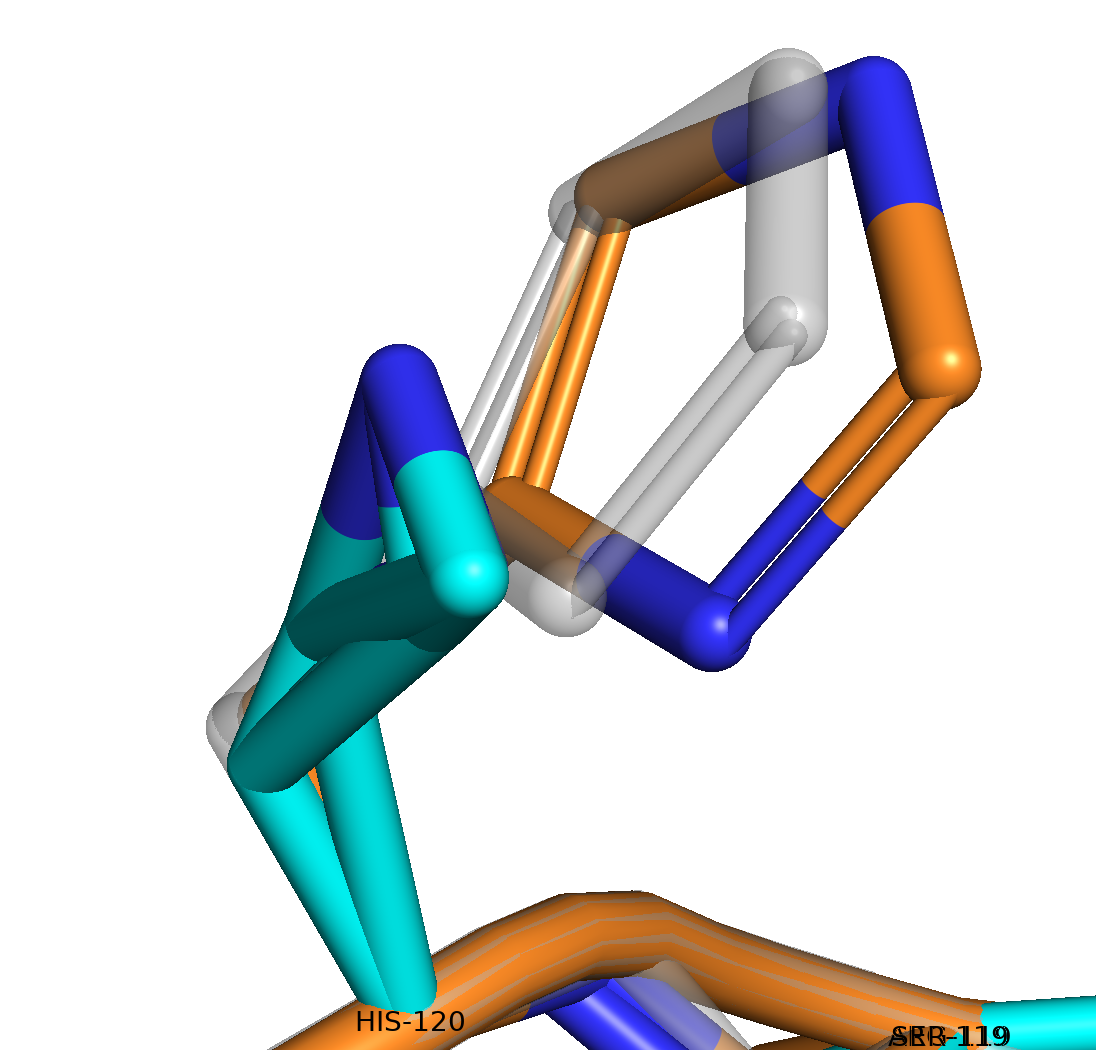
\includegraphics[width=\linewidth,height=55mm,keepaspectratio]{figures/results/failure-mode.png}
    \par\smallskip\textbf{(a)}
\end{minipage}\hfill
\begin{minipage}[t]{0.48\linewidth}
    \centering
    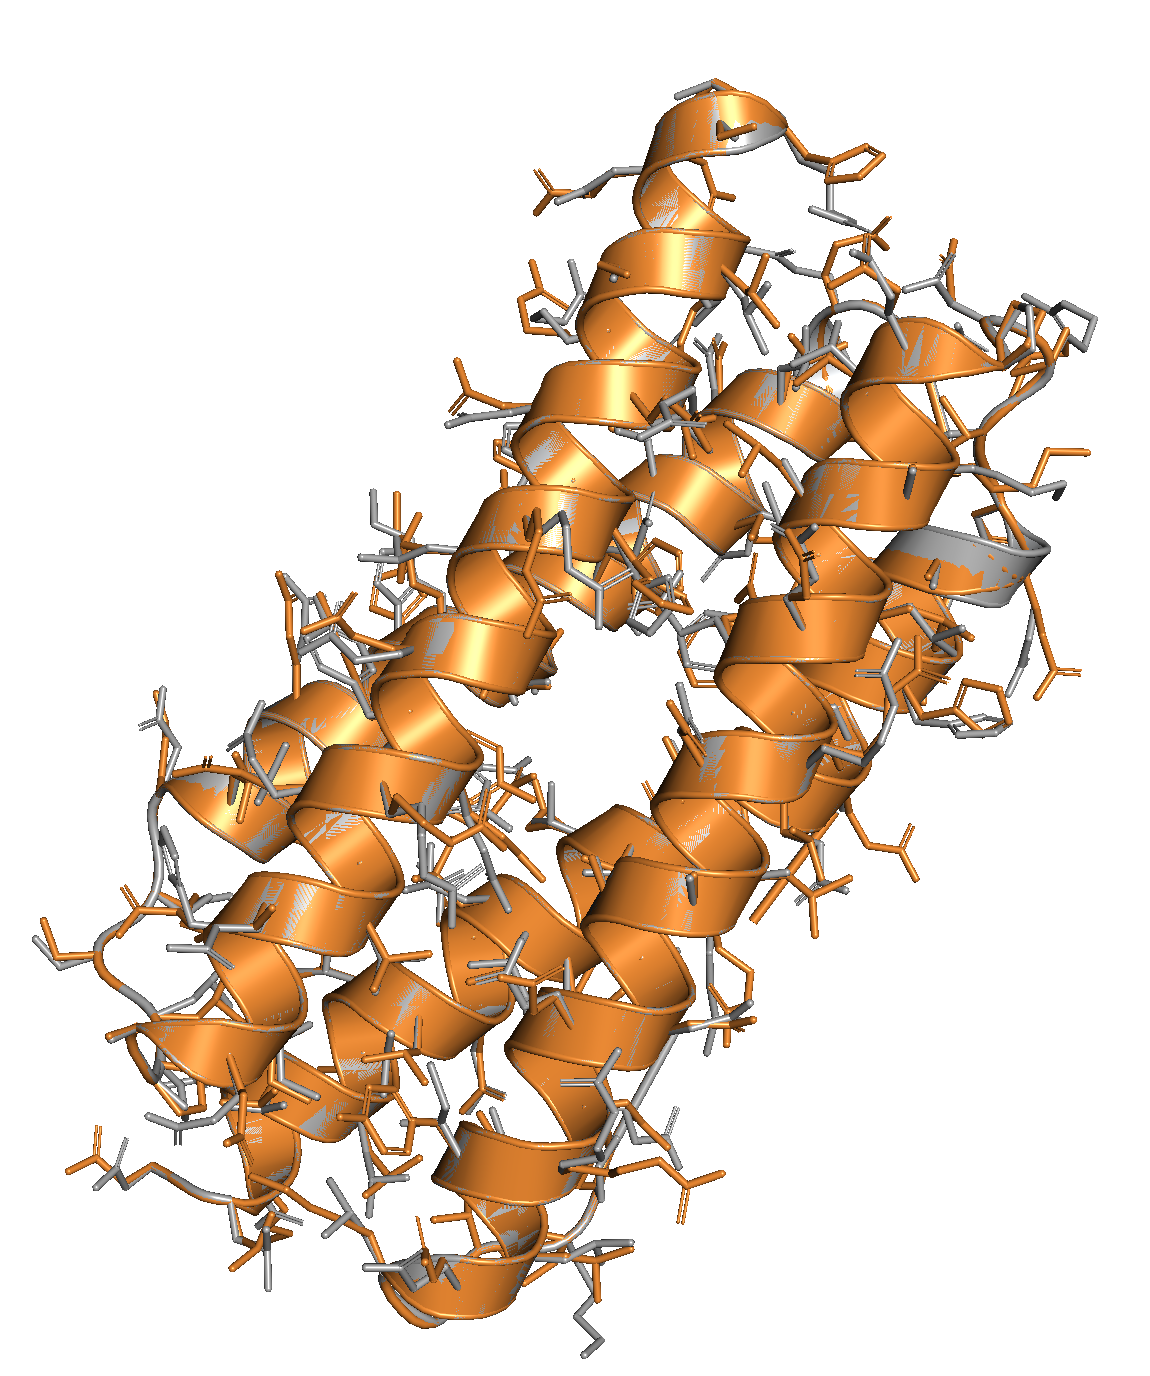
\includegraphics[width=\linewidth,height=55mm,keepaspectratio]{figures/results/reconst.png}
    \par\smallskip\textbf{(b)}
\end{minipage}
\caption{JEPA reconstruction examples. (a) HIS-120 in 5FLI chain A. The direct JEPA output (cyan) forms a chemically invalid local geometry, which is repaired by the postprocessing described in Section~\ref{sec:methods-reconstruction}. The native residue is transparent grey and the postprocessed reconstruction is orange. (b) Full-structure overlay for 4ETR chain A, with the native protein in grey and the postprocessed JEPA reconstruction in orange. Their backbones overlap closely, as expected from C$\alpha$ conditioning. Some side chains align well, while others retain angular or positional errors.}
\label{fig:reconstruction-postprocessed}
\end{figure}

\researchfindingbox{JEPA retains substantial sequence and structural information, but reconstructs atoms less accurately than the C$\alpha$ baseline.}

\subsection{Residue and Protein Organisation}
\label{sec:results-organisation}
\researchquestionbox{How do the latent spaces organise residue embeddings?}

\textbf{Linear probes.}
We evaluate amino-acid identity using two tests.
A linear classifier on the frozen embeddings predicts amino-acid identity with approximately 100\% accuracy for autoencoders, 69.3\% for random initialisation and 10.6\% for JEPA-70 (Table~\ref{tab:results-residue-probes}).
Amino-acid neighbour purity at $k=10$ is 100.0/99.9\% for the two autoencoders, 95.1\% for random initialisation, 45.1/45.3\% for absolute-position JEPA+SIGReg with 50/70\% masking and 21.7/23.0\% for JEPA with 50/70\% masking.
Thus, the autoencoders retain amino-acid identity almost perfectly, whereas uncropped LeJEPA shows the best secondary-structure (56.7\%). Relative-position JEPA+SIGReg with 50\% masking has the best RSA readout ($0.163$).
B-factor correlations are low across all models.

\par\bigskip\noindent
\begin{minipage}{\linewidth}
\centering
\setstretch{1}\fontsize{9.3}{11.1}\selectfont
\setlength{\tabcolsep}{4.3pt}
\begin{tabular}{lrrrr}
\toprule
Encoder & AA accuracy & SS accuracy & RSA $R^2$ & B-factor $\rho$ \\
\midrule
Random init. & 0.693 & 0.472 & 0.111 & 0.015 \\
$C_\alpha$ AE & 1.000 & 0.482 & 0.077 & 0.009 \\
Fully latent AE & 1.000 & 0.480 & 0.097 & 0.012 \\
JEPA 50 & 0.097 & 0.510 & 0.040 & 0.045 \\
JEPA 70 & 0.106 & 0.566 & 0.110 & 0.039 \\
JEPA mutation & 0.099 & 0.496 & 0.118 & 0.016 \\
JEPA+SIGReg 50 abs. & 0.097 & 0.476 & 0.007 & 0.069 \\
JEPA+SIGReg 70 abs. & 0.097 & 0.477 & 0.004 & 0.080 \\
JEPA+SIGReg mutation & 0.096 & 0.476 & 0.004 & 0.047 \\
JEPA+SIGReg 50 rel. & 0.097 & 0.482 & 0.163 & 0.036 \\
JEPA+SIGReg 70 rel. & 0.096 & 0.474 & 0.092 & 0.025 \\
LeJEPA, uncropped (EMA) & 0.099 & 0.567 & 0.029 & 0.014 \\
\bottomrule
\end{tabular}
\captionof{table}{Final-8D linear outputs for encoders at 100k and a random-init encoder, with probes for each case. AA = amino-acid identity. The uncropped LeJEPA row uses EMA weights.}
\label{tab:results-residue-probes}
\end{minipage}
\par\bigskip

Figure~\ref{fig:results-latent-organisation-100k} shows marked differences in latent-space organisation across selected models, with clearly separated amino-acid clusters in the autoencoder but more mixed identities in JEPA and LeJEPA.

\par\addvspace{1.5\baselineskip}\noindent
\begin{minipage}{\linewidth}
\centering
\makebox[\linewidth][c]{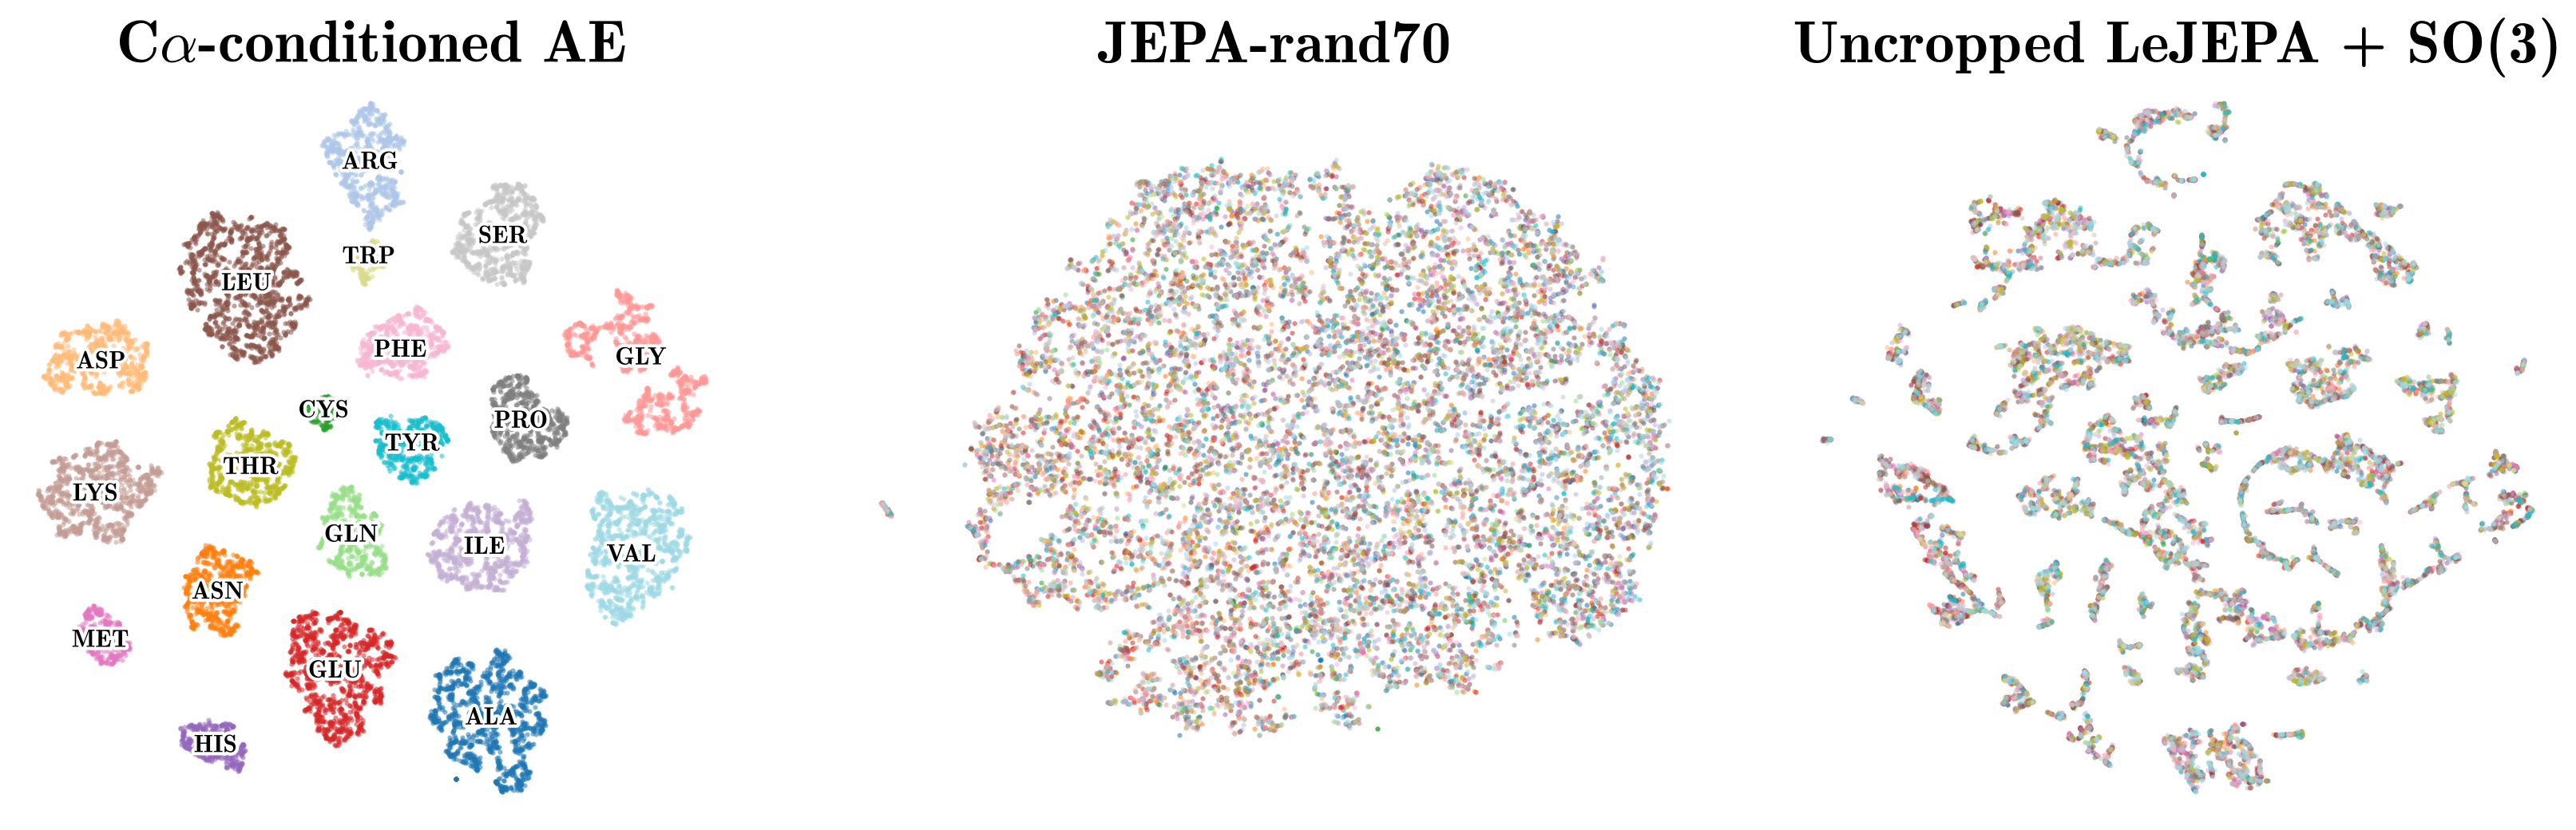
\includegraphics[width=1.04\linewidth]{figures/results/tsne_aa_ca_cond_jepa70_uncropped_lejepa_so3_100k.png}}
\captionof{figure}{t-SNE projections of residue embeddings from the C$\alpha$-conditioned autoencoder (left), JEPA with 70\% random masking (middle), and uncropped LeJEPA + SO(3) (right), at 100k checkpoints. Different colours represent different amino acids, labelled in the AE subfigure.}
\label{fig:results-latent-organisation-100k}
\end{minipage}
\par\addvspace{1.5\baselineskip}

\textbf{Absolute residue index.}
The downstream performance difference between absolute- and relative-position JEPA+SIGReg raises the question of how positional information influences the learned representations.
We use t-SNE to visualise which residues form similar neighbourhoods in latent space and whether these neighbourhoods reflect properties such as residue identity or position.
Figure~\ref{fig:results-index-100k} compares JEPA+SIGReg with 50\% random masking using absolute (left) and relative positions (right), with residues coloured by their absolute index within the chain.
Repeated strands are visible in the absolute-position latent space, and its local neighbourhoods are ordered by residue index.
This reveals a shortcut in which absolute position becomes a dominant feature of the representation.
Using relative target-context offsets removes this strand structure.

Relative positioning reduces exact-index purity at $k=10$ from 94.27\% to 1.61\%. The fraction of queries whose closest neighbour shares the same index falls from 97.25\% to 6.43\%.
Thus, the absolute-position result mostly reflects residues at matching indices across different proteins.

\begin{figure}[htbp]
\vspace{0.4\baselineskip}
\centering
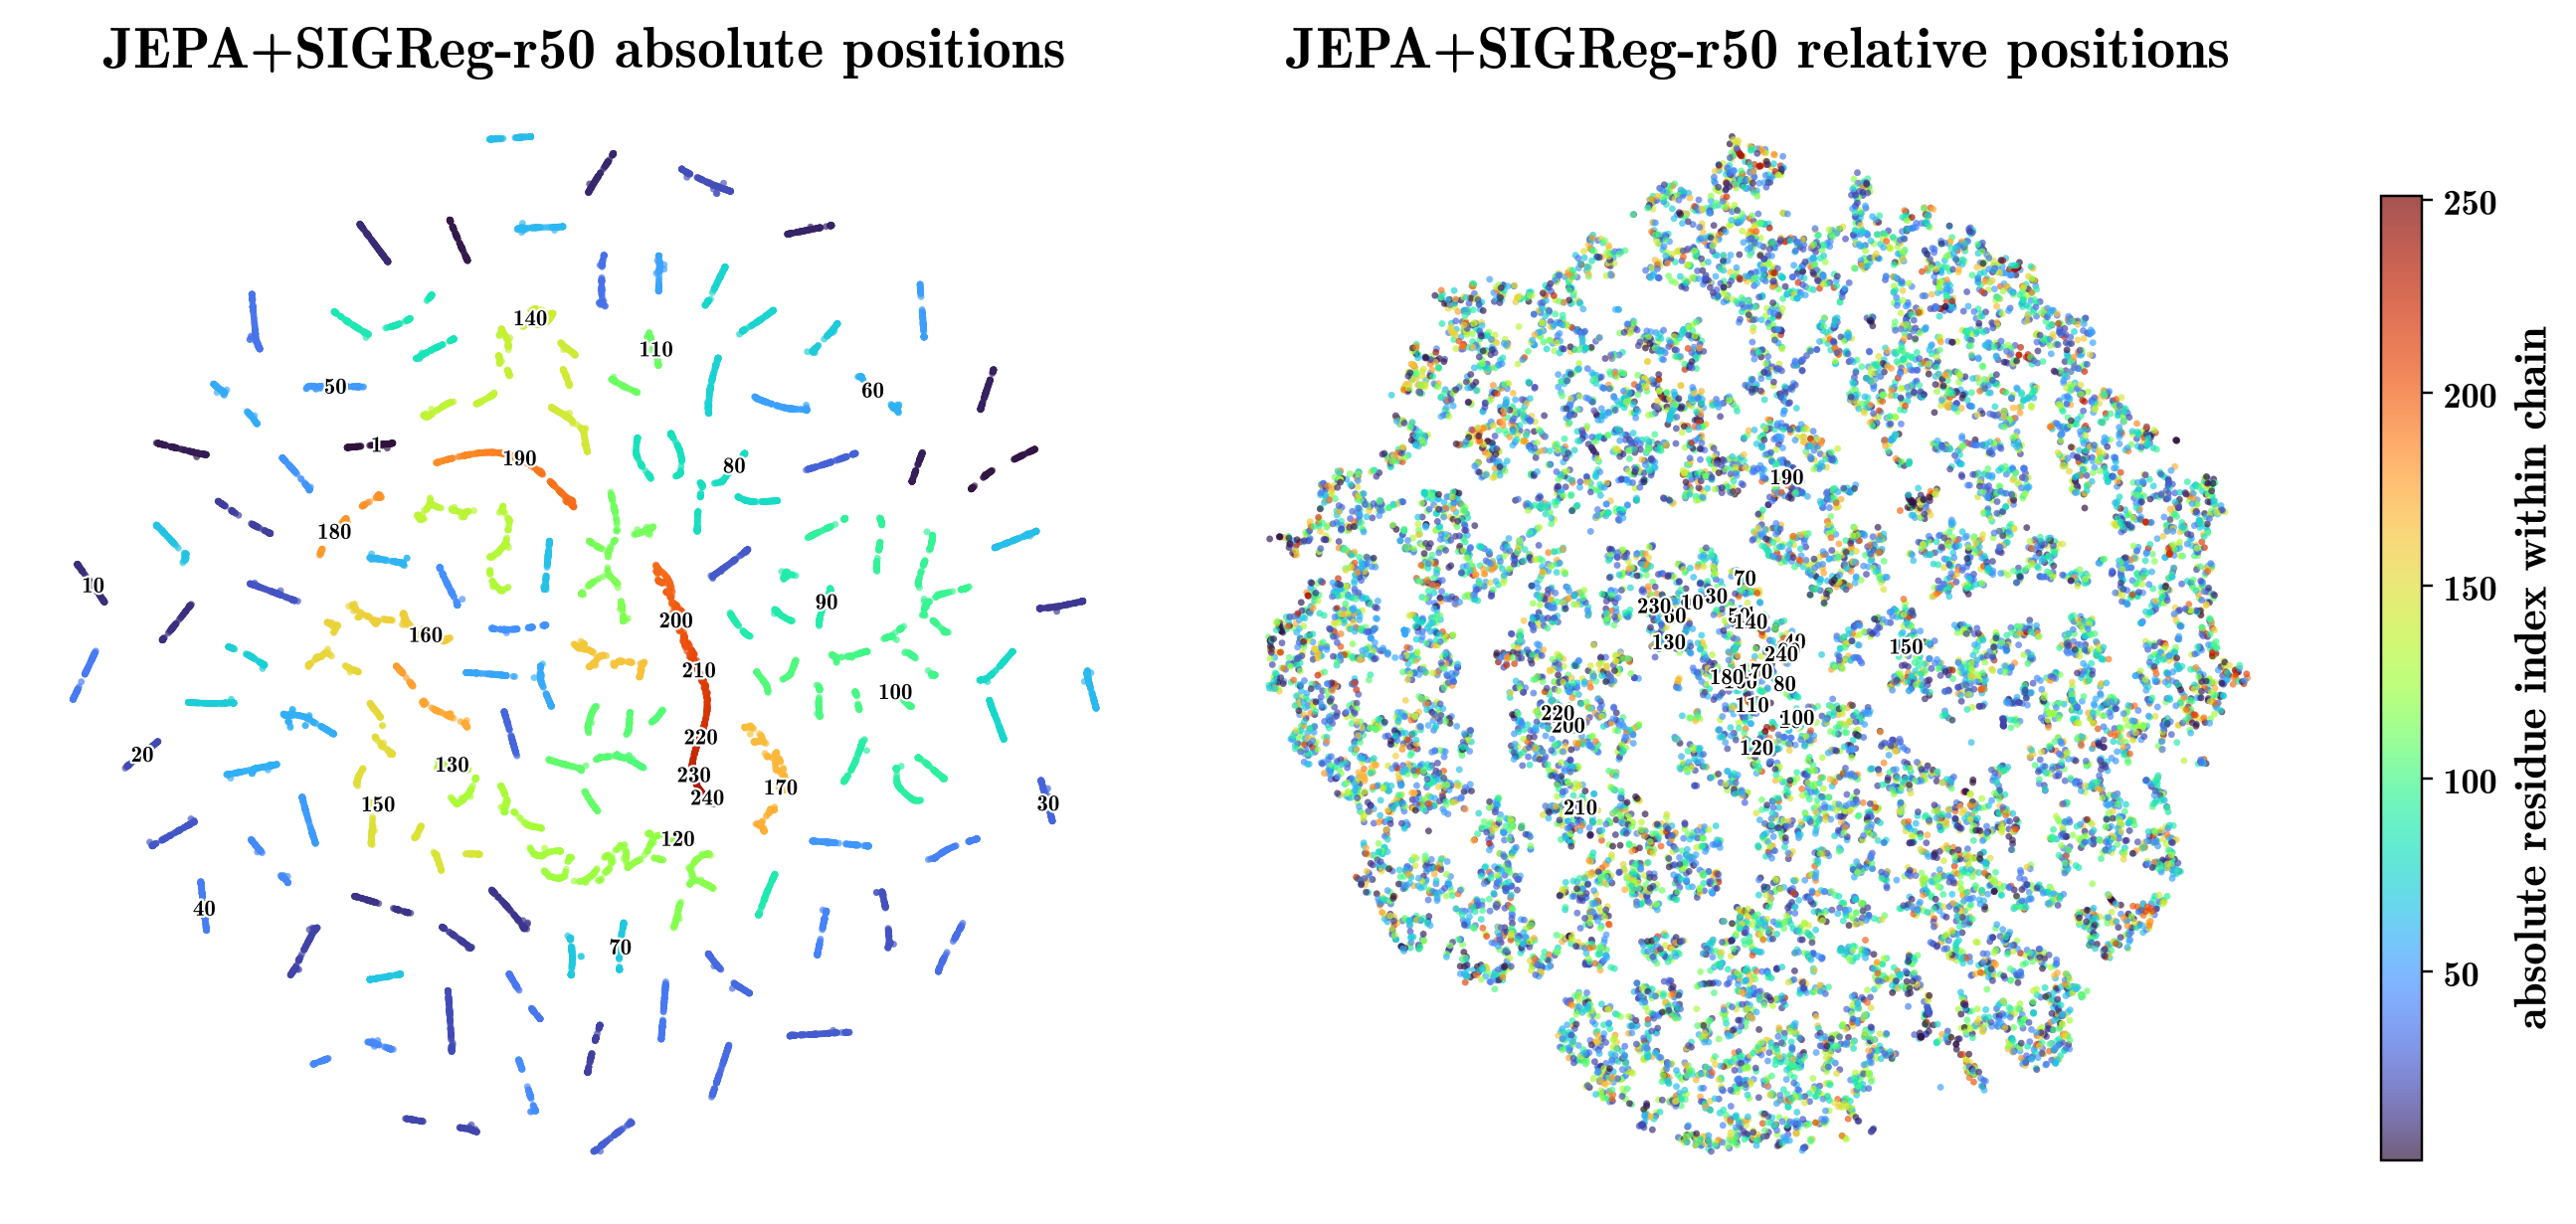
\includegraphics[width=\linewidth]{figures/results/tsne_lejepa-r50_absolute-v-relative_absolute-index_100k.png}
\caption{JEPA+SIGReg with 50\% random masking at 100k steps, using absolute positions (left) and relative positions (right). Numbers and colours on the strands indicate the absolute residue index within each chain, with an index range of [1-251].}
\label{fig:results-index-100k}
\vspace{0.4\baselineskip}
\end{figure}

Besides suppressing the residue-index shortcut, relative positioning also improves downstream performance.
For 70\% masking, it increases CatBio fold AUROC ($0.529$ to $0.733$) and FlexRMSF fold correlation ($0.108$ to $0.290$), and scores higher on 19/24 tasks. With 50\% masking, it improves on 18/24 tasks.
Although the relative-position model still receives pair features and signals from chain boundaries and length that can reveal approximate location, it removes the direct absolute target-position shortcut.


\textbf{Chain length.}
Uncropped LeJEPA also organises residues by chain length: residues from proteins of similar length form neighbourhoods in latent space (Figure~\ref{fig:results-chain-length-raw10k}).
In the cropped version, each crop has a fixed length, regardless of the protein's chain length.
To isolate the effect of cropping, we compare uncropped and cropped models while keeping every other setting unchanged, including 20\% global and 80\% local masking. Cropping reduces the chain-length correlation from $0.884$ to $0.193$, but effective rank also falls from $7.10$ to $1.61$. Retaining 80\% local masking means that only around ten visible residues remain in each 48-residue local crop, which appears too aggressive for the shorter view. We therefore use 50\% local masking in the reported cropped models, leaving around 24 visible residues and retaining near-full effective rank ($7.85/8$). The model also uses a larger batch, which, together with the lower masking rate, likely helps maintain this healthy rank.

\begin{figure}[htbp]
\vspace{0.4\baselineskip}
\centering
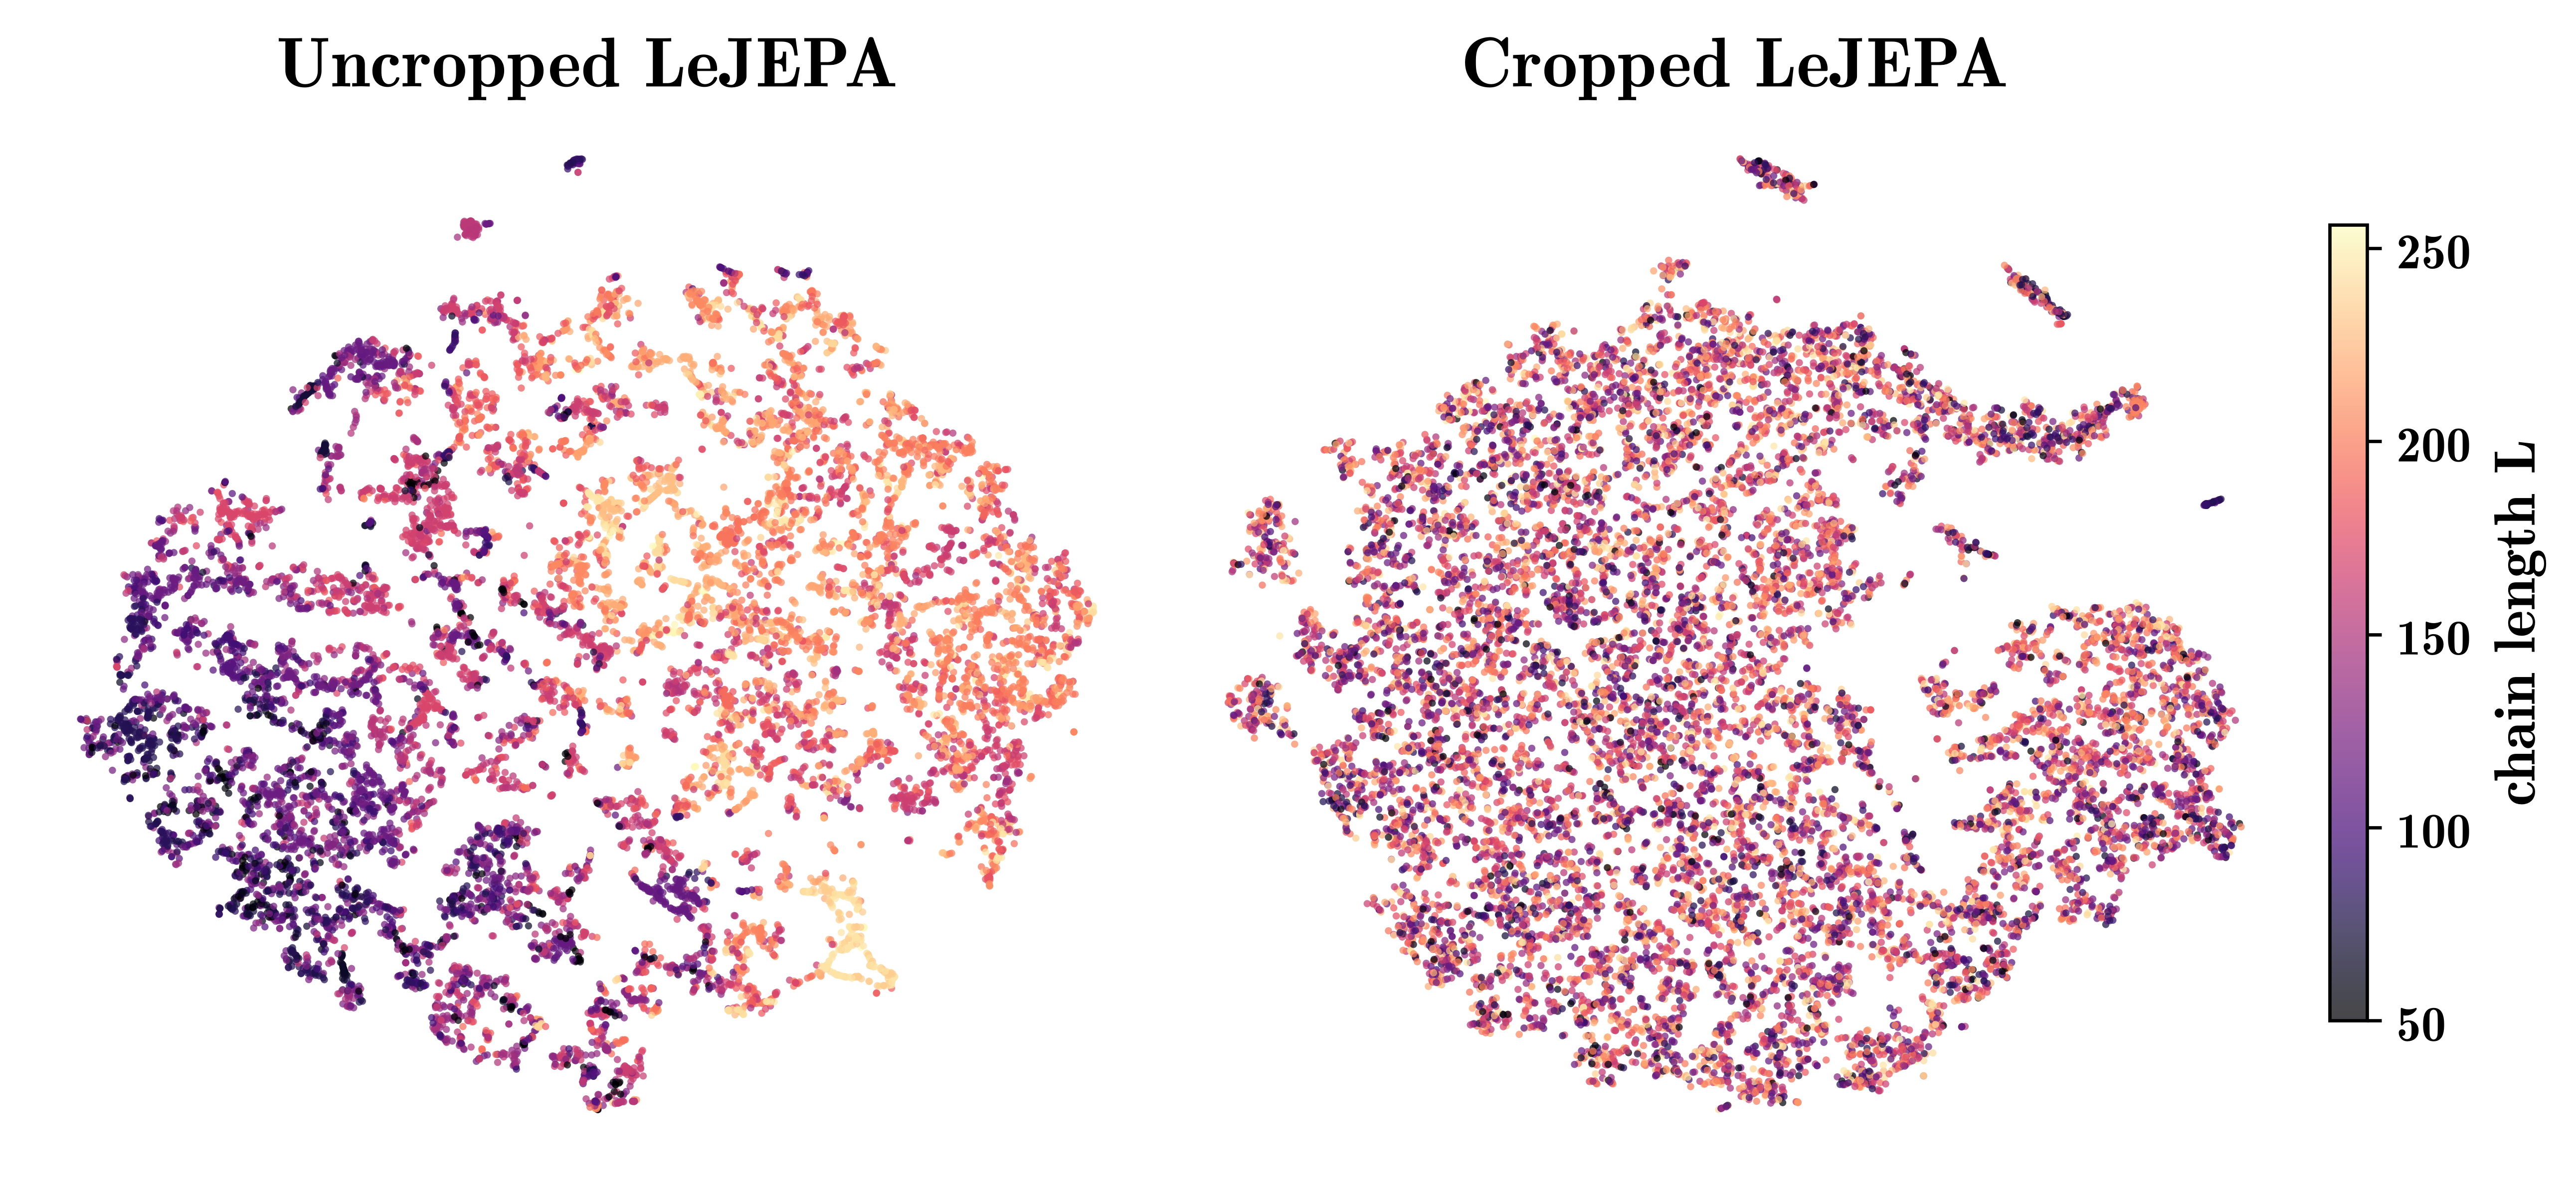
\includegraphics[width=0.95\linewidth]{figures/results/chain_length_tsne_matched_crop_control_raw10k.png}
\caption{Matched uncropped versus cropped LeJEPA comparison at the raw 10k checkpoint. Both models use mean-pooled protein views and differ only in cropping. Residue embeddings are coloured by chain length. Chain-length correlation decreases from $\rho=0.884$ to $0.193$, while effective rank decreases from $7.10$ to $1.61$.}
\label{fig:results-chain-length-raw10k}
\vspace{0.4\baselineskip}
\end{figure}

\textbf{Protein-level structural neighbourhoods.}
Across the four representations, nearest latent neighbours have mean TM-score gains of $0.216$-$0.456$ over the length-matched controls. However, their mean sequence identity is also higher ($0.404$-$0.689$ versus $0.151$). Below 30\% sequence identity, mean TM-score differences range from $-0.028$ to $0.015$, with every 95\% confidence interval including zero. The selected latent spaces therefore group homologous, structurally related proteins, but do not show structural organisation beyond sequence similarity.


\textbf{Independent rotations.}
\label{sec:results-rotation-64d}
Figure~\ref{fig:results-rotation-64d-60k} compares 64D JEPA with 70\% random residue masking, without and with independently rotated context and target views at 60k.
The model trained with rotated views forms clearer amino-acid clusters.
A 10k checkpoint rotation ablation in Appendix~\ref{app:latent-figures} shows that the same trend is present early on. However, a matched latent-width control shows that rotations alone are insufficient: with rotations in both models, the 64D representation forms amino-acid clusters whereas the 8D representation does not. Amino-acid neighbour purity falls from $0.974$ to $0.109$, suggesting that the 8D bottleneck discards much of the residue-identity information retained in 64D. Thus, the clustering reflects an interaction between rotation augmentation and latent capacity rather than rotations alone. These plots show changes in representation organisation, but do not establish rotation invariance.

\begin{figure}[htbp]
\centering
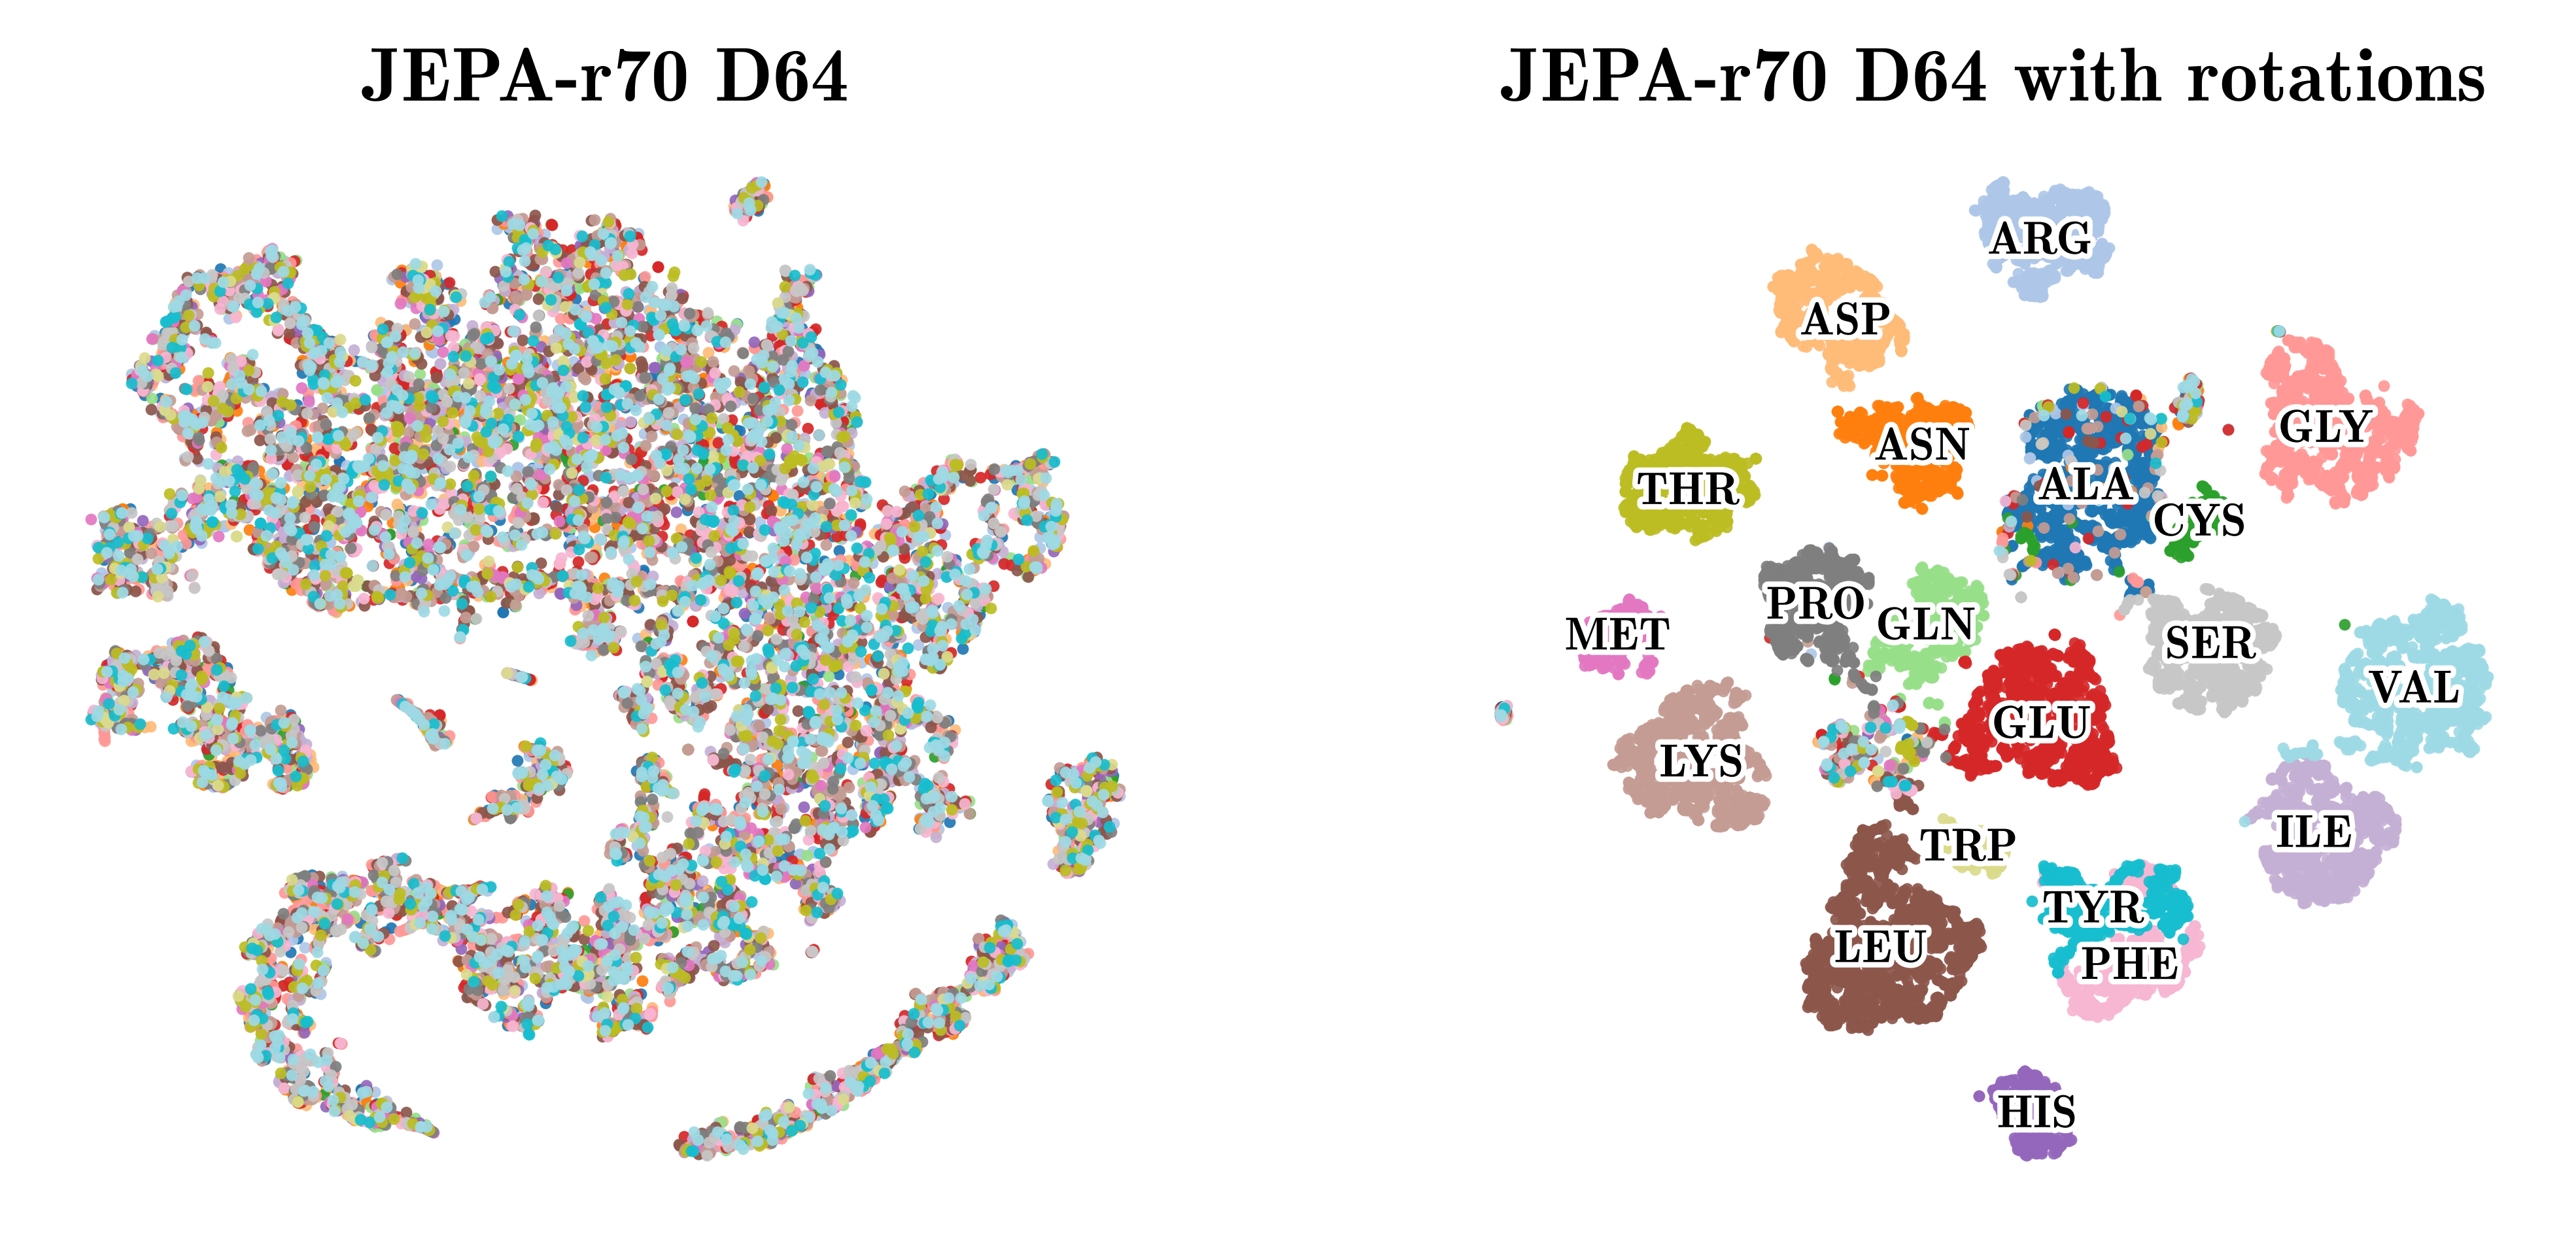
\includegraphics[width=0.88\linewidth]{figures/results/tsne_aa20_jepa-r70-d64-60k-v-rotation-60k_labels-on-clusters.png}
\caption{64D JEPA rotation comparison at 60k with 70\% random masking, without (left) and with (right) independent SO(3) view rotations. Different colours represent different amino acids, labelled in the rotated-view model.}
\label{fig:results-rotation-64d-60k}
\end{figure}
\researchfindingbox{Positional and geometric design choices strongly shape what information the learned representations retain. Relative positioning reduces absolute-index organisation and improves most downstream task scores, while independent rotation augmentation can produce clearer amino-acid clusters.}

\subsection{Rotation Invariance and Effective Rank}
\label{sec:results-collapse}

We monitor effective rank as a representation-health diagnostic and to detect collapse. For these 8D representations, a rank near one can indicate that most variation has collapsed into a single direction, whereas a higher rank can indicate healthier use of the latent space. However, higher rank does not necessarily guarantee better downstream performance.

Table~\ref{tab:results-rank-stb-10k} compares uncropped LeJEPA with and without independent SO(3) view rotations, retaining the same masking and objective settings. The rotated model has lower effective rank ($3.22$ versus $7.17$), yet scores higher on 21/24 tasks. The table shows four of these improvements. We suspected that this difference might be related to the effect of rotation augmentation rather than simple representation collapse. Our hypothesis was that learning from diverse rotated views removes orientation-dependent variation and concentrates the remaining information into fewer dimensions.

Therefore, we test rotation invariance. Across 400 chains (59,750 residues) and 16 rotations per chain, corresponding residue latents have mean protein-centred cosine similarity $0.765\;[0.756,0.774]$ with rotation training and $0.277\;[0.269,0.285]$ without it (95\% CIs). The increase occurs for every sampled protein, while randomly mismatched residues have similarities near zero. This supports our hypothesis and could explain the rotated model's lower effective rank. Further analysis is needed to determine what each latent dimension directly encodes.

\begin{table}[htbp]
\centering
\resultstableformat
\fontsize{9}{10.8}\selectfont
\setlength{\tabcolsep}{4pt}
\begin{tabular}{@{}lrrrrr@{}}
\toprule
Model & Rank /8 & \shortstack{BindShake\\AUROC} & \shortstack{CatBio fold\\AUROC} & \shortstack{FlexRMSF fold\\$\rho$} & \shortstack{Homo family\\macro-F1} \\
\midrule
Uncropped LeJEPA & 7.17 & 0.639 & 0.595 & 0.337 & 0.093 \\
Uncropped LeJEPA+SO(3) & 3.22 & \textbf{0.769} & \textbf{0.733} & \textbf{0.532} & \textbf{0.196} \\
\bottomrule
\end{tabular}
\caption{Uncropped LeJEPA at 10k (EMA weights) with and without rotations. SIGReg weight $0.02$ in both runs. Task scores use L600 STB evaluation.}
\label{tab:results-rank-stb-10k}
\end{table}

\subsection{Layerwise Information and the Latent Bottleneck}
\label{sec:results-layerwise}
\researchquestionbox{Is the final 8D latent the most useful representation for downstream tasks?}

Here, we examine encoder blocks 1, 6 and 12 and the final 8D latent mean of uncropped LeJEPA without rotations at 100k, starting from the model output and moving backwards through the encoder. Block 12 scores higher than the final 8D latent on 20/24 STB task scores, showing that more downstream-accessible information is available before the final projection.
Moving earlier in the encoder, block 6 scores higher than block 12 on 22/24 tasks and has the highest score among all four representations on 19/24. Both block outputs are 768-dimensional, so this comparison keeps the representation width fixed. Compared with the final 8D latent, BindShake AUROC increases from $0.585$ to $0.831$, FlexRMSF fold correlation from $0.225$ to $0.634$, and all six flexibility scores are higher.

Block 6 also exceeds the best final-8D score among the 18 models in main Table~\ref{tab:results-stb-main} on 22 of 24 task/split scores. The exceptions are Rep fold and Ept fold.
The largest gains are in flexibility: FlexRMSF fold ($0.634$ vs.\ $0.428$) and FlexNEQ fold ($0.514$ vs.\ $0.251$).
The progression is not monotonic: block 1 is strongest on BindBio fold and CatBio superfamily, block 12 on Con fold, and the final mean on Rep fold and Ept fold.
The random-init block-6 control is highest only on Rep fold, showing that the 768D input alone does not account for the improvements.

The same pattern appears in JEPA with 70\% random masking, where block 6 outperforms the final 8D latent on all nine evaluated task scores (Appendix~\ref{app:jepa-r70-layerwise}). Layerwise linear probes provide complementary evidence, with higher AA and SS accuracy in earlier blocks than in the final 8D latent (Appendix~\ref{app:layerwise-supporting}, Figure~\ref{fig:results-layer-probes}).

{\textbf{Encoder with six blocks.} Finally, we trained uncropped LeJEPA without rotations using six encoder blocks instead of twelve.
At 100k, its final 8D mean improves 15/24 scores over the 12-block model's final 8D mean, including all six flexibility scores (Appendix~\ref{app:encoder-depth}, Table~\ref{tab:results-encoder-depth}).
However, it remains below the original twelve-block encoder's intermediate block 6 on 23 of 24 scores. Thus, reducing encoder depth alone does not recover that performance.}

\researchfindingbox{Block 6 provides a more useful representation for most downstream tasks, exceeding the best final-8D score across all 18 main Table~\ref{tab:results-stb-main} entries on 22/24 task scores.}

\clearpage

\begin{table}[p]
\centering
\resultstableformat
\setlength{\tabcolsep}{1.8pt}
\renewcommand{\arraystretch}{0.86}
\caption{Full-L600 STB for uncropped LeJEPA without rotations at 100k, using raw weights and full-context evaluation. Scores are multiplied by 100. Higher is better, and row maxima are bold. The first four model columns are readouts from the 12-block encoder. Random-init block 6 is an untrained 768D control. The 768D and 8D readouts give the downstream head different input parameterisations. The final column gives the percentage change from the final 8D score to block 6. Large percentages arise when final-8D scores are near zero.}
\label{tab:results-layer-stb}
\sbox{\stbpreviewbox}{%
\begin{tabular}{@{}lllrrrrrr@{}}
\toprule
\multirow{2}{*}{Task type} & \multirow{2}{*}{Task} & \multirow{2}{*}{Split} & \multicolumn{4}{c}{12-block uncropped LeJEPA} & \multicolumn{1}{c}{Control} & \multicolumn{1}{c}{Change} \\[1.8pt]
& & & \shortstack{Block 1\\768D} & \shortstack{Block 6\\768D} & \shortstack{Block 12\\768D} & \shortstack{Final mean\\8D} & \shortstack{Random init.\\block 6, 768D} & \shortstack{$\Delta$ vs.\\final 8D (\%)} \\
\midrule
\multicolumn{9}{c}{\textbf{Functional-site prediction: AUROC $\times100$}} \\
\midrule
\multirow{5}{*}{Binding site}
& \multirow{2}{*}{BindInt} & Fold & 46.49 & \textbf{52.19} & 46.68 & 50.30 & 48.98 & +3.8 \\
& & SF & 93.16 & \textbf{94.13} & 90.96 & 88.45 & 88.06 & +6.4 \\
& \multirow{2}{*}{BindBio} & Fold & \textbf{78.35} & 78.31 & 71.32 & 59.32 & 74.12 & +32.0 \\
& & SF & 79.30 & \textbf{80.04} & 71.18 & 61.82 & 74.58 & +29.5 \\
& BindShake & Test & 79.61 & \textbf{83.11} & 80.38 & 58.45 & 78.23 & +42.2 \\
\multirow{4}{*}{Catalytic site}
& \multirow{2}{*}{CatInt} & Fold & 67.23 & \textbf{69.36} & 57.25 & 51.71 & 64.32 & +34.1 \\
& & SF & 94.48 & \textbf{95.78} & 88.98 & 80.74 & 88.95 & +18.6 \\
& \multirow{2}{*}{CatBio} & Fold & 83.27 & \textbf{85.05} & 80.17 & 53.67 & 81.87 & +58.5 \\
& & SF & \textbf{94.40} & 94.04 & 82.98 & 60.61 & 91.41 & +55.2 \\
\multirow{2}{*}{Conserved site}
& \multirow{2}{*}{Con} & Fold & 68.07 & 68.22 & \textbf{72.61} & 60.10 & 63.47 & +13.5 \\
& & SF & 88.83 & \textbf{92.16} & 84.21 & 77.27 & 81.40 & +19.3 \\
\multirow{2}{*}{Repeat motif}
& \multirow{2}{*}{Rep} & Fold & 67.95 & 60.39 & 53.50 & 71.05 & \textbf{76.66} & -15.0 \\
& & SF & 85.40 & \textbf{91.66} & 80.96 & 83.49 & 79.48 & +9.8 \\
\multirow{2}{*}{Epitope region}
& \multirow{2}{*}{Ept} & Fold & 55.58 & 55.70 & 61.36 & \textbf{62.00} & 55.61 & -10.2 \\
& & SF & 69.33 & \textbf{76.09} & 65.93 & 59.72 & 69.06 & +27.4 \\
\midrule
\multicolumn{9}{c}{\textbf{Remote homology: macro-F1 $\times100$}} \\
\midrule
\multirow{3}{*}{Remote homology}
& \multirow{3}{*}{Homo} & Fold & 14.56 & \textbf{16.94} & 9.68 & 6.73 & 6.64 & +151.7 \\
& & Family & 36.89 & \textbf{39.88} & 26.89 & 19.64 & 21.76 & +103.1 \\
& & SF & 17.19 & \textbf{19.90} & 8.52 & 5.54 & 6.77 & +259.2 \\
\midrule
\multicolumn{9}{c}{\textbf{Structural flexibility: Spearman's $\rho\times100$}} \\
\midrule
\multirow{6}{*}{Flexibility}
& \multirow{2}{*}{FlexRMSF} & Fold & 52.41 & \textbf{63.39} & 42.74 & 22.48 & 43.84 & +182.0 \\
& & SF & 53.13 & \textbf{68.52} & 52.51 & 30.96 & 41.73 & +121.3 \\
& \multirow{2}{*}{FlexBFactor} & Fold & 34.28 & \textbf{37.71} & 22.56 & 5.01 & 31.14 & +652.7 \\
& & SF & 29.65 & \textbf{32.73} & 20.58 & 3.50 & 27.15 & +835.1 \\
& \multirow{2}{*}{FlexNEQ} & Fold & 46.97 & \textbf{51.39} & 39.73 & 2.46 & 19.11 & +1989.0 \\
& & SF & 46.70 & \textbf{50.69} & 39.76 & 3.54 & 19.29 & +1331.9 \\
\bottomrule
\end{tabular}%
}
\stbpreviewfit
\end{table}
\clearpage

\subsection{Discussion}
\label{sec:results-discussion}

This discussion connects the downstream, latent-space, reconstruction and layerwise results, interpreting what the models retain and where the objectives introduce trade-offs or shortcuts. We examine how the objective and design choices shape which information remains accessible.

\subsubsection{Predictive Objectives and Downstream Transfer}

The central question of this thesis is whether predicting or aligning latent representations can capture information useful for protein structure and function. The results support this idea, but no model is uniformly strongest. Because StructTokenBench spans residue- and protein-level properties, the task-specific results show that information useful at one biological scale is not automatically strongest at another. Together with the differences in latent-space organisation, this suggests that the objective and view construction shape which information remains accessible rather than making a representation uniformly better or worse.
Mutation conditioning extends this question to interventions (Section~\ref{sec:results-mutation}). Its downstream changes remain difficult to isolate because the action input, mutant target and training loss change together. It should therefore be interpreted as a first implementation of mutation actions rather than a complete mutation model.

\subsubsection{Masking and Shortcut Learning}

The benefit of 70\% random masking in JEPA is consistent with I-JEPA's finding that sufficiently informative targets are important for latent prediction \citep{assran2023ijepa}. Masking changes both task difficulty and the shortcuts available to solve it, so harder prediction helps only when the model must use meaningful context. With learned absolute target positions, JEPA+SIGReg can organise its latent space almost directly by residue index. Relative offsets retain sequence separation while removing this direct identifier, and the simultaneous reduction in index purity and improvement in downstream scores indicates that the shortcut had displaced more useful information. In LeJEPA, complete protein views expose the same chain length across views, whereas fixed-length crops reduce that organisation. The matched crop experiment also shows why only removing shortcuts is not enough. Chain-length correlation falls, but effective rank also falls to $1.61/8$, indicating that most variation is concentrated in very few directions (Section~\ref{sec:results-organisation}). A protein-specific view must therefore remove easy global or local shortcuts without making the remaining prediction problem uninformative or excessively difficult.

\subsubsection{Invariance and Representation Collapse}

Because protein properties should not depend on global orientation, we expected independent rotations to improve the learned representations more broadly. Rotations make corresponding residue embeddings substantially more consistent under changes in global orientation, but their downstream effect remains task- and model-dependent (Section~\ref{sec:results-collapse}). Similarly, SIGReg is necessary to prevent near-constant branches in JEPA+SIGReg, yet a near-full effective rank does not guarantee useful transfer. Rotated LeJEPA shows that the opposite can also occur, as fewer dominant directions coexist with stronger performance on most evaluated tasks. Thus, invariance and effective rank describe properties of a representation rather than its overall quality. Effective rank is best interpreted as a warning signal for dimensional collapse, alongside downstream and property-specific evaluations, rather than an objective we should maximise.

\subsubsection{Reconstruction Quality}

The reconstruction gap is expected because JEPA predicts latent representations and training never optimises the encoder for atom-level reconstruction. Reconstruction therefore tests how much atomic detail remains accessible, rather than whether JEPA can match an autoencoder trained for this task. The C$\alpha$ TM-score is 1.0 for all outputs because those coordinates are provided directly, so it cannot establish that JEPA recovers the global fold. The common-atom lDDT is higher than the true-sequence lDDT because sequence errors exclude some poorly reconstructed side-chain atoms from the common-atom metric. One possible explanation for the chemically invalid decoder geometries is that the coordinate and sequence losses do not explicitly enforce valid bond lengths, bond angles or separation between atoms. When several side-chain placements are possible, coordinate optimisation can also favour an average that is not a valid geometry. Postprocessing makes the structures more realistic, but its worse side-chain reconstruction metrics show that it can move atoms away from their native positions. Postprocessing is therefore useful for visualisation, without necessarily improving reconstruction.

\subsubsection{Intermediate Encoder Representations}

The block 12 result suggests that the final projection may discard downstream-accessible information, but it cannot separate the effect of the projection from the reduction to eight dimensions. The block 6 comparison is more direct because blocks 6 and 12 have the same width. Its stronger scores suggest that useful downstream features peak earlier in the encoder and may later become specialised or compressed. This does not mean that six encoder blocks are sufficient, since training a separate six-block model does not reproduce the intermediate output. Previous work similarly finds that intermediate representations can outperform final layers and explains this through the balance between preserving information and compressing it for the training objective \citep{skean2025layer}. Other protein language model studies also find that the best layer depends on the downstream task, and that many tasks reuse features learned before the final layer \citep{li2024featurereuse,joeres2026taskdataset}. Even with the dimensionality confound, these results highlight the importance of choosing which encoder layer to evaluate and place our structural encoder within the same broader pattern of useful intermediate representations (Section~\ref{sec:results-layerwise}).

\clearpage

\clearpage
\endinput
%TC:ignore
\appendix
\section{Downstream Results for Proteins up to 256 Residues}
\label{app:l256}
Table~\ref{tab:results-stb-l256} reports StructTokenBench results for proteins with at most 256 residues.
\begingroup
\ifdefined\stbworkshopbox\else\newsavebox{\stbworkshopbox}\fi
\providecommand{\stbworkshopfit}{\ifdim\wd\stbworkshopbox>\linewidth\resizebox{\linewidth}{!}{\usebox{\stbworkshopbox}}\else\usebox{\stbworkshopbox}\fi}
\begin{table}[p]
\centering
\resultstableformat
\setlength{\tabcolsep}{2pt}
\renewcommand{\arraystretch}{0.88}
\fontsize{7.5}{9}\selectfont
\caption{StructTokenBench evaluation restricted to proteins with at most 256 residues.}
\label{tab:results-stb-l256}
\sbox{\stbworkshopbox}{%
\begin{tabular}{@{}lllrrrrrrrr@{}}
\toprule
\multirow{2}{*}{Task type} & \multirow{2}{*}{Task} & \multirow{2}{*}{Split} & \multicolumn{2}{c}{Autoencoders} & \multicolumn{3}{c}{JEPA} & \multicolumn{3}{c}{JEPA+SIGReg} \\[1.8pt]
 & & & $C_\alpha$ & Full AE & 50\% & 70\% & Mut. & 50\% & 70\% & Mut. \\
\midrule
\multicolumn{11}{c}{\textbf{Functional-site prediction: AUROC $\times100$}} \\
\midrule
\multirow{5}{*}{Binding site} & \multirow{2}{*}{BindInt} & Fold & 41.69 & 40.66 & 40.54 & 42.03 & \textbf{42.14} & 38.91 & 40.65 & 39.69 \\
 &  & SF & 86.84 & 85.80 & 87.39 & 86.07 & 86.82 & \textbf{89.52} & 83.70 & 88.85 \\
 & \multirow{2}{*}{BindBio} & Fold & 62.96 & \textbf{65.32} & 55.60 & 58.54 & 57.47 & 57.12 & 57.47 & 57.16 \\
 &  & SF & 63.23 & \textbf{65.63} & 58.22 & 60.02 & 59.49 & 59.60 & 59.79 & 59.73 \\
 & BindShake & Test & 59.19 & \textbf{65.11} & 53.76 & 64.42 & 63.89 & 59.73 & 59.96 & 60.83 \\
\multirow{4}{*}{Catalytic site} & \multirow{2}{*}{CatInt} & Fold & 58.97 & \textbf{61.19} & 58.92 & 58.09 & 59.94 & 59.38 & 58.19 & 57.39 \\
 &  & SF & 76.50 & \textbf{76.82} & 73.79 & 75.37 & 75.36 & 74.33 & 75.91 & 76.47 \\
 & \multirow{2}{*}{CatBio} & Fold & 64.01 & \textbf{71.89} & 54.46 & 62.41 & 60.40 & 53.05 & 51.54 & 51.53 \\
 &  & SF & 78.31 & \textbf{84.44} & 65.48 & 71.96 & 69.87 & 62.06 & 61.68 & 63.21 \\
\multirow{2}{*}{Conserved site} & \multirow{2}{*}{Con} & Fold & 57.20 & \textbf{59.98} & 59.51 & 58.51 & 59.34 & 58.85 & 59.43 & 59.22 \\
 &  & SF & 71.97 & 73.48 & 70.73 & 71.22 & 72.43 & \textbf{74.30} & 74.10 & 74.11 \\
\multirow{2}{*}{Repeat motif} & \multirow{2}{*}{Rep} & Fold & 65.38 & 64.43 & 66.08 & 65.91 & 65.37 & \textbf{67.73} & 66.97 & 67.08 \\
 &  & SF & 80.79 & 79.82 & \textbf{82.00} & 79.24 & 81.25 & 77.65 & 76.02 & 77.46 \\
\multirow{2}{*}{Epitope region} & \multirow{2}{*}{Ept} & Fold & 56.28 & 55.21 & \textbf{59.29} & 54.79 & 56.57 & 58.34 & 56.67 & 55.90 \\
 &  & SF & 64.15 & 62.59 & \textbf{65.09} & 60.61 & 61.86 & 61.02 & 60.76 & 57.63 \\
\midrule
\multicolumn{11}{c}{\textbf{Remote homology: macro-F1 $\times100$}} \\
\midrule
\multirow{3}{*}{Remote homology} & \multirow{3}{*}{Homo} & Fold & 7.89 & 6.29 & 7.10 & \textbf{10.21} & 8.77 & 7.43 & 7.98 & 8.54 \\
 &  & Family & \textbf{35.26} & 26.86 & 17.67 & 21.29 & 17.00 & 21.52 & 20.01 & 26.60 \\
 &  & SF & 8.41 & 10.47 & 4.97 & \textbf{11.59} & 8.51 & 7.73 & 6.67 & 6.14 \\
\midrule
\multicolumn{11}{c}{\textbf{Structural flexibility: Spearman's $\rho\times100$}} \\
\midrule
\multirow{6}{*}{Flexibility} & \multirow{2}{*}{FlexRMSF} & Fold & 14.98 & \textbf{45.34} & 26.50 & 30.46 & 30.76 & 12.12 & 10.48 & 10.31 \\
 &  & SF & 13.96 & \textbf{44.34} & 31.68 & 28.47 & 33.10 & 10.26 & 10.24 & 8.45 \\
 & \multirow{2}{*}{FlexBFactor} & Fold & 11.21 & \textbf{26.00} & 1.80 & 19.62 & 16.25 & 1.91 & 3.32 & 2.80 \\
 &  & SF & 11.26 & \textbf{26.94} & 12.97 & 22.10 & 23.40 & 4.01 & 3.56 & 4.92 \\
 & \multirow{2}{*}{FlexNEQ} & Fold & 15.98 & 24.95 & 10.52 & \textbf{33.38} & 16.92 & 7.98 & 7.75 & 7.80 \\
 &  & SF & 13.51 & 22.11 & 11.43 & \textbf{29.19} & 10.87 & 6.61 & 6.82 & 6.63 \\
\bottomrule
\end{tabular}%
}
\stbworkshopfit
\end{table}

\clearpage
\endgroup
\section{Early Latent-space Rotation Comparison}
\label{app:latent-figures}
Figure~\ref{fig:results-rotation-64d-10k} compares 64D JEPA with 70\% random residue masking, without and with independently rotated context and target views at 10k.

\begin{figure}[htbp]
\centering
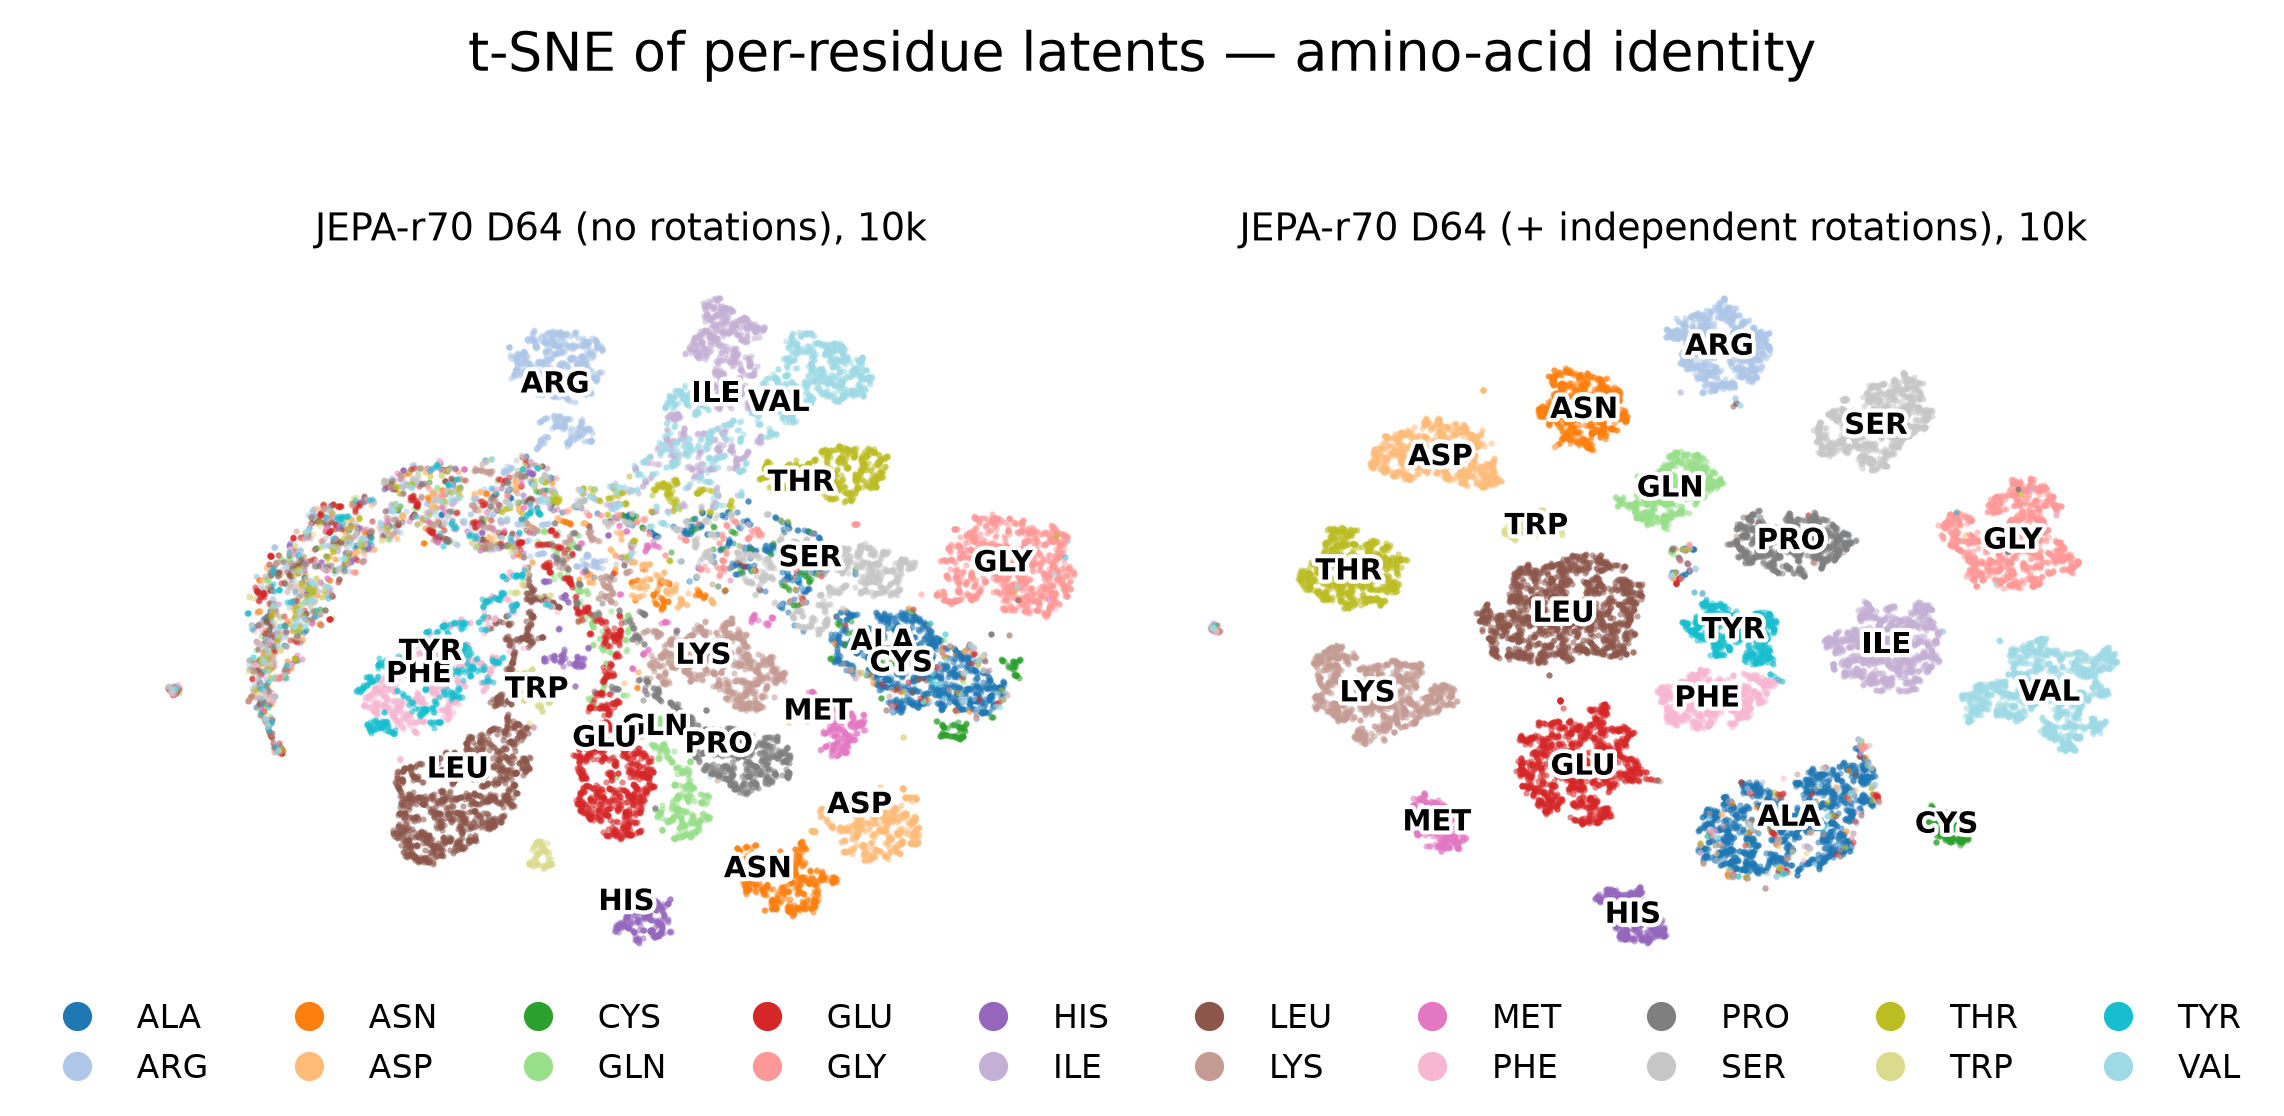
\includegraphics[width=0.88\linewidth]{figures/results/tsne_aa20_jepa-r70-d64-no-rotation-v-rotation_labels-on-clusters.png}
\caption{Matched 10k 64D JEPA rotation diagnostic, with 70\% random masking and points coloured by amino-acid identity. The existing workshop plot uses the same 15,000 sampled residues and visualisation settings in both panels. Cluster separation is qualitative t-SNE evidence, not a quantitative test of rotation invariance or downstream transfer.}
\label{fig:results-rotation-64d-10k}
\end{figure}
\clearpage
\section{Supporting Layerwise Evaluation}
\label{app:layerwise-supporting}
\label{app:jepa-r70-layerwise}
The matched JEPA random-70 evaluation is complete at all three hidden blocks for BindInt, BindBio, BindShake, CatInt and CatBio.
Across these nine task/split scores, block 6 exceeds the final 8D latent in both model families; it is the strongest of the four readouts on 7/9 canonical LeJEPA scores and 5/9 JEPA scores (Tables~\ref{tab:results-layer-stb} and~\ref{tab:results-layer-stb-jepa-r70}).
This recurrence indicates that the middle-layer advantage is not unique to the canonical LeJEPA objective, although the JEPA comparison currently covers only this five-task subset.

\begin{table}[p]
\centering
\resultstableformat
\setlength{\tabcolsep}{2pt}
\renewcommand{\arraystretch}{0.92}
\caption{Completed layerwise STB for JEPA with 70\% random masking, using raw/online weights at 100k and full-context evaluation. Hidden-block outputs are 768D and the final latent mean is 8D. Scores are multiplied by 100; bold marks the strongest readout for each task/split.}
\label{tab:results-layer-stb-jepa-r70}
\begin{tabular}{@{}llrrrr@{}}
\toprule
\multirow{2}{*}{Task} & \multirow{2}{*}{Split}
& \multicolumn{4}{c}{JEPA, random 70\%} \\[1.8pt]
& & Block 1 & Block 6 & Block 12 & Final 8D \\
\midrule
\multirow{2}{*}{BindInt}
& Fold & 47.86 & \textbf{48.86} & 48.24 & 47.11 \\
& SF   & 88.24 & \textbf{91.95} & 91.59 & 80.06 \\
\multirow{2}{*}{BindBio}
& Fold & 72.61 & \textbf{73.22} & 72.84 & 65.56 \\
& SF   & 72.93 & \textbf{73.85} & 73.76 & 65.31 \\
BindShake
& Test & 78.23 & 78.13 & \textbf{78.38} & 71.85 \\
\multirow{2}{*}{CatInt}
& Fold & 65.69 & \textbf{65.72} & 65.05 & 56.84 \\
& SF   & 88.00 & 91.79 & \textbf{92.00} & 76.71 \\
\multirow{2}{*}{CatBio}
& Fold & \textbf{80.72} & 80.13 & 78.23 & 71.50 \\
& SF   & 89.81 & 89.62 & \textbf{90.39} & 75.36 \\
\bottomrule
\end{tabular}
\end{table}
\clearpage

\paragraph{LeJEPA linear probes.}
\begin{figure}[htbp]
\centering
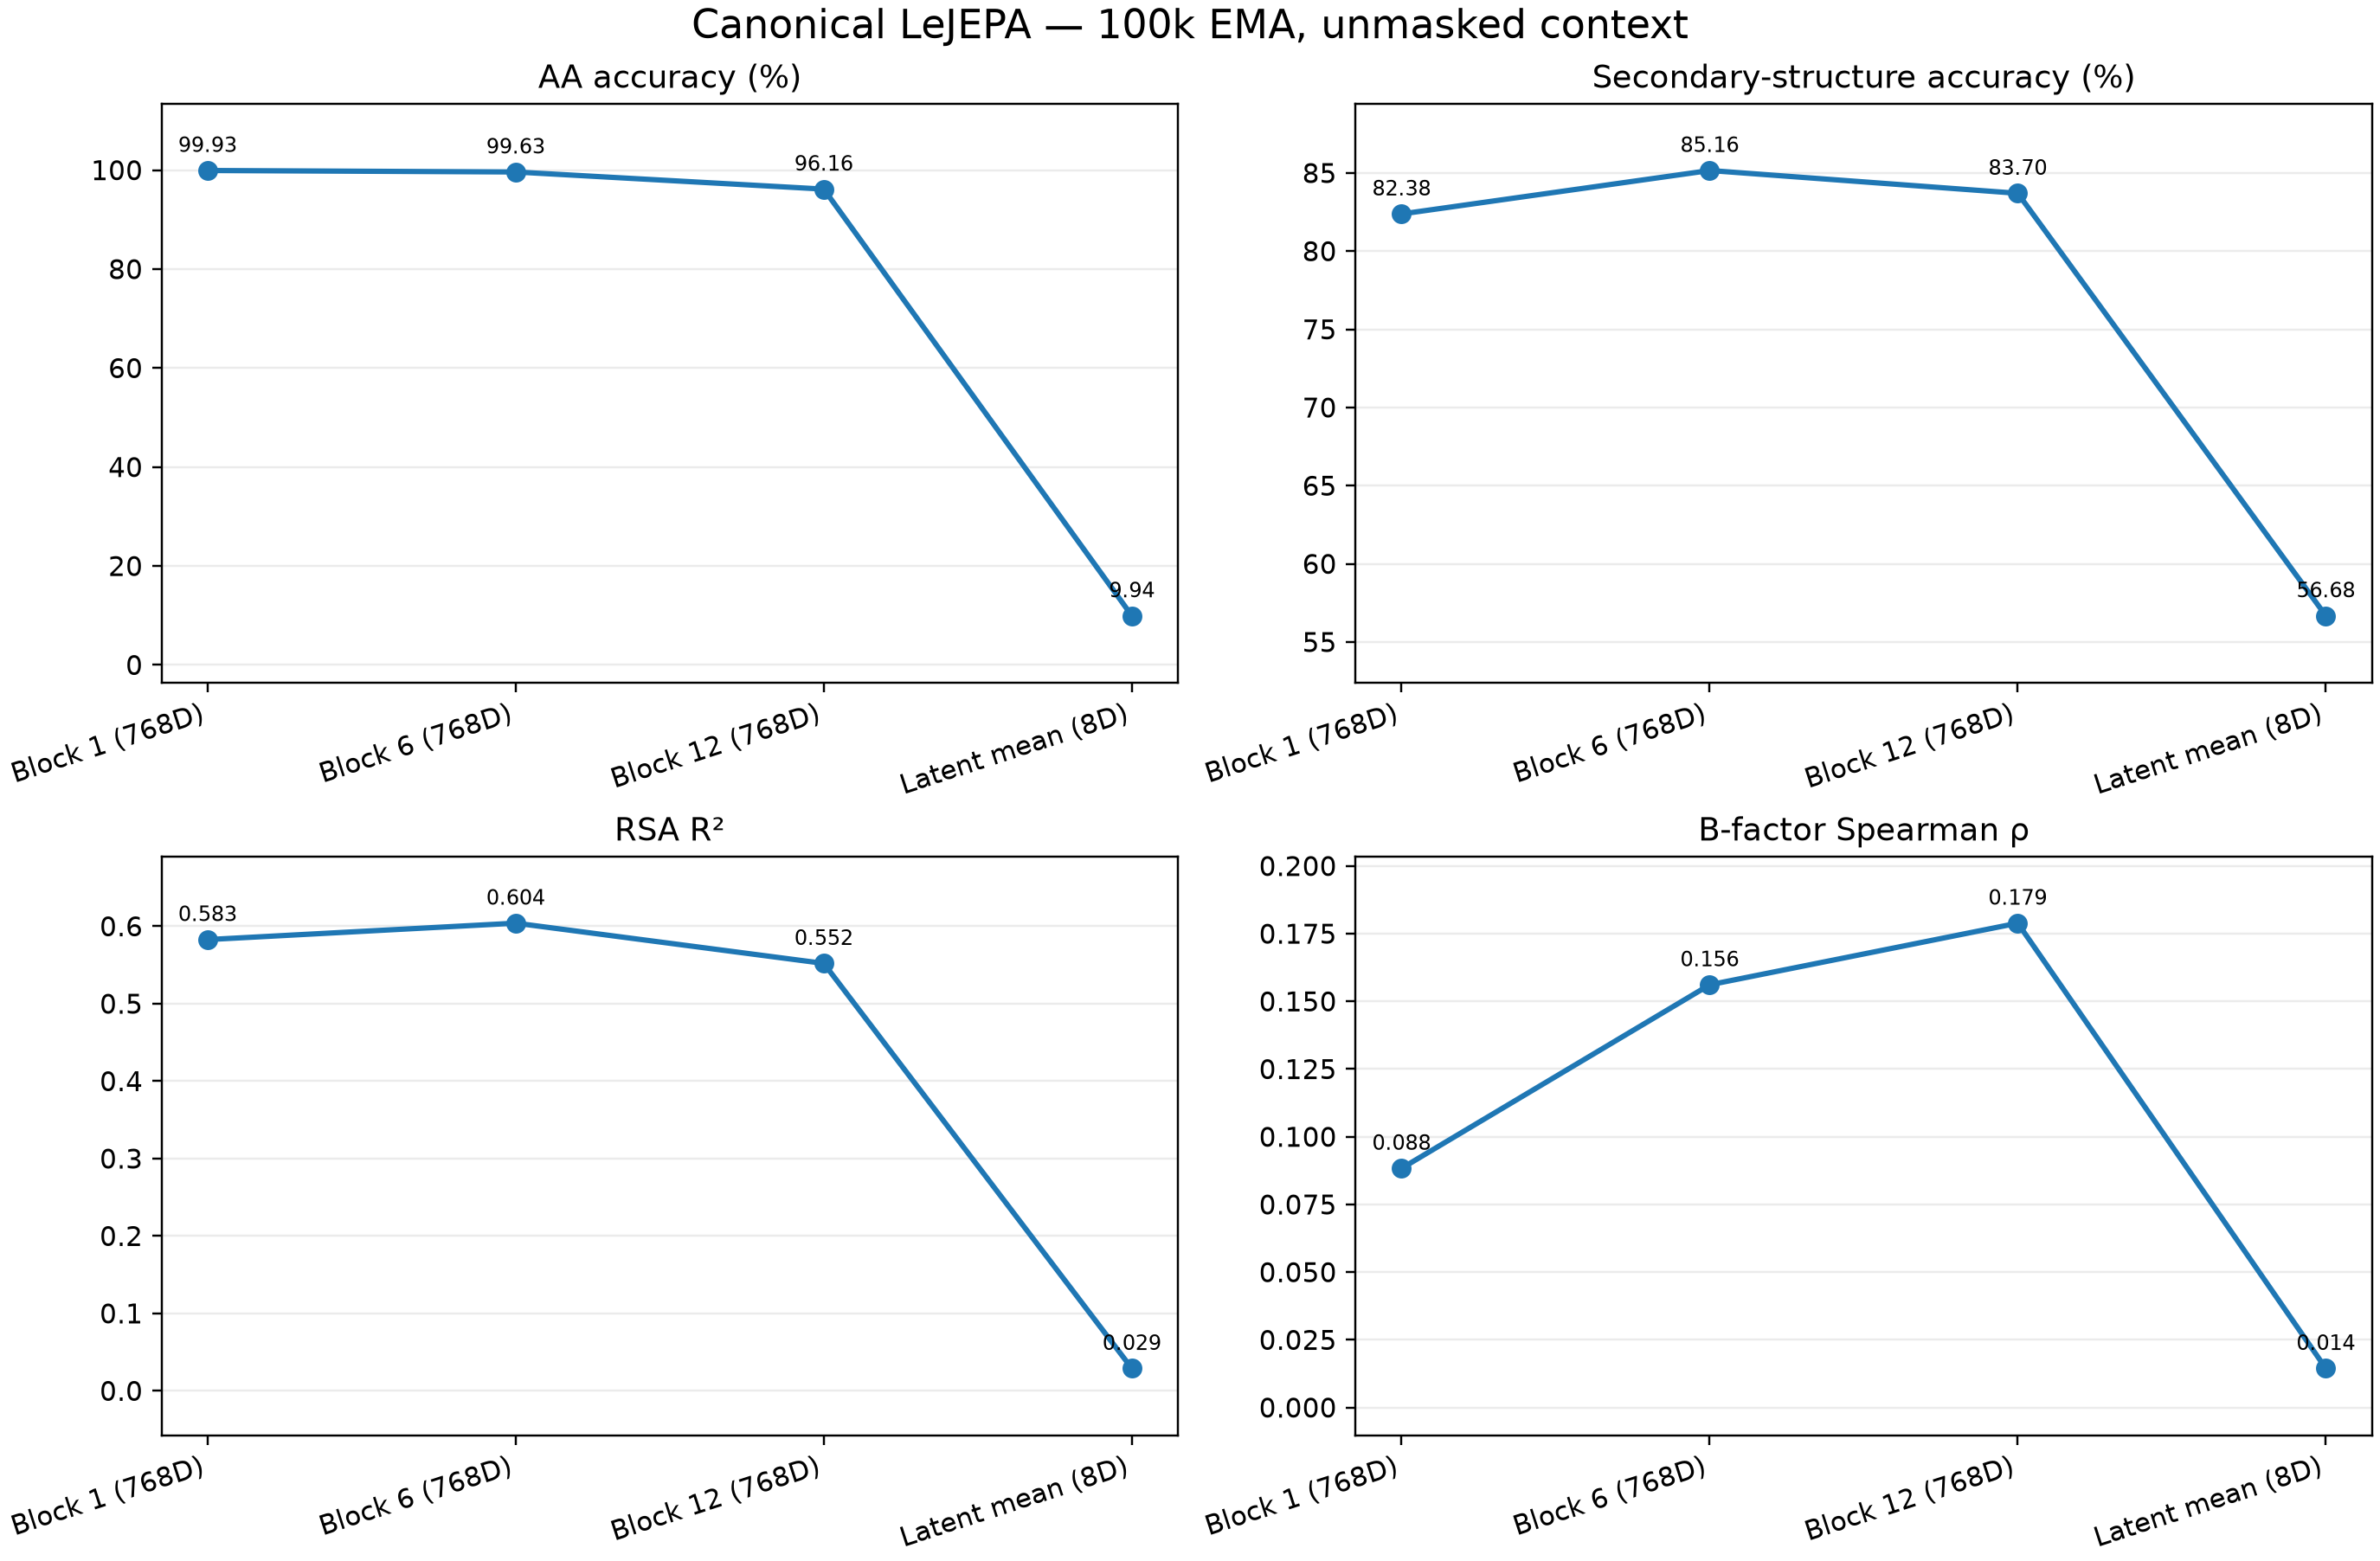
\includegraphics[width=\linewidth]{figures/results/canonical_lejepa_full_context_layerwise_probes.png}
\caption{Full-context linear probes from one uncropped LeJEPA 100k EMA checkpoint. Hidden states are 768D and the final latent mean is 8D. Block-1 SS and block-12 amino-acid/SS fits reported convergence warnings; the highlighted block-6 and latent-mean SS/RSA fits did not. Lines connect different readouts, not a training trajectory.}
\label{fig:results-layer-probes}
\end{figure}
\clearpage
%TC:endignore

% !TeX root = ../Project.tex
\section{Conclusion}
\label{sec:conclusion}

Finally, we summarise the contributions of this thesis, assess the limitations that affected the work and provide directions for future research.

\subsection{Summary of Contributions}

This thesis makes several contributions towards learning predictive representations of all-atom protein structures. First, we adapt JEPA, JEPA+SIGReg and LeJEPA to the La-Proteina encoder. These models introduce masked latent prediction and view alignment as alternatives to training the encoder through coordinate reconstruction. The three approaches also let us compare different collapse-prevention mechanisms, including an EMA target encoder and SIGReg with a shared encoder.

Second, we develop and test protein-specific choices for constructing the prediction problem. These include random, spatial and chemical masking, relative positional information, independent rotations, fixed-length crops and mutation actions. Through these experiments, we identify absolute residue-index and chain-length shortcuts and show how relative positions and cropping can reduce them. The rotation experiments further show that geometric augmentation can improve invariance without guaranteeing stronger downstream transfer. Together, these findings provide concrete guidance for designing protein views that remove unhelpful signals while retaining enough context for learning.

Third, we evaluate the learned representations from several complementary angles. StructTokenBench compares transfer across protein- and residue-level tasks, while linear probes, t-SNE visualisations, neighbour statistics and effective rank examine how the latent spaces are organised. Reconstruction tests ask whether information needed for recovering sequence and structure remains available. This combination separates downstream utility from properties such as high effective rank or visually distinct clusters, neither of which is sufficient on its own.

Finally, we examine where useful information is retained inside the encoder. Across blocks 1, 6 and 12 and the final latent, block 6 is the strongest readout for uncropped LeJEPA. Block 12 has the same 768-dimensional width, while the separately trained six-block encoder tests whether reducing depth reproduces the same benefit. These experiments establish intermediate readout selection as an important part of evaluating protein encoders rather than treating the final representation as the only available output. Thus, this work provides a tested set of JEPA-style adaptations and diagnostics for developing predictive all-atom protein models.

\subsection{Limitations}

The main limitations are that most configurations use one training run and that some cross-family comparisons differ in several design choices, limiting how directly the models can be compared. This section explains how these constraints affect the masking, layerwise, mutation and reconstruction findings.

\subsubsection{Model Comparisons}

The clearest comparisons in this thesis are within model families, where only the intended variable changes. These include the random-mask percentages and the absolute- versus relative-position variants. Comparisons across JEPA, JEPA+SIGReg and LeJEPA are less controlled because the methods differ in their objectives, encoder updates, regularisation, masks and readouts. While developing these models, we also encountered near-constant representations and effective rank close to one. We therefore adjusted masking and batch sizes to find a stable setting for each family. Cropping and discarding masked residues reduced memory use and allowed the LeJEPA models to use larger batches. 

Most configurations are represented by one training run. A complete one-GPU 100k training run requires approximately 16-20 GPU-hours, followed by 6-8 GPU-hours for full StructTokenBench evaluation. Each additional seed therefore costs approximately 22-28 GPU-hours. Repeating every comparison was outside the available compute budget, so small differences may reflect initialisation, sampling or optimisation noise. Targeted repeats of the main masking, positional and cropping comparisons would provide a useful uncertainty measurement.

\subsubsection{Masking and Cropping}

Our masking results are easiest to interpret when the remaining configuration is fixed. The random-mask sweep isolates masking percentage, while spatial masking changes both target shape and approximate coverage. The chemical masks use relative positions, removing the direct absolute-index shortcut from this comparison. However, the two objectives change both amino-acid visibility and which coordinates are hidden, so their difference cannot be attributed to one factor alone.

Cropping required a similar compromise. The matched 20/80 control shows that cropping itself reduces chain-length organisation, but its effective rank falls to $1.61/8$. With only around ten visible residues in each 48-residue local crop, this setting appears too difficult for the shorter view. We therefore use 20/50 masking in the reported cropped models, leaving around 24 local residues visible and obtaining near-full effective rank. That model also uses a larger batch, so these results motivate the selected setting without isolating masking percentage as the cause of the higher scores. Other crop lengths, mask ratios and spatially defined crops remain unexplored.

\subsubsection{Downstream and Representation Evaluation}

The evaluation covers complementary properties, but no single measurement establishes representation quality. StructTokenBench spans local functional sites, flexibility and protein-level remote homology, but conclusions from one benchmark may not generalise to other datasets. The task-wise results reveal that the strongest model depends on the biological scale and property being measured, but different labels and metrics prevent a meaningful aggregate ranking of residue- versus protein-level performance. Evaluation on additional structure and function benchmarks would test whether these task-specific profiles persist, as proposed in Section~\ref{sec:future-work}.

Linear probes measure linearly accessible information rather than everything a nonlinear predictor could recover. The randomly initialised encoder also exposes amino-acid identity because residue identity is part of its input, so probe performance does not always reflect information learned during training. t-SNE and neighbour purity can make organisation and shortcuts visible, but do not show that a downstream predictor relies on those neighbourhoods. Effective rank detects concentration into a small number of directions, but does not measure whether those directions contain useful biological information. For this reason, we base the main interpretations on agreement between downstream transfer, probes and latent-space diagnostics rather than a change in one measurement alone.

\subsubsection{Intermediate Layers}

The layerwise study covers selected readouts from only two trained encoders because every block requires a separate downstream evaluation. We evaluate blocks 1, 6 and 12 rather than every layer, so we cannot establish that block 6 is the optimal readout or determine where different structural and functional properties first become accessible. Block 12 has the same 768-dimensional width as block 6 and is weaker, which shows that width alone is not sufficient. However, comparisons with the final representation still change both encoder stage and dimensionality.

The separately trained six-block encoder addresses a different question. It shows that reading block 6 from the twelve-block encoder is not equivalent to training a shorter network, but one model cannot establish how encoder depth affects this behaviour more generally. Further experiments are needed to determine whether the middle-layer advantage persists across architectures and which biological information is gained or lost through later blocks.

\subsubsection{Mutation Conditioning}

Mutation conditioning remains an initial proposal for introducing actions into all-atom JEPA training. The current objective changes one residue identity while retaining the original coordinates because the relaxed mutant conformation is unknown. The downstream evaluation therefore cannot establish that the model predicts realistic structural, stability or functional consequences. The present experiments cover only single substitutions sampled uniformly, leaving biologically possible mutations and combinations of mutations unexplored.

\subsubsection{Reconstruction and Generation}
\label{sec:limitations-reconstruction}

There are several key differences between the baseline and JEPA reconstruction pipelines. First, the baseline encoder and decoder are trained jointly to reconstruct the protein, so its latent is explicitly optimised for sequence and coordinate recovery. The JEPA encoder is instead trained to predict latent representations. Although all-atom coordinates are part of its input, its learning signal remains in latent space and never includes a coordinate-reconstruction loss. We freeze this encoder and fit the decoder afterwards, making reconstruction a new task rather than the encoder's original objective. Second, the baseline decoder receives a sampled VAE latent, while the JEPA decoder receives the deterministic latent mean. These differences limit what can be concluded from a direct comparison of their reconstruction scores.

\subsection{Future Work}
\label{sec:future-work}

Building on these limitations, the next steps are to strengthen the central comparisons, further examine intermediate representations, and extend their use to mutation prediction, generation and protein dynamics.

\subsubsection{Scaling and Training}

With more compute, the next step is to repeat the central comparisons across training seeds and extend the mask and crop sweeps. Random, spatial and chemical masks should cover a wider range of percentages. Larger stable batches would help separate objective behaviour from optimisation noise. Testing additional crop lengths and local-mask ratios would show how much sequence context each view requires. Spatial crops defined by a three-dimensional radius would provide another test of whether structural neighbourhoods form better views than contiguous sequence windows. Longer training and broader comparisons of encoder depth and latent width would show whether the observed patterns persist with scale. Another experiment could initialise the encoder from the La-Proteina autoencoder and then fine-tune it with a JEPA objective. This would test whether predictive learning can reorganise an atomically informative representation without learning it from scratch. The resulting models should also be evaluated on additional structure and function benchmarks such as ATOM3D and TAPE to test whether their task-specific strengths extend beyond StructTokenBench \citep{townshend2020atom3d,rao2019tape}.

\subsubsection{Selecting Intermediate Representations}

The intermediate-layer results motivate a systematic sweep across every encoder block, model size and downstream task. Following the layerwise probing approach of \citet{joeres2026taskdataset}, the same task-specific probe could be trained on each frozen block and its performance plotted across depth. This would show where each property is most accessible and how its signal changes through the encoder. If the pattern remains, an early-exit method such as that proposed for protein language models by \citet{hart2026protein} could improve both prediction and inference efficiency.

\subsubsection{Exploring Mutations}

A more ambitious extension is to use latent prediction to explore which mutations preserve or improve protein properties. Evolutionary amino-acid preferences, following the motivation of EvoRank \citep{gong2024evorank}, could replace uniform substitutions with plausible actions. Relaxed mutant structures would provide targets for conformational changes, while stability and function measurements would test whether the predicted consequences are useful. Extending the objective to several coordinated substitutions could eventually move from representing known proteins towards exploring new sequences under structural and functional constraints.

\subsubsection{Generation and Conformational Dynamics}

Future work should first improve reconstruction from JEPA latents. A decoder that enforces valid residue geometry could reduce compressed residues and atomic overlaps. Reconstruction without native C$\alpha$ anchors would then test whether the latent preserves the complete structure rather than only the atoms around a known backbone. Following La-Proteina, latent perturbation experiments could vary individual residue embeddings and measure whether the decoded changes remain local or propagate to structurally connected residues \citep{la-proteina}. These experiments would show whether the learned space supports controlled structural changes before using it for protein generation.

Inspired by SLAE, future work could evaluate conformational trajectories using multiple conformations of the same protein, ideally ordered frames from a molecular dynamics simulation \citep{chen2026slae}. We could test whether neighbouring frames remain close in latent space and whether latent distance follows structural change along the trajectory. Proteins with well-characterised open and closed conformations could provide motion trajectories. Interpolating between trajectory embeddings and decoding the intermediate points would then test whether the latent space supports gradual structural changes.

\subsection{Conclusion}

This thesis adapts JEPA and LeJEPA objectives to residue-level all-atom protein structures and develops a framework for examining what their representations learn. The experiments show that predictive learning can support both downstream transfer and detailed latent-space analysis, while exposing shortcuts caused by position, chain length and view construction. Relative positions, fixed-length crops and rotation augmentation provide concrete ways to modify these signals, and the layerwise study shows that valuable information may remain inside the encoder rather than in its final output.

The adaptations and diagnostics developed here identify which design choices work, where they fail and what information the resulting representations retain. Future work should extend these representations towards protein dynamics, richer mutation experiments and generation, while studying more deeply how information changes across the encoder. By adapting JEPA-style learning to all-atom protein structures, this thesis contributes one step towards protein world models with a focus on representation learning.

%\section{Conclusion}
\label{sec:conclusion}

\subsection{Summary}

[ ] Summarise the motivation and objectives of this work.

[ ] Summarise the proposed methods and experimental findings.

[ ] State the main conclusions and answer the research questions.

\subsection{Contributions}

[ ] Summarise the main scientific and technical contributions of this thesis.

[ ] Highlight the key findings.

\subsection{Future Work}

[ ] Investigate larger latent representations and model architectures.

[ ] Explore alternative masking strategies and predictive learning objectives.

[ ] Evaluate on additional downstream benchmarks and larger datasets.

[ ] Extend action-conditioned representation learning to more complex biological perturbations.

% %%%% REFERENCES

{\setlength{\baselineskip}{0pt} % JEM: Single-space References
\renewcommand*\MakeUppercase[1]{#1}
	\printbibliography[heading=bibintoc,title={\bibtitle}]}

\clearpage
\startappendices
% !TeX root = ../Project.tex
\section{JEPA+SIGReg Architecture}
\label{app:jepa-sigreg-architecture}

\begin{figure}[htbp]
\centering
\includegraphics[width=\linewidth]{figures/methods/JEPA_SIGReg.pdf}
\caption{JEPA+SIGReg architecture. A shared encoder processes the masked context and complete target views, while a cross-attention predictor predicts the selected target-residue latents. Training combines the prediction loss with SIGReg.}
\label{fig:methods-jepa-sigreg-architecture}
\end{figure}

\clearpage
% !TeX root = ../Project.tex
\section{Downstream Results for Proteins up to 256 Residues}
\label{app:l256}
Table~\ref{tab:results-stb-l256} reports StructTokenBench results for proteins with at most 256 residues.
\begingroup
\ifdefined\stbworkshopbox\else\newsavebox{\stbworkshopbox}\fi
\providecommand{\stbworkshopfit}{\ifdim\wd\stbworkshopbox>\linewidth\resizebox{\linewidth}{!}{\usebox{\stbworkshopbox}}\else\usebox{\stbworkshopbox}\fi}
\begin{table}[H]
\centering
\resultstableformat
\setlength{\tabcolsep}{3pt}
\renewcommand{\arraystretch}{0.92}
\captionsetup{font=small,skip=5pt}
\fontsize{8.5}{10}\selectfont
\caption{StructTokenBench evaluation restricted to proteins with at most 256 residues.}
\label{tab:results-stb-l256}
\sbox{\stbworkshopbox}{%
\begin{tabular}{@{}lllrrrrrrrr@{}}
\toprule
\multirow{2}{*}{Task type} & \multirow{2}{*}{Task} & \multirow{2}{*}{Split} & \multicolumn{2}{c}{Autoencoders} & \multicolumn{3}{c}{JEPA} & \multicolumn{3}{c}{JEPA+SIGReg} \\[1.8pt]
 & & & $C_\alpha$ & Full AE & 50\% & 70\% & Mut. & 50\% & 70\% & Mut. \\
\midrule
\multicolumn{11}{c}{\textbf{Functional-site prediction: AUROC $\times100$}} \\
\midrule
\multirow{5}{*}{Binding site} & \multirow{2}{*}{BindInt} & Fold & 41.69 & 40.66 & 40.54 & 42.03 & \textbf{42.14} & 38.91 & 40.65 & 39.69 \\
 &  & SF & 86.84 & 85.80 & 87.39 & 86.07 & 86.82 & \textbf{89.52} & 83.70 & 88.85 \\
 & \multirow{2}{*}{BindBio} & Fold & 62.96 & \textbf{65.32} & 55.60 & 58.54 & 57.47 & 57.12 & 57.47 & 57.16 \\
 &  & SF & 63.23 & \textbf{65.63} & 58.22 & 60.02 & 59.49 & 59.60 & 59.79 & 59.73 \\
 & BindShake & Test & 59.19 & \textbf{65.11} & 53.76 & 64.42 & 63.89 & 59.73 & 59.96 & 60.83 \\
\multirow{4}{*}{Catalytic site} & \multirow{2}{*}{CatInt} & Fold & 58.97 & \textbf{61.19} & 58.92 & 58.09 & 59.94 & 59.38 & 58.19 & 57.39 \\
 &  & SF & 76.50 & \textbf{76.82} & 73.79 & 75.37 & 75.36 & 74.33 & 75.91 & 76.47 \\
 & \multirow{2}{*}{CatBio} & Fold & 64.01 & \textbf{71.89} & 54.46 & 62.41 & 60.40 & 53.05 & 51.54 & 51.53 \\
 &  & SF & 78.31 & \textbf{84.44} & 65.48 & 71.96 & 69.87 & 62.06 & 61.68 & 63.21 \\
\multirow{2}{*}{Conserved site} & \multirow{2}{*}{Con} & Fold & 57.20 & \textbf{59.98} & 59.51 & 58.51 & 59.34 & 58.85 & 59.43 & 59.22 \\
 &  & SF & 71.97 & 73.48 & 70.73 & 71.22 & 72.43 & \textbf{74.30} & 74.10 & 74.11 \\
\multirow{2}{*}{Repeat motif} & \multirow{2}{*}{Rep} & Fold & 65.38 & 64.43 & 66.08 & 65.91 & 65.37 & \textbf{67.73} & 66.97 & 67.08 \\
 &  & SF & 80.79 & 79.82 & \textbf{82.00} & 79.24 & 81.25 & 77.65 & 76.02 & 77.46 \\
\multirow{2}{*}{Epitope region} & \multirow{2}{*}{Ept} & Fold & 56.28 & 55.21 & \textbf{59.29} & 54.79 & 56.57 & 58.34 & 56.67 & 55.90 \\
 &  & SF & 64.15 & 62.59 & \textbf{65.09} & 60.61 & 61.86 & 61.02 & 60.76 & 57.63 \\
\midrule
\multicolumn{11}{c}{\textbf{Remote homology: macro-F1 $\times100$}} \\
\midrule
\multirow{3}{*}{Remote homology} & \multirow{3}{*}{Homo} & Fold & 7.89 & 6.29 & 7.10 & \textbf{10.21} & 8.77 & 7.43 & 7.98 & 8.54 \\
 &  & Family & \textbf{35.26} & 26.86 & 17.67 & 21.29 & 17.00 & 21.52 & 20.01 & 26.60 \\
 &  & SF & 8.41 & 10.47 & 4.97 & \textbf{11.59} & 8.51 & 7.73 & 6.67 & 6.14 \\
\midrule
\multicolumn{11}{c}{\textbf{Structural flexibility: Spearman's $\rho\times100$}} \\
\midrule
\multirow{6}{*}{Flexibility} & \multirow{2}{*}{FlexRMSF} & Fold & 14.98 & \textbf{45.34} & 26.50 & 30.46 & 30.76 & 12.12 & 10.48 & 10.31 \\
 &  & SF & 13.96 & \textbf{44.34} & 31.68 & 28.47 & 33.10 & 10.26 & 10.24 & 8.45 \\
 & \multirow{2}{*}{FlexBFactor} & Fold & 11.21 & \textbf{26.00} & 1.80 & 19.62 & 16.25 & 1.91 & 3.32 & 2.80 \\
 &  & SF & 11.26 & \textbf{26.94} & 12.97 & 22.10 & 23.40 & 4.01 & 3.56 & 4.92 \\
 & \multirow{2}{*}{FlexNEQ} & Fold & 15.98 & 24.95 & 10.52 & \textbf{33.38} & 16.92 & 7.98 & 7.75 & 7.80 \\
 &  & SF & 13.51 & 22.11 & 11.43 & \textbf{29.19} & 10.87 & 6.61 & 6.82 & 6.63 \\
\bottomrule
\end{tabular}%
}
\stbworkshopfit
\end{table}

\clearpage
\endgroup

% !TeX root = ../Project.tex
\section{Supporting Result Diagnostics}
\label{sec:results-supporting}

Figures~\ref{fig:appendix-reconstruction-examples} and~\ref{fig:appendix-reconstruction-failures} show additional whole-protein reconstructions and representative local failure modes.

\begin{figure}[H]
\centering
\captionsetup{font=small,skip=3pt}
\begin{minipage}[t]{0.48\linewidth}
  \centering
  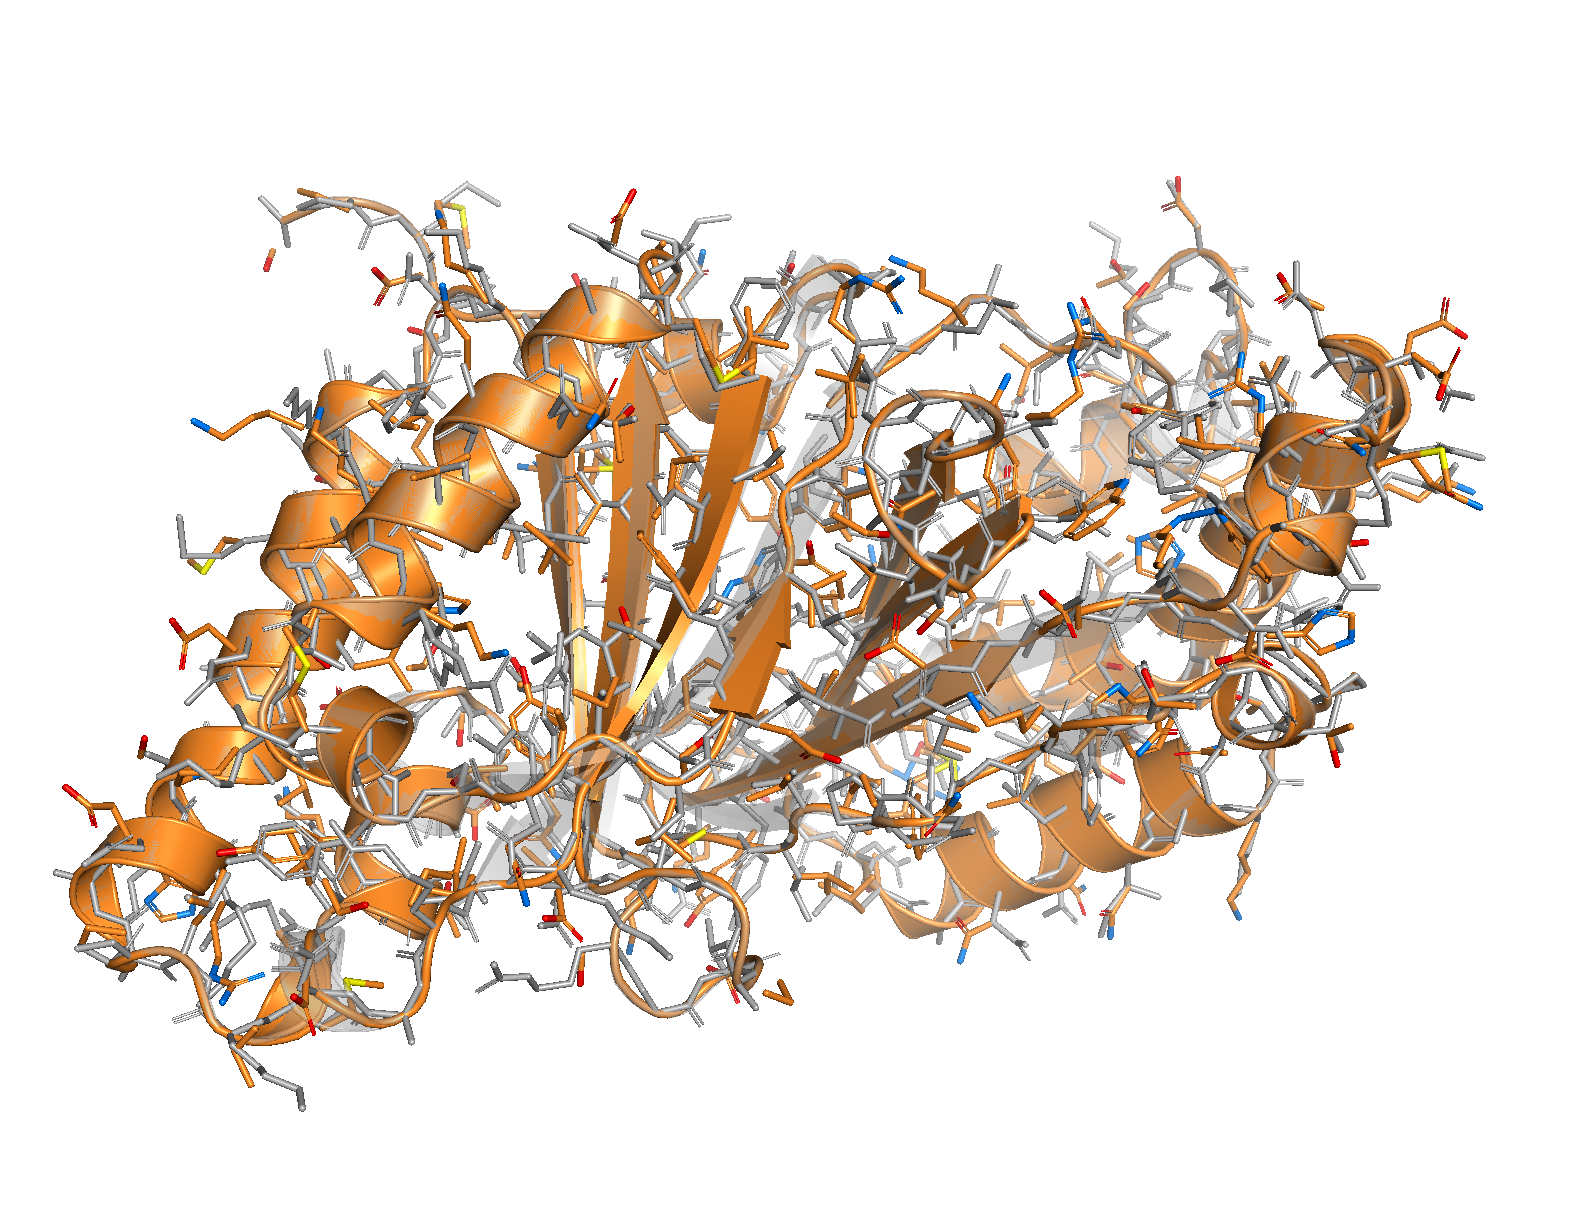
\includegraphics[height=0.14\textheight]{figures/protein_figures/5a13_G.png}\\[-2pt]
  \small (a) 5A13 chain G
\end{minipage}\hfill
\begin{minipage}[t]{0.48\linewidth}
  \centering
  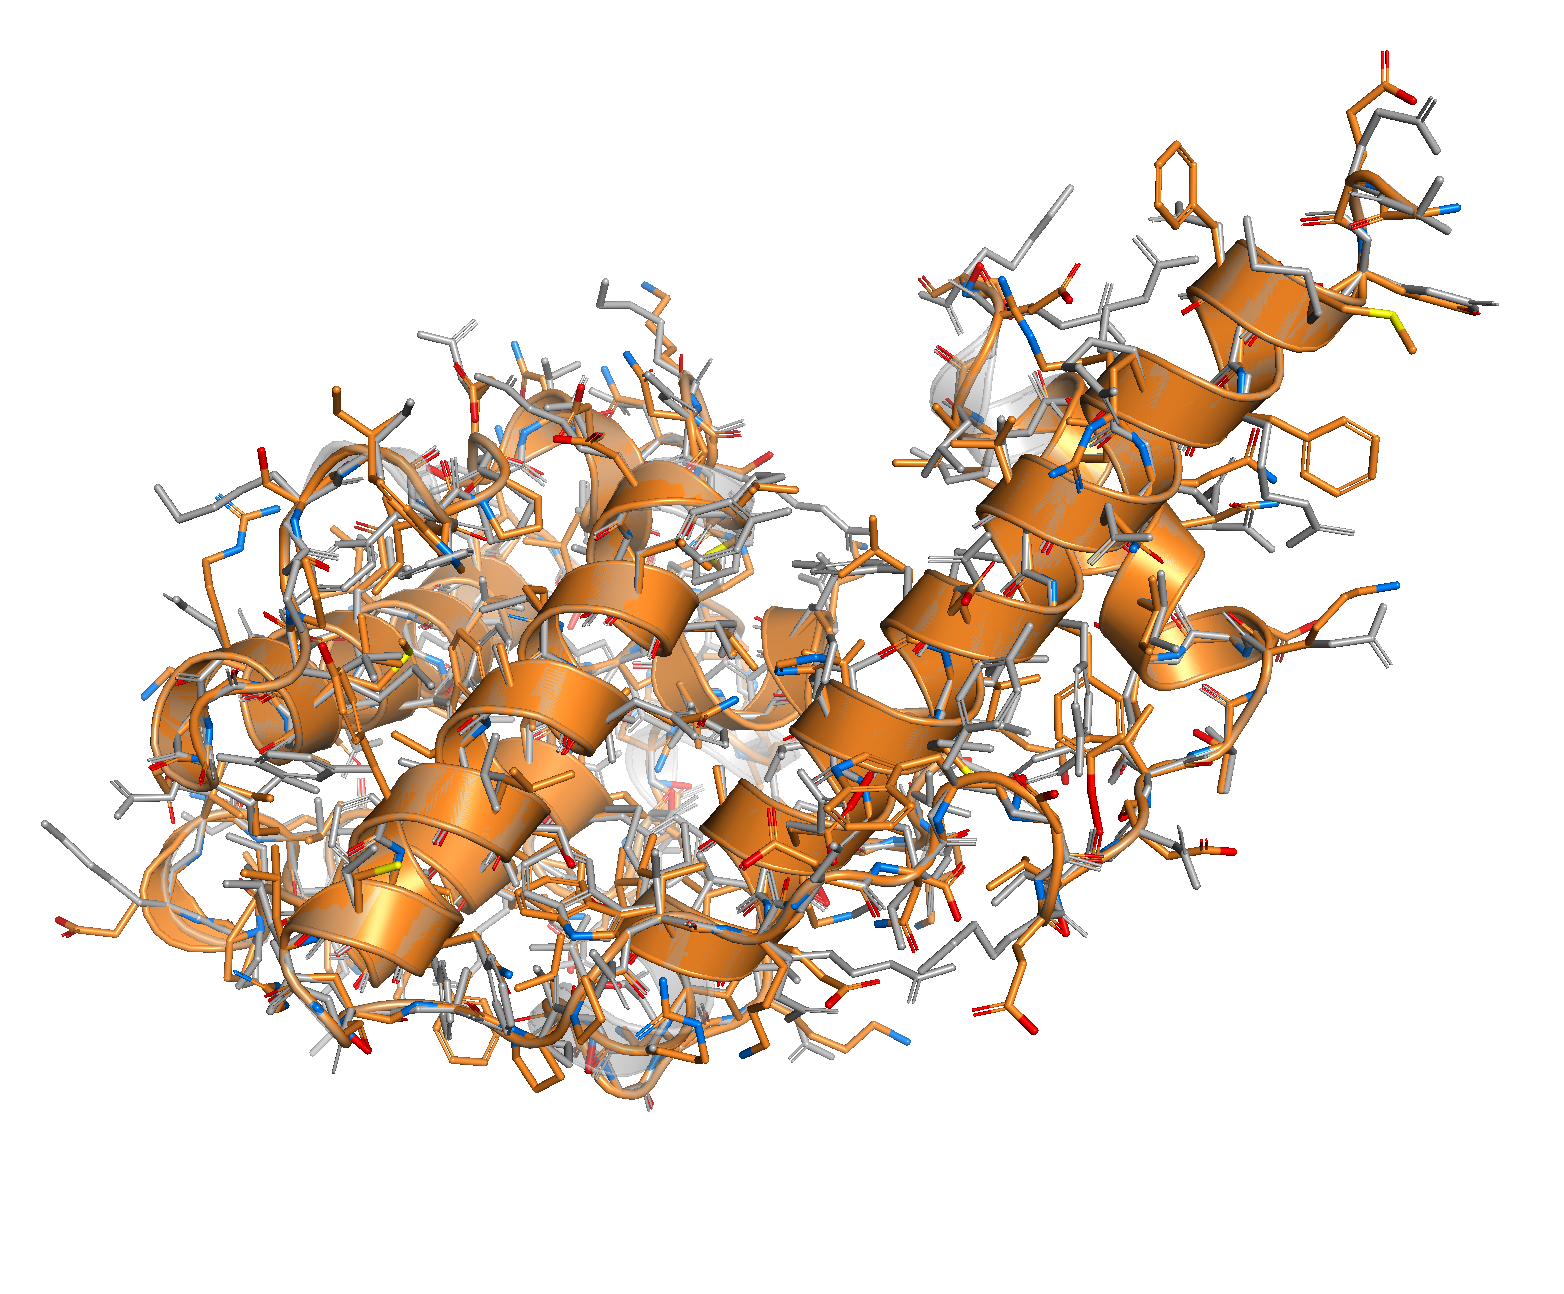
\includegraphics[height=0.14\textheight]{figures/protein_figures/5l0o_A.png}\\[-2pt]
  \small (b) 5L0O chain A
\end{minipage}

\vspace{2pt}
\begin{minipage}[t]{0.48\linewidth}
  \centering
  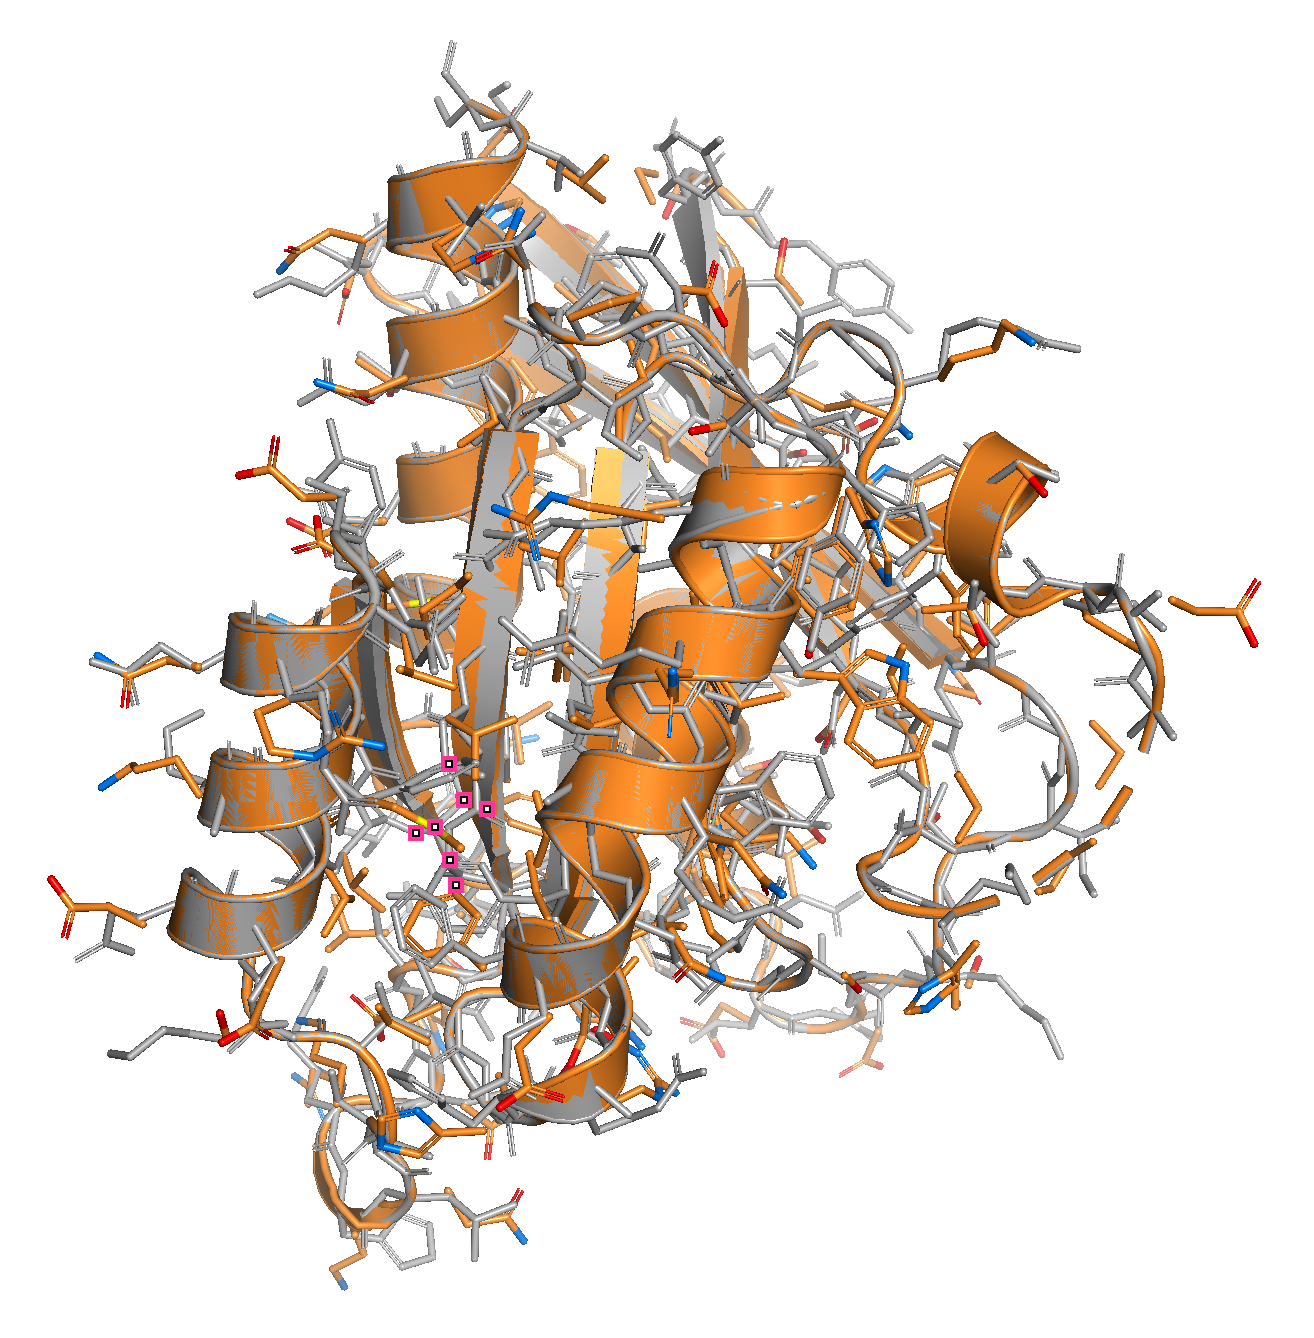
\includegraphics[height=0.14\textheight]{figures/protein_figures/5xr7_A.png}\\[-2pt]
  \small (c) 5XR7 chain A
\end{minipage}\hfill
\begin{minipage}[t]{0.48\linewidth}
  \centering
  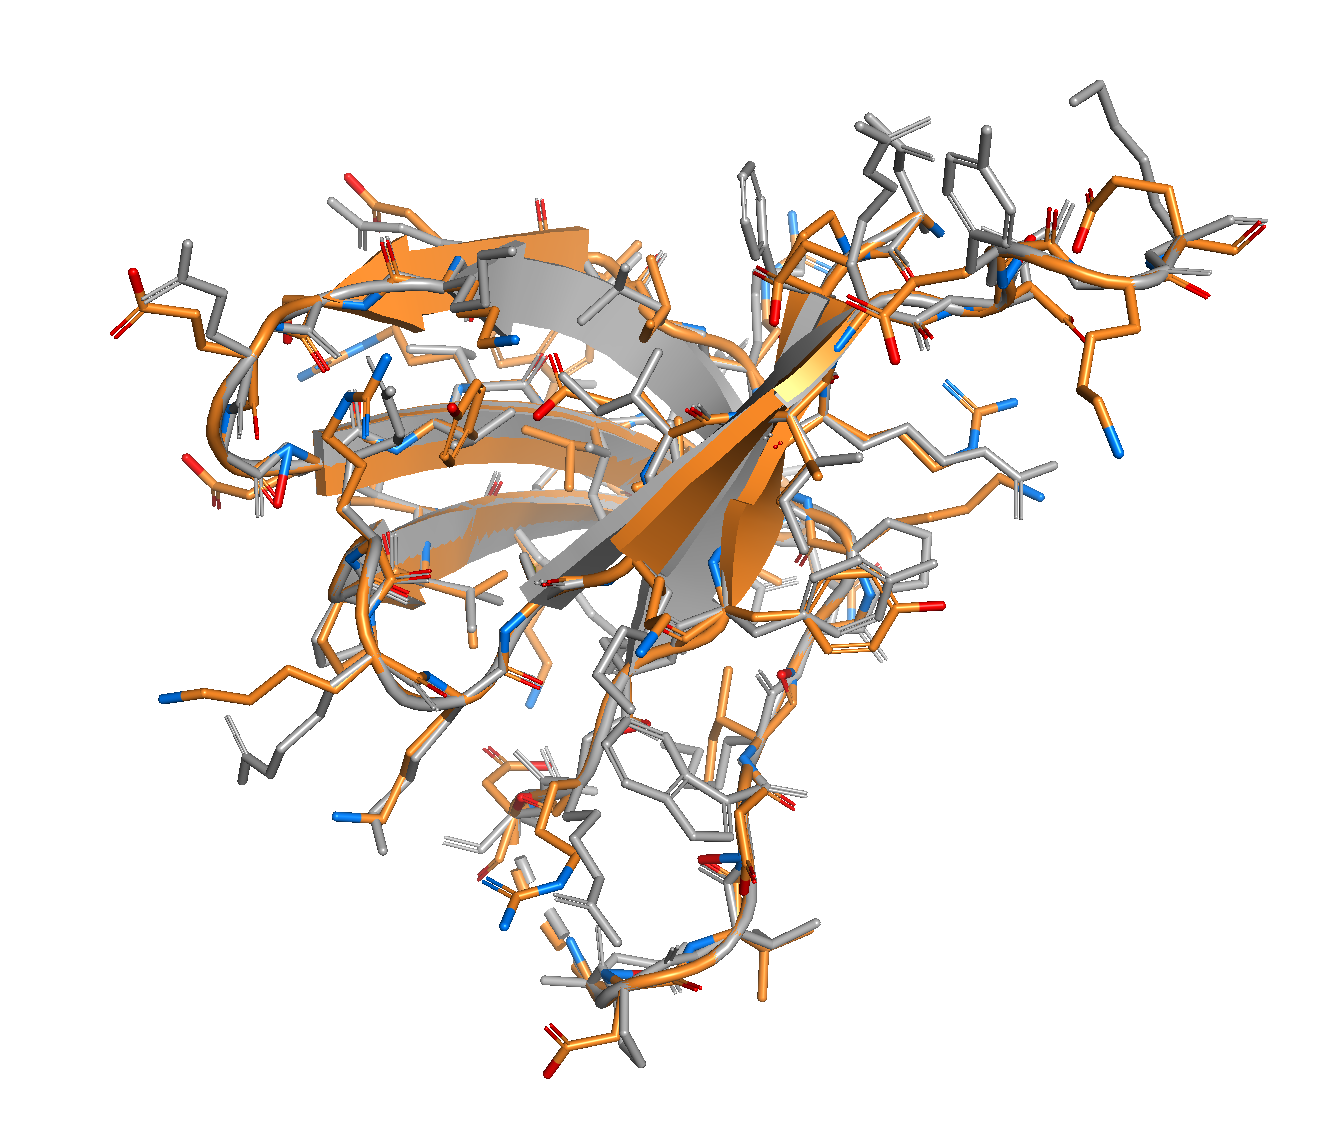
\includegraphics[height=0.14\textheight]{figures/protein_figures/8cbv_A.png}\\[-2pt]
  \small (d) 8CBV chain A
\end{minipage}
\caption{Whole-protein overlays of native structures in grey and postprocessed JEPA reconstructions in orange.}
\label{fig:appendix-reconstruction-examples}
\end{figure}

\begin{figure}[H]
\centering
\captionsetup{font=small,skip=3pt}
\begin{minipage}[t]{0.48\linewidth}
  \centering
  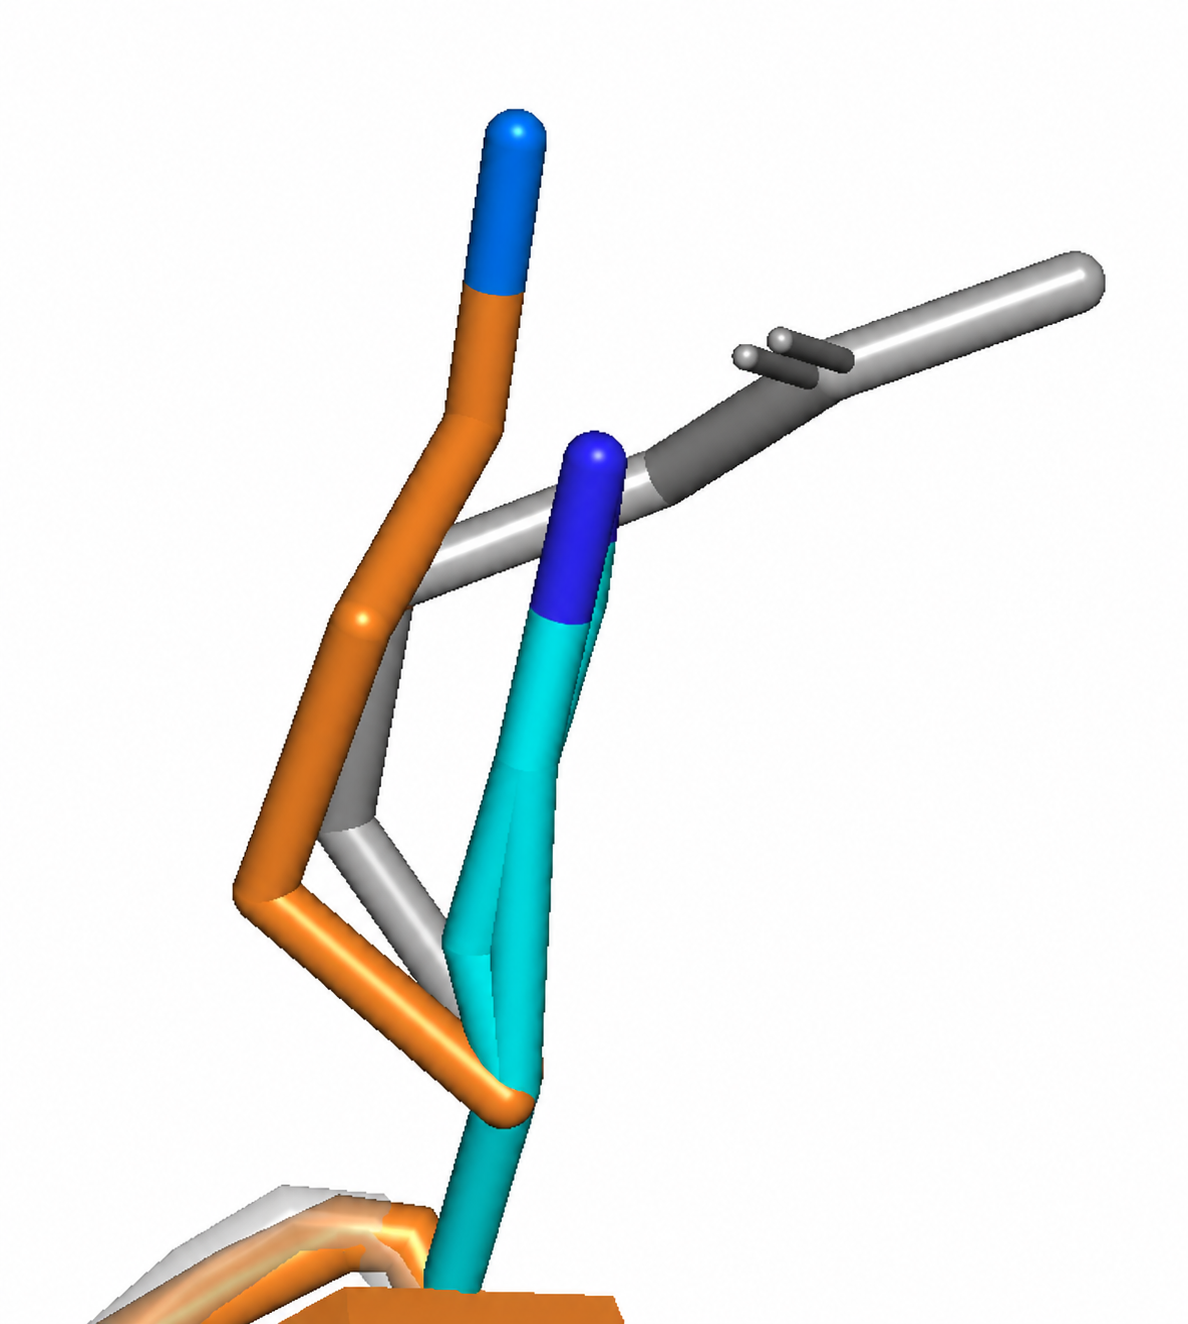
\includegraphics[height=0.14\textheight]{figures/protein_figures/fm1-clean.png}\\[-2pt]
  \small (a) Distorted bond geometry
\end{minipage}\hfill
\begin{minipage}[t]{0.48\linewidth}
  \centering
  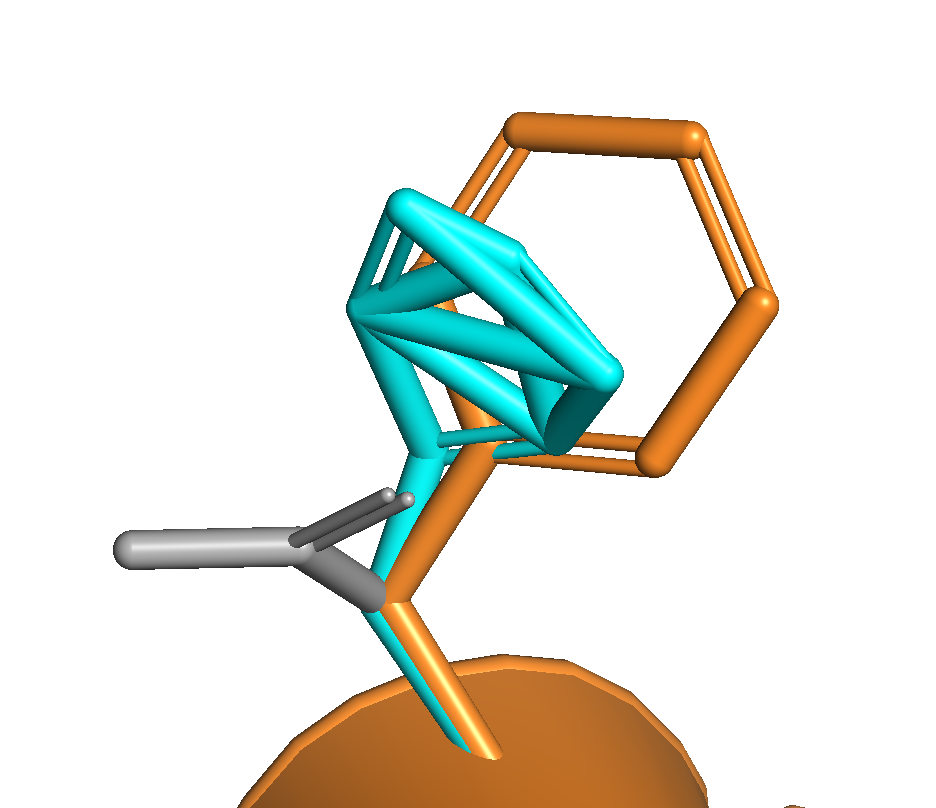
\includegraphics[height=0.14\textheight]{figures/protein_figures/fm2.png}\\[-2pt]
  \small (b) Overlapping side-chain atoms
\end{minipage}

\vspace{2pt}
\begin{minipage}[t]{0.48\linewidth}
  \centering
  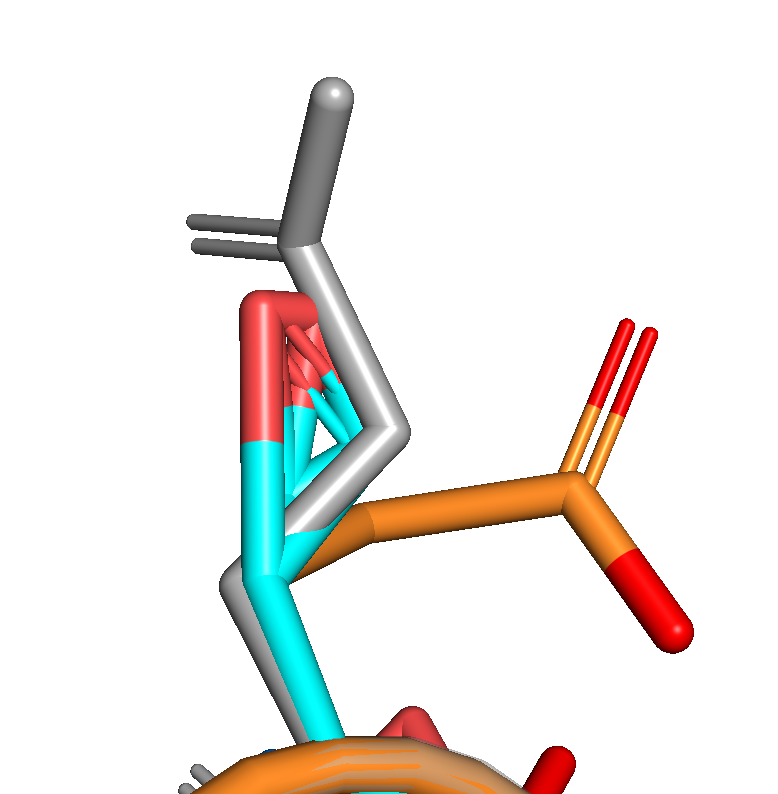
\includegraphics[height=0.14\textheight]{figures/protein_figures/fm3.png}\\[-2pt]
  \small (c) Misplaced side-chain atoms
\end{minipage}\hfill
\begin{minipage}[t]{0.48\linewidth}
  \centering
  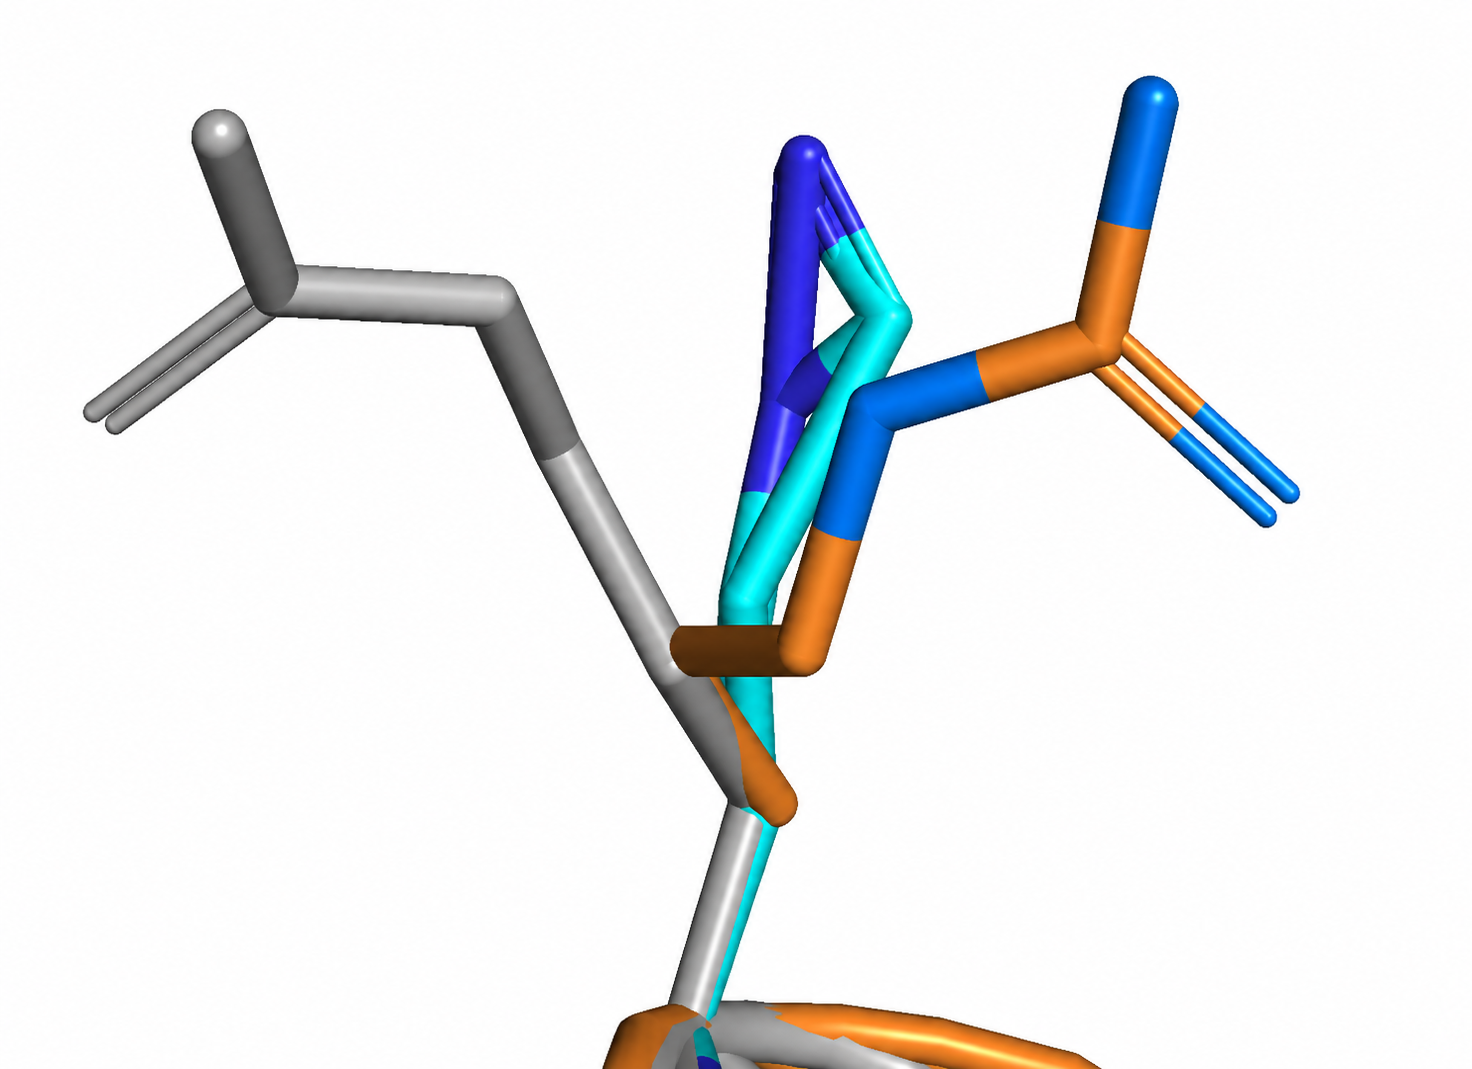
\includegraphics[height=0.14\textheight]{figures/protein_figures/fm4-clean.png}\\[-2pt]
  \small (d) Distorted local connection
\end{minipage}
\caption{Examples of local geometric failure modes. Native structures are grey, postprocessed JEPA predictions are orange, and direct decoder outputs are cyan.}
\label{fig:appendix-reconstruction-failures}
\end{figure}


\clearpage
\section{Latent-Space Model and Design Comparisons}
\label{app:latent-figures}

\begin{figure}[H]
\centering
\captionsetup{font=small,skip=3pt}
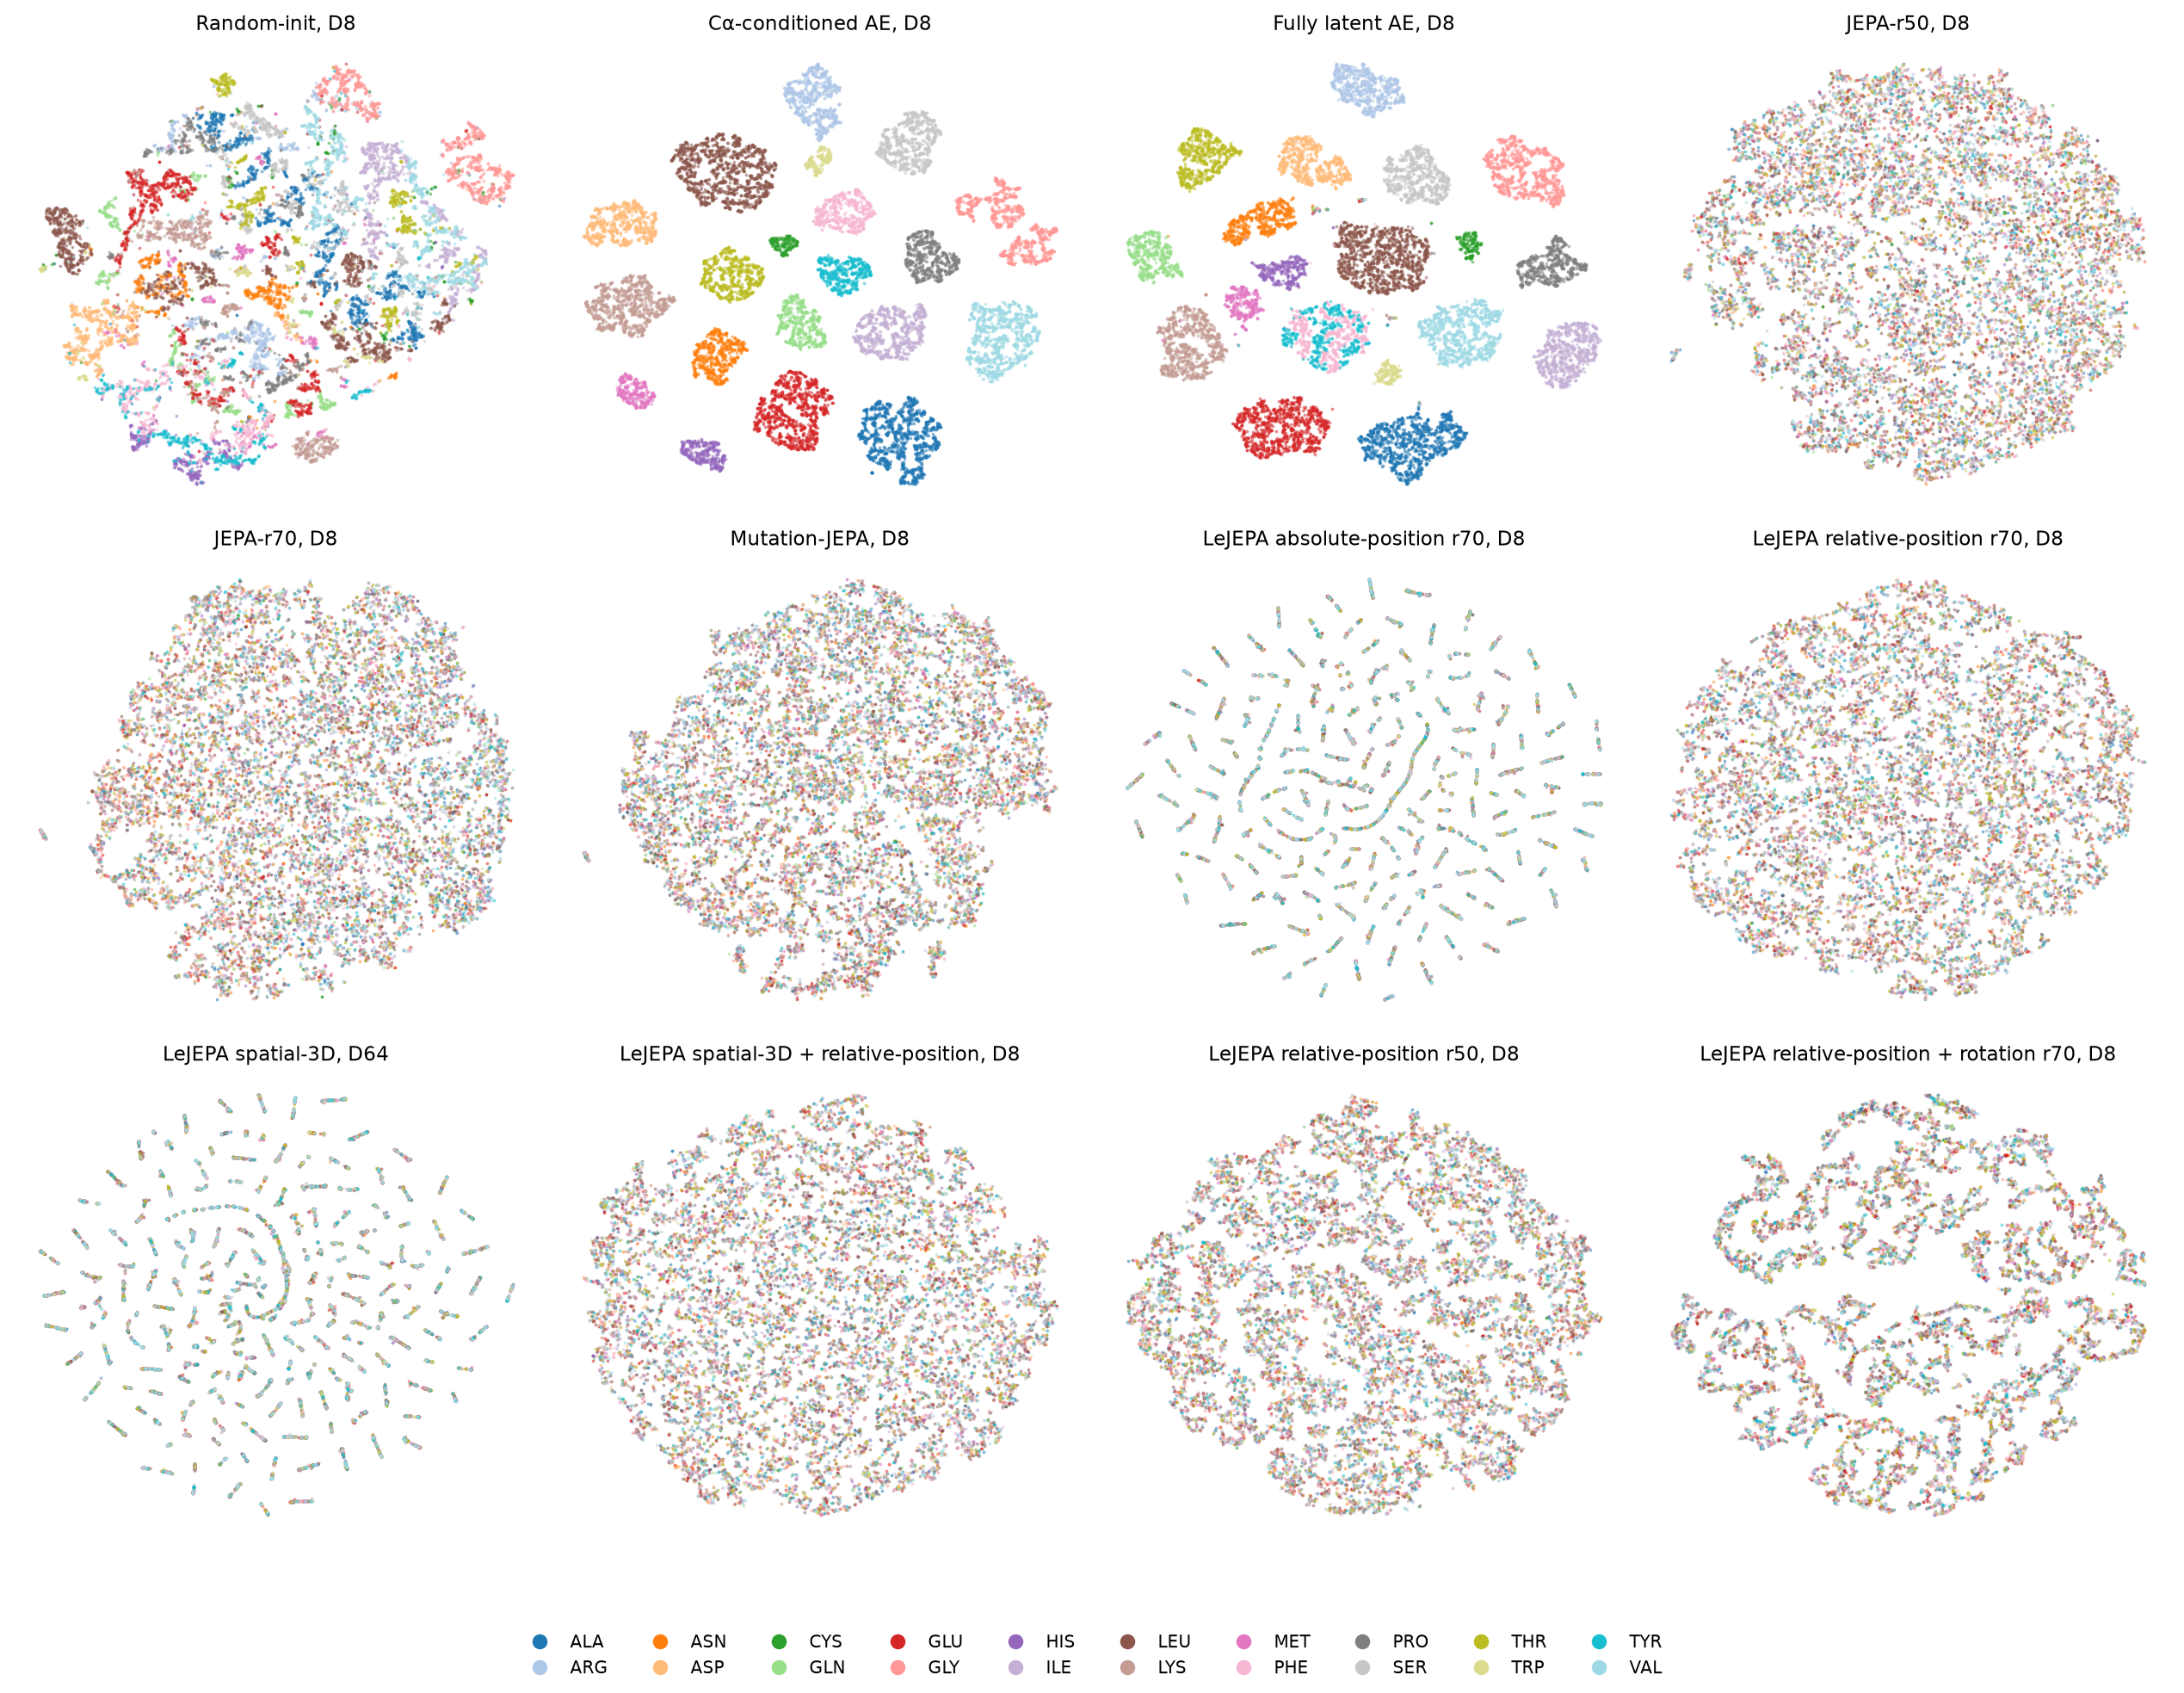
\includegraphics[width=\linewidth]{figures/results/tsne_full12_exact.png}
\caption{Per-residue t-SNE for the full 100k model roster, coloured by amino-acid identity. The same evaluation residues and visualisation settings are used across models. This figure provides qualitative latent-space context for the main L600 results.}
\label{fig:full-latent-grid}
\end{figure}

\begin{figure}[H]
\centering
\captionsetup{font=small,skip=3pt}
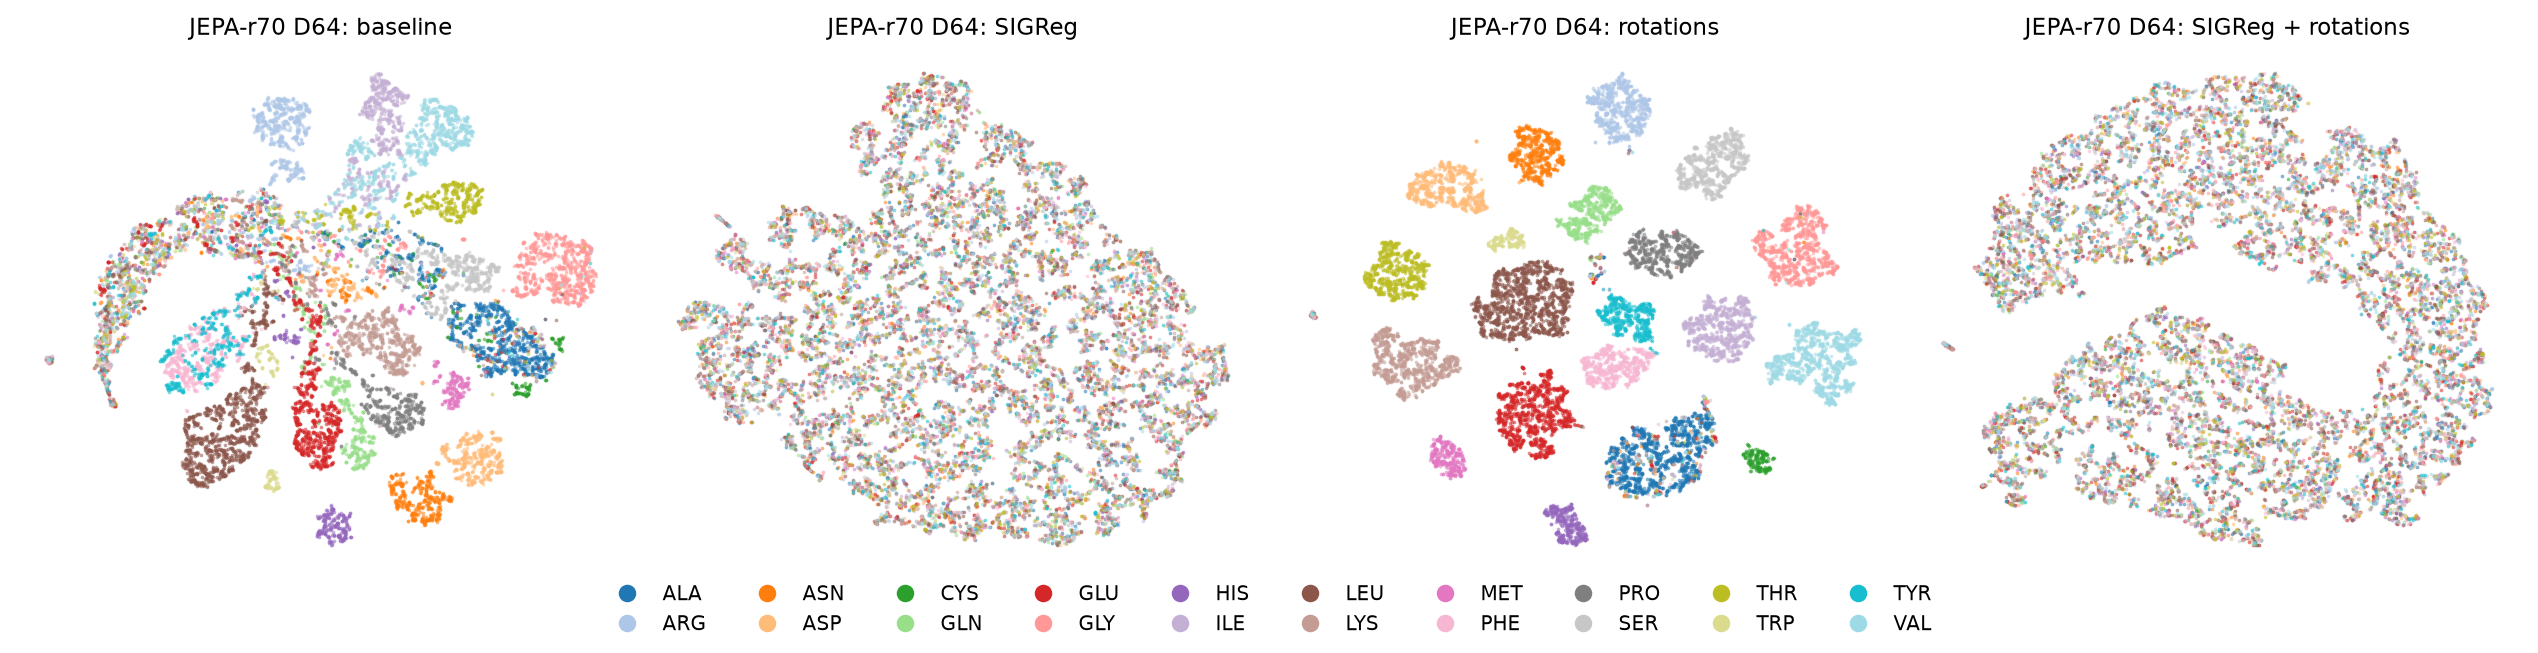
\includegraphics[width=\linewidth]{figures/results/tsne_decisions_exact.png}
\caption{Matched 10k 64D EMA-JEPA design grid: baseline, SIGReg, independent rotations, and SIGReg plus rotations. Points are coloured by amino-acid identity.}
\label{fig:decision-grid}
\end{figure}

We first show the full 100k latent-space roster used throughout the thesis. Figure~\ref{fig:full-latent-grid} compares the same evaluation-residue sample across all models. The reconstruction baselines form amino-acid-separated clusters, standard EMA-JEPA variants are more mixed, the absolute-position JEPA+SIGReg model forms repeated strands, and relative-position variants remove that structure. Random initialisation is included as an architectural control.

We then isolate two design choices in a matched 64D EMA-JEPA screen. Figure~\ref{fig:decision-grid} compares a baseline run, SIGReg, independent $\mathrm{SO}(3)$ view rotations, and SIGReg plus rotations. Rotation produces clear amino-acid clusters in this short-run comparison, whereas adding SIGReg without rotation produces a mixed representation. These visualisations motivate, but do not replace, quantitative invariance and transfer tests.

\clearpage
\section{Supporting Layerwise Evaluation}
\label{app:layerwise-supporting}
\label{app:jepa-r70-layerwise}
\begingroup
\setlength{\intextsep}{4pt}
The matched JEPA random-70 evaluation is complete at all three hidden blocks for BindInt, BindBio, BindShake, CatInt and CatBio.
Across these nine task/split scores, block 6 exceeds the final 8D latent in both model families. It is the strongest of the four readouts on 7/9 canonical LeJEPA scores and 5/9 JEPA scores (Tables~\ref{tab:results-layer-stb} and~\ref{tab:results-layer-stb-jepa-r70}).
This recurrence indicates that the middle-layer advantage is not unique to the canonical LeJEPA objective, although the JEPA results currently cover only this five-task subset.

\begin{table}[H]
\centering
\setlength{\tabcolsep}{4pt}
\renewcommand{\arraystretch}{0.86}
\captionsetup{font=small,skip=3pt}
\fontsize{9}{10.5}\selectfont
\caption{Completed layerwise STB for JEPA with 70\% random masking, using raw/online weights at 100k and full-context evaluation. Hidden-block outputs are 768D and the final latent mean is 8D. Scores are multiplied by 100. Bold marks the strongest readout for each task/split.}
\label{tab:results-layer-stb-jepa-r70}
\begin{tabular}{@{}llrrrr@{}}
\toprule
\multirow{2}{*}{Task} & \multirow{2}{*}{Split}
& \multicolumn{4}{c}{JEPA, random 70\%} \\[1.8pt]
& & Block 1 & Block 6 & Block 12 & Final 8D \\
\midrule
\multirow{2}{*}{BindInt}
& Fold & 47.86 & \textbf{48.86} & 48.24 & 47.11 \\
& SF   & 88.24 & \textbf{91.95} & 91.59 & 80.06 \\
\multirow{2}{*}{BindBio}
& Fold & 72.61 & \textbf{73.22} & 72.84 & 65.56 \\
& SF   & 72.93 & \textbf{73.85} & 73.76 & 65.31 \\
BindShake
& Test & 78.23 & 78.13 & \textbf{78.38} & 71.85 \\
\multirow{2}{*}{CatInt}
& Fold & 65.69 & \textbf{65.72} & 65.05 & 56.84 \\
& SF   & 88.00 & 91.79 & \textbf{92.00} & 76.71 \\
\multirow{2}{*}{CatBio}
& Fold & \textbf{80.72} & 80.13 & 78.23 & 71.50 \\
& SF   & 89.81 & 89.62 & \textbf{90.39} & 75.36 \\
\bottomrule
\end{tabular}
\end{table}

\begin{figure}[H]
\centering
\captionsetup{font=small,skip=3pt}
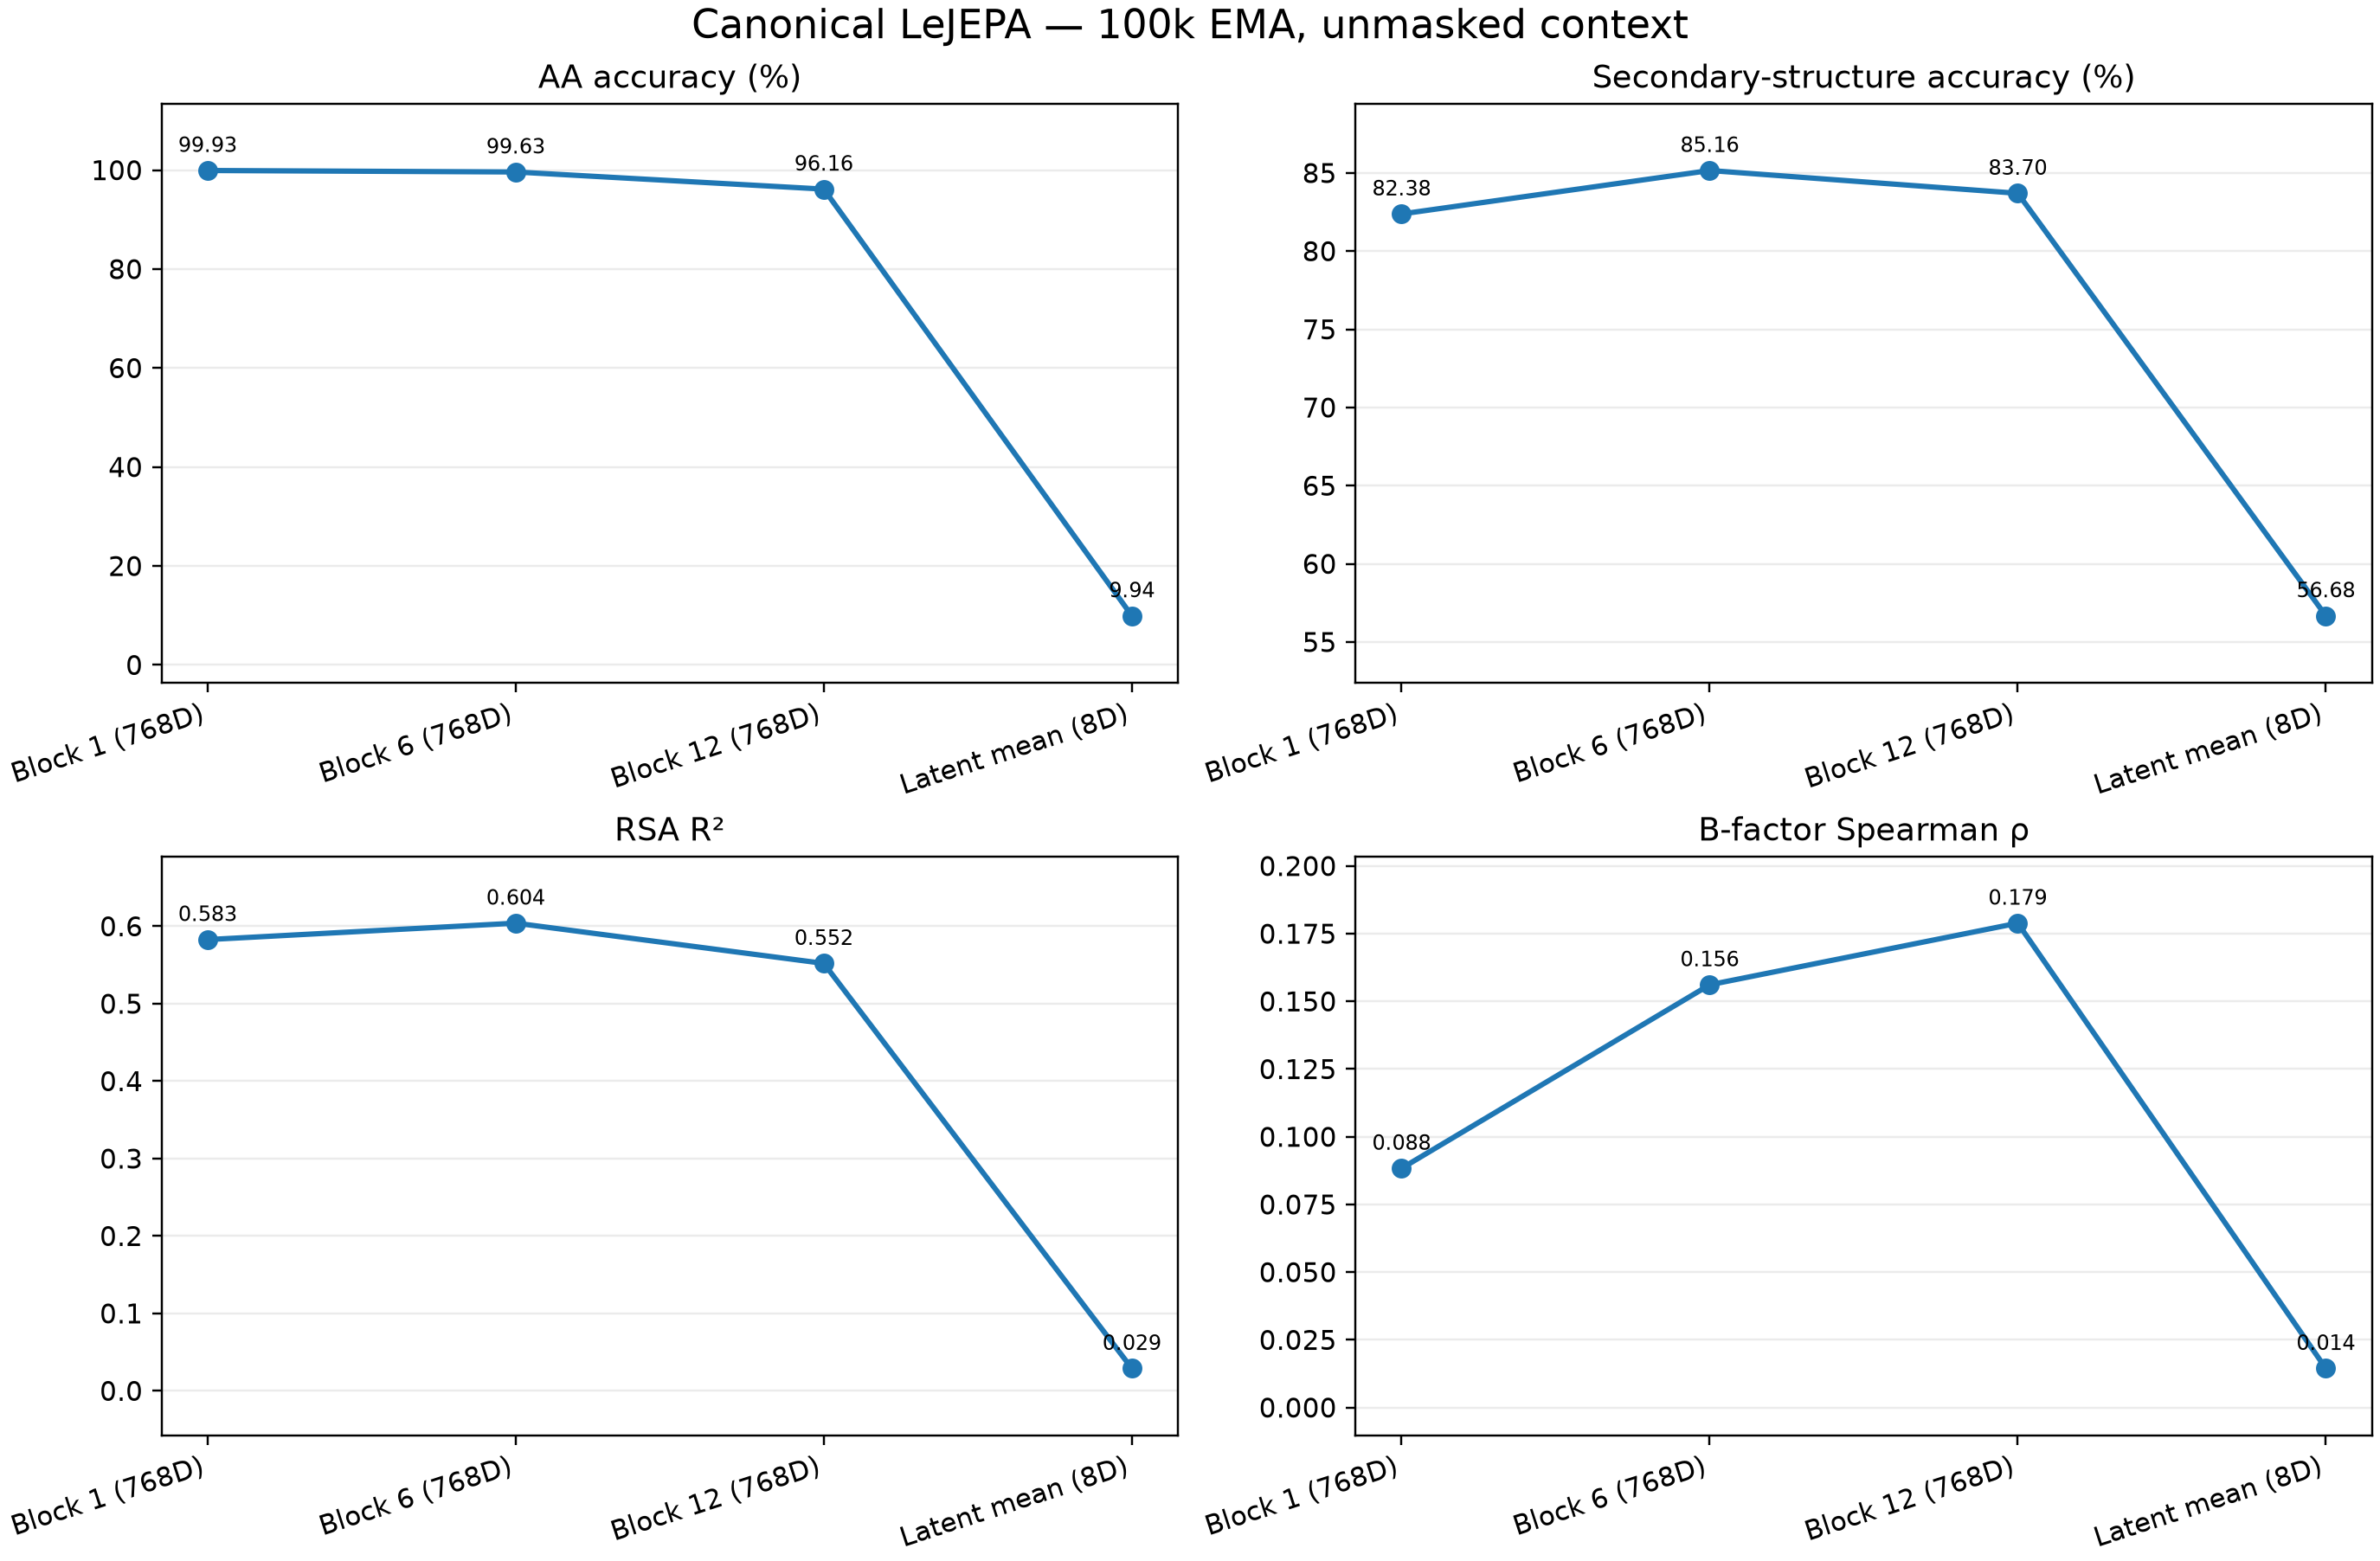
\includegraphics[width=0.80\linewidth]{figures/results/canonical_lejepa_full_context_layerwise_probes.png}
\caption{Full-context linear probes from one uncropped LeJEPA 100k EMA checkpoint. Hidden states are 768D and the final latent mean is 8D. Block-1 SS and block-12 amino-acid/SS fits reported convergence warnings. The highlighted block-6 and latent-mean SS/RSA fits did not. Lines connect different readouts, not a training trajectory.}
\label{fig:results-layer-probes}
\end{figure}
\endgroup
\clearpage

\section{Effect of Encoder Depth}
\label{app:encoder-depth}
Table~\ref{tab:results-encoder-depth} compares the final 8D latent means of separately trained six- and twelve-block uncropped LeJEPA encoders.
Both use seed 42, and the STB cohorts and downstream predictor configurations match.
Each depth was trained once, so the differences have not been checked across independent training seeds.
Training time, memory use and checkpoint sizes are not compared here.

\begin{table}[htbp]
\centering
\setlength{\tabcolsep}{6pt}
\renewcommand{\arraystretch}{0.97}
\captionsetup{font=small,skip=5pt}
\fontsize{8.8}{10}\selectfont
\caption{Full-L600 STB for uncropped LeJEPA with 12 and 6 encoder blocks, without rotations, using raw final-8D latent means at 100k. Scores are multiplied by 100. Bold marks the higher score in each row. $\Delta$ is six-block minus twelve-block. Differences and their unweighted mean across the 24 task/split scores are computed before rounding. This mixed-metric mean is descriptive, not a unified benchmark score.}
\label{tab:results-encoder-depth}
\begin{tabular}{@{}llrrr@{}}
\toprule
Task & Split & \shortstack{12-block\\Final 8D} & \shortstack{6-block\\Final 8D} & $\Delta$ \\
\midrule
\multicolumn{5}{c}{\textbf{Functional-site prediction: AUROC $\times100$}} \\
\midrule
BindInt & Fold & \textbf{50.30} & 45.81 & $-4.49$ \\
 & SF & 88.45 & \textbf{88.58} & $+0.12$ \\
BindBio & Fold & \textbf{59.32} & 59.28 & $-0.04$ \\
 & SF & \textbf{61.82} & 61.41 & $-0.40$ \\
BindShake & Test & 58.45 & \textbf{59.15} & $+0.70$ \\
CatInt & Fold & 51.71 & \textbf{57.13} & $+5.42$ \\
 & SF & \textbf{80.74} & 79.20 & $-1.54$ \\
CatBio & Fold & 53.67 & \textbf{54.06} & $+0.39$ \\
 & SF & \textbf{60.61} & 60.50 & $-0.11$ \\
Con & Fold & \textbf{60.10} & 58.07 & $-2.03$ \\
 & SF & 77.27 & \textbf{78.01} & $+0.73$ \\
Rep & Fold & 71.05 & \textbf{73.05} & $+2.00$ \\
 & SF & 83.49 & \textbf{83.64} & $+0.15$ \\
Ept & Fold & \textbf{62.00} & 54.51 & $-7.49$ \\
 & SF & \textbf{59.72} & 58.83 & $-0.89$ \\
\midrule
\multicolumn{5}{c}{\textbf{Remote homology: macro-F1 $\times100$}} \\
\midrule
Homo & Fold & 6.73 & \textbf{7.73} & $+1.00$ \\
 & Family & \textbf{19.64} & 16.70 & $-2.94$ \\
 & SF & 5.54 & \textbf{6.56} & $+1.02$ \\
\midrule
\multicolumn{5}{c}{\textbf{Structural flexibility: Spearman's $\rho\times100$}} \\
\midrule
FlexRMSF & Fold & 22.48 & \textbf{29.84} & $+7.36$ \\
 & SF & 30.96 & \textbf{41.25} & $+10.28$ \\
FlexBFactor & Fold & 5.01 & \textbf{6.54} & $+1.54$ \\
 & SF & 3.50 & \textbf{5.11} & $+1.61$ \\
FlexNEQ & Fold & 2.46 & \textbf{4.19} & $+1.73$ \\
 & SF & 3.54 & \textbf{5.21} & $+1.67$ \\
\midrule
\multicolumn{4}{l}{Mean difference (6-block $-$ 12-block)} & $+0.66$ \\
\bottomrule
\end{tabular}
\end{table}
\clearpage


\end{document}
